\listfiles
\documentclass[12pt,spanish,letterpaper,oneside]{book}
\usepackage[utf8]{inputenc}
\usepackage[spanish,activeacute,es-lcroman]{babel}	%para incluir los caracteres españoles en el código fuente.
\usepackage{graphicx}
\usepackage{float}		%para que las tablas queden en donde el lugar donde está puesto el código fuente
\usepackage{listings}
\usepackage{color}
\usepackage{url}
\usepackage[breaklinks]{hyperref}
\usepackage{breakurl}	%Con esto por fin se rompieron las líneas del url
\usepackage{listings}	%Para código fuente
\usepackage{fancyvrb}
\usepackage{anysize}	%para establecer los márgenes
\usepackage{fancyhdr}	%Para modificar la posición del número de página
\usepackage{times}
\usepackage[hypcap]{caption} % para que los vinculos lleven al tope de la figura.
% \renewcommand{\baselinestretch}{1.5} % para saltar 1.5 el espacio

\urlstyle{same} % same: mismo formato que el texto | rm,sf,tt,same |

% configuración del código con lslistings
\definecolor{light-gray}{gray}{0.4}
\lstset{numberstyle=\tiny ,basicstyle = \ttfamily ,numbers=left, stepnumber=1, frame=shadowbox,tabsize=4,rulesepcolor=\color{light-gray}}

% Proposition para enumerar y tener referencia a los puntos con un label http://tex.stackexchange.com/questions/11896/labels-for-itemize-in-proposition
\newcounter{prop}[chapter]
\renewcommand*{\theprop}{\thechapter.\arabic{prop}}

\newenvironment{prop}{%
  \refstepcounter{prop}%
%  \paragraph{Proposition~\theprop}%
%  \renewcommand*{\theenumi}{\theprop\,(\roman{enumi})}% esta no para que solo salga el numero romano
  \renewcommand*{\theenumi}{(\roman{enumi})}%
  \renewcommand*{\labelenumi}{(\roman{enumi})}%
  \enumerate
}{%
  \endenumerate
}

%Título
\title{Dise\~no e implementación de aplicaci\'on cliente en dispositivos iOS para la reproducci\'on de medios en un servidor de streaming timeshift.}
          
%Información del autor
\author{
	Javier Cristóbal González Ovalle									\\
	Ingeniería Civil Electrónica								\\
	Universidad Técnica Federico Santa María		\\	
	email:\url{javier.gonzalezo@alumnos.utfsm.cl}	\\
																		\\
	Profesor Guía: Agustín González Valenzuela	\\
	Profesor Co-referente: Tomás Arredondo Vidal		\\
} 
%Márgenes
\marginsize{4cm}{3cm}{3cm}{3cm}
%Fecha	
\date{Agosto de 2012}
\sloppy


%Colocar el número de página abajo a la derecha

%Configuración de las páginas planas.(Con esto logré la posición del número
%en la tabla de contenidos, primera página de capítulo, etc.
 \pagestyle{fancyplain}
 \fancyhf{}
 \rfoot{\thepage}
 
 %\pagenumbering{roman} 
%Estructura del documento
\begin{document}
	%\frontmatter
	%Incluir Portada
	\begin{titlepage}

%Cabecera de presentación de la universidad.
\begin{center}

	\large  UNIVERSIDAD TÉCNICA FEDERICO SANTA MARÍA 	\\
 	\large \sc DEPARTAMENTO DE ELECTRÓNICA						\\
 	\large \sc VALPARAÍSO-CHILE												\\
\vspace*{0.5cm}
\begin{figure}[h!]
	\centering
 	
\includegraphics[scale=1]{imgs/logo_utfsm.eps} 
\end{figure}
\end{center}

%Título de la memoria
\begin{center}
 \LARGE{Diseño e Implementación de Aplicación Cliente en Dispositivos iOS para la Reproducción de Medios en un Servidor de Streaming Timeshift}
\end{center}

%Información del alumnos
\vspace*{1.0cm}
\begin{center}
 \normalsize JAVIER CRISTÓBAL GONZÁLEZ OVALLE\\
 \normalsize MEMORIA DE TITULACIÓN PARA OPTAR AL TÍTULO DE \\
 \normalsize INGENIERO CIVIL ELECTRÓNICO MENCIÓN COMPUTADORES
% \normalsize MENCIÓN COMPUTADORES
\end{center}
\vspace*{1.5cm}

\begin{center}
\begin{tabular}{ll}
 \normalsize Profesor Guía: & Agustín González Valenzuela\\
 \normalsize Profesores Co-Referentes: &Tomás Arredondo Vidal\\
 															&Alfredo Luco Díaz
\end{tabular}
\end{center}
 
\vspace*{2cm}
\begin{center}
 \normalsize Valparaíso, Agosto de 2013. \\
 %\normalsize Material de referencia, su uso no involucra responsabilidad del autor o de la Institución.
\end{center}
\end{titlepage}
	%\begin{titlepage}

%Cabecera de presentación de la universidad.
\begin{center}

	\large  UNIVERSIDAD TÉCNICA FEDERICO SANTA MARÍA 	\\
 	\large \sc DEPARTAMENTO DE ELECTRÓNICA						\\
 	\large \sc VALPARAÍSO-CHILE												\\
\vspace*{0.5cm}
\begin{figure}[h!]
	\centering
 	
\includegraphics[scale=1]{imgs/logo_utfsm.eps} 
\end{figure}
\end{center}

%Título de la memoria
\begin{center}
 \LARGE{Diseño e Implementación de Aplicación Cliente en Dispositivos iOS para la Reproducción de Medios en un Servidor de Streaming Timeshift}
\end{center}

%Información del alumnos
\vspace*{1.0cm}
\begin{center}
 \normalsize JAVIER CRISTÓBAL GONZÁLEZ OVALLE\\
 \normalsize MEMORIA DE TITULACIÓN PARA OPTAR AL TÍTULO DE \\
 \normalsize INGENIERO CIVIL ELECTRÓNICO MENCIÓN COMPUTADORES
% \normalsize MENCIÓN COMPUTADORES
\end{center}
\vspace*{1.5cm}

\begin{center}
\begin{tabular}{ll}
 \normalsize Profesor Guía: & Agustín González Valenzuela\\
 \normalsize Profesores Co-Referentes: &Tomás Arredondo Vidal\\
 															&Alfredo Luco Díaz
\end{tabular}
\end{center}
 
\vspace*{2cm}
\begin{center}
 \normalsize Valparaíso, Agosto de 2013. \\
 %\normalsize Material de referencia, su uso no involucra responsabilidad del autor o de la Institución.
\end{center}
\end{titlepage} si le pongo include no me aparece con la compilación rápida
	
	%Comenzar numeración romana
	\renewcommand{\thepage}{\roman{page}}
 	\setcounter{page}{1}
	
	%Índice General
	\tableofcontents
	\addcontentsline{toc}{chapter}{Índice General}

	%Índice de Figuras 
 	\listoffigures
 	\addcontentsline{toc}{chapter}{Índice de Figuras}

	%Índice de Tablas
 	\listoftables
 	\addcontentsline{toc}{chapter}{Índice de Tablas} 
 
   \newpage
\thispagestyle{empty}
\begin{center}
 \Large \textbf{Diseño e implementación de aplicación cliente en dispositivos iOS para la reproducción de medios en un servidor de streaming timeshift}\\

\normalsize Memoria para optar al título de Ingeniero Civil Electrónico, mención Computadores \\
\normalsize Javier González Ovalle \\
\normalsize Profesor Guía: Agustín González Valenzuela \\
\normalsize Junio de 2012

\Large \textbf{Resumen}

\end{center}
\normalsize
%\textbf{Objetivos del Trabajo:} \\
%\subsection*{Objetivos del Trabajo}
%\normalsize
%Siguiendo el esquema de AHidalgo.pdf

%Siguiendo el esquema de AHidalgo.pdf

%Primer parrafo, descripción breve de los objetivos
El objetivo de este trabajo busca extender hacia los dispositivos móviles el servicio de \textit{streaming} por Internet desarrollado por la empresa AltaVoz S.A. La característica principal de este desarrollo permite al auditor cambiar el tiempo de la reproducción para ver programas pasados, repetir escenas de interés, o permitir pausar el contenido para ser visto más tarde, esta característica lleva el nombre comercial de \textit{timeshift}.\\

%El objetivo de este trabajo es implementar un protocolo de ruteo multi-hop que permita a un sistema de recolección de datos, construido sobre una red de sensores inalámbricos, transportar los datos generados por los sensores a un punto de recolección en la red.\\ 

%Segundo párrafo, contextualizaciòn del problema
El servicio de \textit{stream timeshift} está disponible a través de la plataforma Web exclusivamente para computadores capaces de presentar contenido con Adobe Flash. Cae el problema en el interés de posibles clientes de esta tecnologia, por ejemplo canales de televisión, de llegar a la plataforma móvil, entiéndase teléfonos celulares del tipo smartphone, capaces de reproducir video. Debido a la incapacidad de la gran mayoría de los \textit{smartphones} de cargar el plugin Flash en sus navegadores Web se debe buscar una alternativa para presentar el contenido del \textit{stream} con la caracteristica \textit{timeshift}.
\\

%El sistema de recolección objetivo está orientado principalmente al monitoreo de variables físicas relacionadas con la agricultura como la humedad y la temperatura de los suelos, en zonas de difícil acceso y que no cuentan con redes de distribución eléctrica. La red de sensores inalámbricos que se utiliza para este trabajo está implementada sobre la plataforma de hardware TmoteSky y la plataforma de software TinyOS. En este contexto, se investigan e implementan protocolos que permitan extender el tiempo de autonomía de los nodos al orden de meses.\\
 
%Tercer y cuarto párrafo, que y como se realizó



%Para comenzar, se realiza una investigación de los algoritmos de ruteo para redes de sensores que se han propuesto en la literatura y los protocolos que se han implementado en algunas plataformas. Posteriormente, se realiza una implementación del protocolo PEGASIS y un diseño e implementación de un protocolo de ruteo con topología de árbol que utiliza el componente ''Low Power Listening'' para reducir el consumo energético. Finalmente, se realiza una evaluación energética en la que se determina que con la utilización del componente ''Low Power Listening'' es posible implementar una red con un tiempo de autonomía energética del orden requerido.\\

%Palabras clave.
\textbf{Palabras Claves:} straming, Internet, timeshift, mobile, Apple, iOS, Android, twitter.
%sensores, ruteo, protocolos, algoritmos, energía.

%Primer parrafo, descripción breve de los objetivos
%Nuevos avances se han realizado en el manejo de transmisiones en vivo de medios como audio y/o video, que permiten emular la característica principal de dispositivos de sobremesa del tipo \textquotedblleft Programmable (Digital) Video Recorders\textquotedblright \ (PVR ó DVR), los cuales permite pausar, retroceder o avanzar, cuando es posible, la linea de tiempo de reproducción. Esto se logra gracias a aplicaciones que interactuan con servidores de flujo de datos de audio y video para lograr un registro de la reproducción, entregando al cliente comunicación eficaz para recibir datos y retornar comandos.\\ 
%
%%Segundo párrafo, contextualizaciòn del problema
%Se busca suplir la necesidad de un reproductor de audio y/o video que permita la interacción con un servidor de \textit{streaming} (flujo) de datos, con habilidad de \textit{Time-Shift} (cambio temporal). Esto es la habilidad de retroceder o avanzar (si es posible) en la linea de tiempo de la reproducción del audio o del video al que el usuario atiende.\\
%
%Esto ya se logra en computadores de escritorio gracias a un reproductor de streaming basado en la tecnolog\'ia Flash de Adobe. Los reproductores embebidos en p\'aginas web reproducen el stream en base al protocolo Real Time Messaging Protocol (RTMP), el cual permite llamadas de control entre cliente y servidor para manejar la linea de tiempo. Sin embargo se busca llegar a un mayor público portando la capacidad de reproducci\'on en dispositivos que utilizan el sistema operativo iOS de Apple.\\
%
%El objetivo de este trabajo se debe a que Apple por políticas internas, no apoya la distribuci\'on de Adobe Flash. Por lo tanto se busca implementar una soluci\'on que permita la reproducci\'on de la transmisi\'on con \textit{Time-Shift} y que adem\'as concuerde con las pol\'iticas de distribuci\'on para las aplicaciones iOS en la AppStore.
% 
%\large
%%\textbf{Trabajo a Desarrollar:}\\
%\subsection*{Trabajo a Desarrollar}
%\normalsize
%%Tercer y cuarto párrafo, que y como se realizó
%El trabajo toma como punto de partida la investigaci\'on de los protocolos propuestos por Apple para la distribuci\'on de medios (audio y/o video). En base a estos protocolos buscar similitudes con el sistema de streaming para computadores de escritorio. Adem\'as se busca implementar un m\'etodo de marcaci\'on de tiempo en el stream de datos destinado a dispositivos m\'oviles, de forma que el servidor los env\'ie para que el cliente los interprete. Este cliente debe consistir en una aplicación que reciba y env\'ie comandos compatibles con el servidor Wowza para controlar la informaci\'on del medio a reproducir. Finalmente se busca diseñar una interfaz gr\'afica que represente la disponibilidad de tiempo y permita controlar la reproducción.\\
%
%%\textbf{Evaluaciones a Realizar:}
%\subsubsection*{Evaluaciones a Realizar}
%\normalsize
%\begin{itemize}
%\item	Comprobar la transmisión y recepción de datos en HTTP Live Stream u otro protocolo compatible con iOS, a través de un servidor de streaming dedicado y un dispositivo con iOS.
%\item	Comprobar el intercambio de mensajes de control a través de un enlace entre el cliente móvil y el servidor de streaming.
%\item	Pruebas comparativas de la reproducción en dispositivo móviles y computadores de escritorio.
%\end{itemize}
%
%%\textbf{Resultados esperados:}\\
%\subsubsection*{Resultados esperados}
%\normalsize
%Se pretende que la reproducción en dispositivos móviles de las transmisiones en vivo se asemejen a la experiencia de reproducción en computadores de escritorio.\\

%Palabras clave.
%	\textbf{Palabras Claves:} streaming, iOS, video, audio, apple, iPhone.

   \addcontentsline{toc}{chapter}{Resumen}

   % \newpage
\thispagestyle{empty}
\begin{center}
 \Large \textbf{Evaluation, selection and implementation of a routing protocol for a data collection system based on a wireless sensor network}\\

%\normalsize Memoria (buscar traducción de memoria) para optar al título de Ingeniero Civil Electrónico, mención Computadores \\
\normalsize Luis Enrique Espinoza Severino \\
%\normalsize Profesor : Agustín González Valenzuela \\
\normalsize November 2010

\Large \textbf{Abstract}

\end{center}
\normalsize
The goal of this work is to implement a multi-hop routing protocol that allow to a data collection system, built on a wireless sensor network, move the data generated by sensors to a collection point in the network.\\

The target collection system is oriented to monitoring of physical variables related with agriculture, such as soil humidity and temperature, in areas with difficult access and without electricity distribution networks. The wireless sensor network used in this work is implemented on the TmoteSky hardware and TinyOS software. In this context, energy-aware protocols were investigated and implemented.\\

To begin, in this work is conducted an investigation in routing algorithms proposed in the literature and protocols that have been implemented. Subsequently, is performed an implementation of the PEGASIS protocol. Furthermore, is performed a design and implementation of a routing protocol with a tree topology using the Low Power Listening component to reduce energy consumption. Finally, is conducted an energy consumption evaluation in which is determined that use of the Low Power Listening component enable to deploy a network with the lifetime of the order required.


 
   % \addcontentsline{toc}{chapter}{Abstract} 
 
 	\mainmatter
	%Reiniciar numeración y cambiar a números áraes
	\renewcommand{\thepage}{\arabic{page}} 
	\setcounter{page}{1}
	
	%Configuración del estilo de las páginas generales.(Como el cuerpo)
	\pagestyle{fancy}
	%Colocar el número de página abajo a la derecha
    \fancyhf{}
    \rfoot{\thepage}
    \lhead{\leftmark} 	
	\thispagestyle{fancy}
 	
	%Incluir capítulo 1
	% capitulo1.tex
\chapter{Introducción}

La manera en que se entregan contenidos audiovisuales a los auditores en la actualidad son el resultado de más de un siglo de evolución en materia tecnológica, tanto para el registro de la información, imagen y/o audio, como para las vías de comunicación. Esta evolución está compuesta de hitos científicos que datan del siglo XIX, y entregan una historia rica en avances e investigación destinada al desarrollo de sistemas que entregan información de la mejor forma posible.\\

A lo largo de los años estos desarrollos han significado un cambio en el comportamiento de los auditores, que a su vez han generado o destruido industrias relacionadas a los contenidos audiovisuales. Considerando que el fin de este proyecto de memoria busca implementar una nueva forma de entregar contenido utilizando parte de la tecnología actual, es necesario revisar los sucesos desde el génesis de los registros y comunicación de medios audiovisuales.


%La relación entre el registro de datos audiovisuales y las comunicaciones se han relacionado desde inicios del siglo XIX, es decir 

%El fin de este proyecto es lograr la entrega de contenidos audiovisuales a una nueva audiencia que ha surgido con los últimos avances tecnológicos del siglo XXI, específicamente Internet y la telefonía móvil. 
%La entrega de información a gran escala se encuentra constantemente asociada a los avances tecnólogicos para el registro de imagenes y audio.
%A través de los años el registro de datos de imagen y audio, se ha asociado a la entrega del contenido a una gran cantidad de personas, o auditores. Por lo tanto se deba abordar el inicio de estos registros a el estado actual de las transmisiones.

%Previo al desarrollo del proyecto se debe tener presente la historia y avances tecnológicos relacionados con las transmisiones de medios.

%La historia de los medios es importante por cuanto comprende los avances logrados por el hombre que nos permitieron arribar a los resultados tecnológicos actuales. Lo anterior toda vez que así como la historia de todas las instituciones sociales políticas y económicas del hombre han evolucionado a través de la historia, es la tecnología donde las escalas de avance se han dado en forma más notoria sobre todo en el pasado siglo XX, desde donde por ejemplo de la comunicación por carta manuscrita se logró la comunicación cablegráfica, a mayor abundamiento en materia eléctrica, se logró en menos de 70 años de elevar en vuelo a 2 hombre 1,5 km a poner al hombre en la luna.
\section{Historia de los medios}
%Introducción nueva
%¿Qué son las redes de sensores inalámbricos?
Tomando en cuenta que desde sus inicios la reproducción de medios siempre ha estado relacionada con los últimos avances científicos, los medios de distribución actuales tienen sus orígenes en avances que datan  del siglo XIX.\\

Inicialmente los registros de audio con posibilidades de distribución aparecieron con el invento basado en el fonógrafo de Thomas Alva Edison, como también en el Gramófono de Emile Berliner, aparecido en 1887 y patentado en 1888. La diferencia con el diseño original de Edison está en el medio de registro de audio con el disco de vinilo. Cabe recordar la famosa imagen de la compañía RCA Víctor del Perro escuchando la voz del amo.\\

Análogamente el registro de imágenes en movimiento apareció gracias al cinematógrafo, invento del francés Léon Bouly, y más tarde desarrollado y popularizado por los hermanos Auguste y Louis Lumière, el cual permitió la grabación y reproducción del contenido con la misma máquina.\\

Esta tecnología sienta bases para la transmisión de contenidos a gran escala, \textit{broadcasting}. Para el siglo XX, los avances en tecnología permiten experimentar con difusión a través del espectro de frecuencias.\\

 Ya en el año 1920 la radio es el medio más popular de difusión, llegando a estar presente en 40 millones de hogares estadounidenses, para tres décadas después, en los 1950’s ser reemplazada en popularidad por la transmisión de imágenes y sonidos a través de la naciente televisión.\\

	Estos medios comunicativos para la década actual mantienen su esencia, que es la transmisión del video y/o audio a un gran universo de personas. Si bien el medio por el que se transmite, la resolución, fidelidad, formato y tamaño de los equipos han cambiado, las bases que las fundamentan siguen siendo la transmisión de contenido audiovisual a una gran cantidad de personas, ya sea con fines informativos, de educación o entretención.\\
	
En la actualidad las transmisiones de audio y video se encuentran en un estado de transición desde medios de comunicación análogo como, por ejemplo, la radio FM, AM y la televisión PAL, NTSC, SECAM, a transmisiones digitales. El motivo de este cambio tecnológico es aprovechar de mejor manera el espectro radioeléctrico, enviando la misma o mayor información que por transmisiones análogas, pero utilizando menos recursos del espectro (Subtel Chile \cite{sota:subtel}).\\

Otro medio de transmisión y comunicación global que ha tomado gran significancia en la última década es la Internet. A través de transmisiones de flujos de datos (\textit{streaming}), es posible escuchar radios online, ver videos en YouTube, o utilizar servicios de películas “on-demand” como Netflix, por dar ejemplos disponibles en Chile. Todo esto siendo recibido en un computador u otro dispositivo que presente conectividad a la red.\\

Estos dispositivos alternativos tienen el peso de llevar la recepción de medios audiovisuales por un nuevo rumbo y ya están siendo considerados por las empresas que generan el contenido, al proveer salidas directas a televisores con Internet; consolas de videojuegos con navegador web o aplicaciones cliente para servicios de audio o video on-demand. Otro punto a tener en cuenta es la mayor importancia que tiene el crecimiento del consumo de dispositivos móviles como celulares o reproductores portátiles multimedia, donde se puede llegar a una audiencia aun mayor.\\

Considerando el gran papel que está tomando Internet en el consumo de contenidos, es necesario enfocar el desarrollo de las transmisiones a resultados que aprovechen este medio y llegar asi a la creciente audiencia que lo utiliza. 
Lo cual aportaría en el futuro a igualar o incluso superar en importancia a las transmisiones por internet con las del medio terrestre, tanto digitales como análogas.

\clearpage
\section{Tecnología actual relacionada}
En la siguiente sección se presentan las tecnologías actualmente en uso para la transmisión de medios.

\subsection{Estado actual de las transmisiones}

Considerando que el objetivo de este trabajo tiene relación con la distribución y recepción de contenidos audiovisuales se presentan distintos medios funcionando actualmente.\\

\subsubsection{Video-on-demand}
Es un servicio de distribución que permite a los usuarios seleccionar y ver o escuchar contenidos de video o audio de manera personalizada, ofreciendo la opción de solicitar el material en el momento exacto que lo desee.  La plataforma para poder reproducir el contenido se puede encontrar implementada como aplicación en un computador o a través de un dispositivo con conexión directa al televisor y al proveedor del servicio. En Chile este servicio es provisto por la compañía VTR a través de su dispositivo D-Box, este dispositivo cumple además la función de DVR.\\

La compañía Netflix también provee este servicio, sin embargo el medio de transmisión es Internet, ofreciendo a sus clientes suscripciones que permiten el acceso al catálogo de películas y documentales.\\

En Chile el servicio de \textit{Video-on-demand} entregado por Netflix se ha posicionado a partir de Septiembre de 2011 buscando simplificar el registro de nuevos usuarios, su potencial captación de nuevos usuarios se magnifica al poner a disposición de sus clientes el acceso a los contenidos a través de variadas plataformas de reproducción, como consolas de videojuegos de sobremesa: Nintendo Wii y PlayStation 3, consolas portátiles como Nintendo 3DS, acceso vía web y aplicaciones para televisores con InternetTV. \\

\subsubsection{Podcast}
Es una serie de archivos de medios digitales (audio o video) lanzados en forma periódica por episodios, este sistema permite al usuario descargar el material de su interés para poder reproducirlo más tarde.\\

El modo de distribución se diferencia de otras formas de transferencia de internet como lo son la descarga directa al estar todos los archivos catalogados en un servidor central, éste además provee a los usuarios una vía de distribución a través de RSS Feeds, que son archivos de información en XML (\textit{extended markup language}) diseñados para compartir actualizaciones de sitios web, popularizados por los blogs.\\ 
El uso de RSS Feed para los podcast permite informar a los suscriptores de nuevos contenidos, aunque no es necesario que la persona esté suscrita para obtener alguna información en especifico. 
Su uso se ha popularizado por la plataforma iTunes desarrollada por Apple, que en su versión 4.9 de 2005, abrió a una gran base de usuarios este nuevo medio de comunicación. No solo se utiliza para entregar programas de radio, sino que también documentos y programas de televisión, de manera gratuita.\\

\subsubsection{Streaming media}
Este método provee constantemente datos multimedia al usuario final, que puede reproducir mientras el servidor se encuentra entregando la información.
El nombre se refiere a que el método de entrega es continuo, sin interrupción, debido a que los datos recibidos se almacenan en un buffer de memoria que se va liberando mientas se reproduce. Es decir los datos de audio o video, no son descargados,  es un acceso directo al contenido intangible.\\

Un uso más reciente que se le ha dado al método streaming es lo que se llama \textbf{\textit{LiveStreaming}}, donde el contenido a distribuir es capturado en el momento, una transmisión en vivo que es posible de ser recibida por el usuario casi al momento que ocurre gracias al flujo o stream de datos.\\

La base fundamental de este método de distribución, es la utilización de protocolos ligeros de la capa de transporte, como lo es UDP (\textit{User Datagram Protocol}) que a diferencia del protocolo TCP (\textit{Transmission Control Protocol}), no asegura la entrega en caso de fallo, permitiendo obviar los paquetes, priorizando la continuidad del flujo en el tiempo sobre la fiabilidad de los contenidos.  En la capa de aplicación se ha desarrollado un protocolo con este objetivo, toma como base la conexión mediante UDP para realizar el enlace, es llamado RTP (\textit{Real-time Transport Protocol} \cite{sota:rtp-draft}).\\

Aun así existe un protocolo de la capa de aplicación que utiliza TCP para realizar el enlace. Este fue desarrollado originalmente por Macromedia, siendo ahora propietario \textbf{Adobe Systems}. \textit{Real Time Messaging Protocol} (RTMP \cite{bib:rtmp-specs}) fue desarrollado para realizar streaming multimedia a través de TCP con baja latencia, esto lo logra gracias al envío de la mayor cantidad de información por enlace. \\
	
	De esta metodología \textbf{Apple Inc.} ha desarrollado un nuevo método llamado \textit{\textbf{HTTP Live Streaming}}, que se diferencia al utilizar pedazos de audio o video  ordenados en una lista de reproducción de extensión \textbf{m3u} (\cite{sota:m3u-specs}) que es actualizada a medida que nuevos contenidos son creados. A diferencia del streaming nombrado anteriormente, este flujo de datos se transmite a través del protocolo HTTP (Hypertext Transfer Protocol \cite{sota:rfc-http}), el cual siendo de una capa superior (de aplicación) posibilita la transferencia de los datos multimedia con un servidor web ordinario, como por ejemplo Apache. Además permitir la transmisión en redes donde firewalls o proxies puedan bloquear el contenido, ya que se enmascara como tráfico de hipertexto.


\subsection{Almacenamiento del Contenido}

Otra tecnología que está relacionada con este tema, tiene que ver con la toma de registro de los medios recibidos. Existen en la actualidad los llamados \textbf{DVR} (\textbf{digital video recorders}), dispositivos interactivos que cumplen con la grabación de la señal de televisión o video, siendo almacenada en formato digital.\\

 Esta información queda guardada en el disco duro o memoria del sistema, para poder ser vista después. A diferencia de una antigua videograbadora, el medio de almacenamiento y el formato es digital, permitiendo tomar registro y así manipularlo mediante software.\\
 
	El concepto es aplicado en hardware para televisión e implementado en decodificadores de televisión pagada. En el caso de proveedores de cable, la transmisión es recibida por el enlace coaxial, donde el dispositivo cumple la función de decodificar la señal digital y almacenarla si posee características de DVR.

\subsection{Registros de Stream}

Se puede implementar este concepto de DVR en software de computadores de escritorio, desarrollando alguna aplicación que permita registrar los segmentos transmitidos por streaming para ser reproducidos en otra ocasión. \\

	Servicios de streaming populares como Justin.TV, UStream o Twittcam permiten transmitir video a través de sus plataformas web, y permiten la revisión del contenido tiempo después que este ha finalizado. En cierta parte este comportamiento se asemeja al DVR, pero no posibilita moverse en el tiempo mientras se transmite.\\

En Chile, se ha desarrollado una aplicación más sofisticada por parte de la empresa AltaVoz S.A. con su producto \textquotedblleft SocialStream, Video TimeShift\textquotedblright \ \cite{sota:altavoz-socialstream}, el cual permite retroceder y revisar el contenido mientras la transmisión se encuentra en curso. Este registro es encargado al servidor quien administra los pedazos de información multimedia, una aplicación cliente entabla conexión para realizar pedidos de la información en el tiempo que desea el usuario.
Esta característica lleva como nombre comercial \textbf{TimeShift}.

\section{Propuesta de Proyecto}
\subsection{El Smartphone}
Primero que todo se debe definir el concepto de Smartphone. Para estos efectos lo enteremos como un teléfono portátil con conectividad a las redes celulares y que presenta características adicionales respecto a los teléfonos móviles comunes.\\

Sus bases se sientan en los siguientes conceptos:
\begin{itemize}
\item Su funcionalidad puede ser extendida a través de aplicaciones adicionales.
\item Debe poseer un teclado QWERTY físico o virtual.
\item Debe permitir estar siempre conectado a la Internet.
\end{itemize}
Considerando estos conceptos se puede encasillar como Smartphone a los teléfonos Blackberry, iPhone y Android.

\subsection{Trasfondo}
La mayoría de los smartphones permiten el acceso a internet a través de la red celular utilizando distintas tecnologías de transmisión de datos (no sólo WiFi), como los son actualmente EDGE y 3G. Estas se encuentran en incesante desarrollo, presentando mejoras en la velocidad de transferencia de datos.\\

La constante mejoría en la velocidad de transmisión en redes celulares ha permitido la reproducción de contenidos multimedia. Un avance similar a lo experimentado en la década de 1990 por los computadores multimedia de escritorio. En primera instancia con aplicaciones de contenido audiovisual (imagen, audio, video, texto) ejecutadas localmente, para luego evolucionar y llegar a recibir y transmitir este contenido a través de la world wide web.\\

Los smartphones actuales ejecutan sistemas operativos avanzados que proveen módulos de conexión  a redes, ya sea celular, WiFi, o Bluetooth, si es que el hardware lo incorpora. Además de navegadores web diseñados especialmente para estos dispositivos, con características como presentar en pantalla reducida o ajustada a la resolución, interfaz táctil, teclado numérico, etc.\\

Considerando estas dos importantes bases, conectividad y sistema operativo capaz, es posible implementar una aplicación que se asemeje a la experiencia en computadores de escritorio.\\

\subsection{La Problemática}
El producto desarrollado por la empresa chilena AltaVoz S.A.: \textbf{SocialStream}, destinado a computadores de escritorio y aparatos de sobremesa consiste en una herramienta que permite registrar en el momento, una transmisión en vivo de audio o video. Posibilita al consumidor del contenido, retroceder a un punto en específico, pausar  y avanzar (limitado por el punto más reciente de la transmisión). 
A diferencia de dispositivos de sobremesa (\textbf{set top boxes}) como lo son TiVo u otros DVR, el registro de la transmisión es encargado al servidor quien provee los contenidos a los clientes que se han conectado, y estos contenidos no son guardados localmente. \\

Este sistema nos significan los siguientes beneficios: 
\begin{itemize}
\item Ahorro para el consumidor, espacio en sus dispositivos de almacenamiento
\item Cierto control del proveedor sobre la distribución  y copia de los contenidos
\item La posibilidad de portar a otras plataformas como consolas de videojuegos o dispositivos móviles.
\end{itemize}

Las bases de esta herramienta se fundan sobre Adobe Flash gracias a su protocolo RTMP. Y considerando las diferencias tecnológicas entre Apple y Adobe (ver \cite{sota:steve-flash} carta de Steve Jobs, ex-CEO de Apple Inc.) surge nuestro principal problema:

\begin{itemize}
\item Las aplicaciones que cumplen la función de reproducción de los contenidos están desarrolladas en el lenguaje de programación ActionScript, propio de Adobe.
\item En las plataformas de escritorio y algunos smartphones, esto no significa un problema. Sin embargo los dispositivos de Apple con el sistema operativo iOS no presentan compatibilidad con estas tecnologías Flash.
\end{itemize}

	En las siguientes figuras \ref{sshot_Android_sstream} y \ref{sshot_iOS_sstream} se puede notar claramente el problema que genera en iOS la falta de soporte de tecnologías Adobe.

%\clearpage 
\begin{figure}[h!]
	\centering
	% \fbox{ } % la encierra en un cuadrado, sirve para código también
	 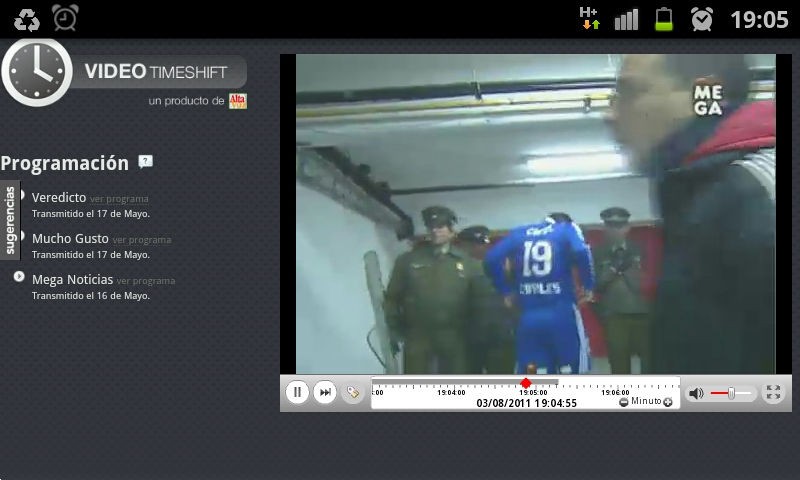
\includegraphics[scale=0.47]{imgs/sshot_Android_sstream.jpg}
 	\caption{Reproducción de SocialStream en Android OS.}
	\label{sshot_Android_sstream}
\end{figure}
%\vspace{3cm}
\begin{figure}[h!]
	\centering
	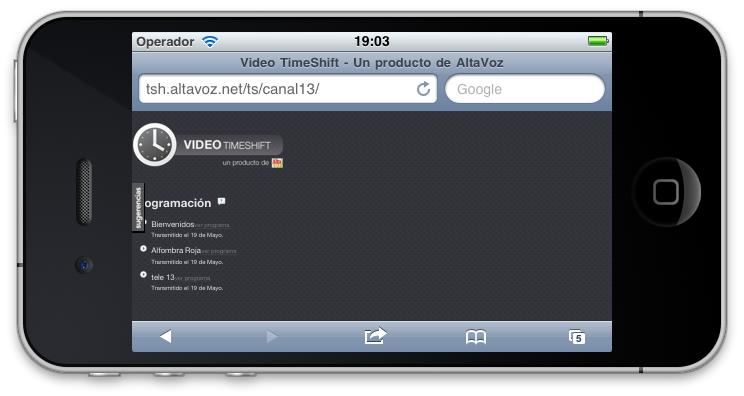
\includegraphics[scale=0.55]{imgs/sshot_iOS_sstream.png}
	\caption{Reproducción de SocialStream en iPhone con iOS}
	\label{sshot_iOS_sstream}
\end{figure}

\newpage
\subsection{Posibles Soluciones}

A la fecha, las herramientas de distribución de audio y/o video por streaming, están limitadas a los reproductores provistos por la interfaz de programación de aplicaciones (API) de iOS. En donde al reproducir contenido por streaming presentan la opción de retroceder la cantidad de  tiempo almacenada en el buffer de datos. \\

%\clearpage
\begin{figure}[h!]
	\centering
	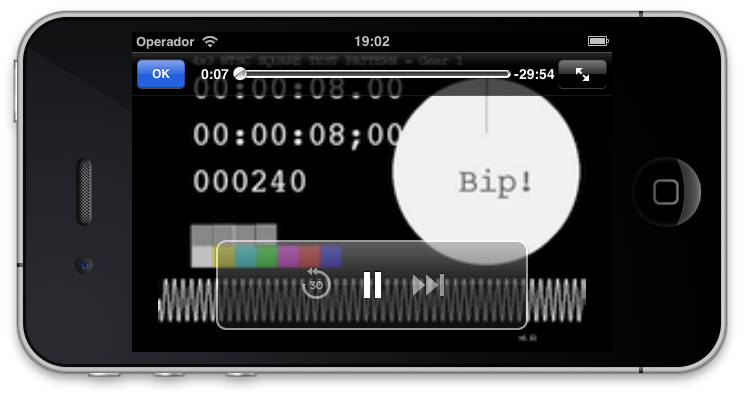
\includegraphics[scale=0.55]{imgs/sshot_iOS_hls.png}
	\caption{Reproducción de flujo video por HTTP Live Streaming}
	\label{sshot_iOS_hls}	
\end{figure}

De la figura \ref{sshot_iOS_hls} se puede notar el botón a la izquierda en la barra inferior de  la pantalla, este hace retroceder en 30 segundos la reproducción.\\

Esta característica es propia del framework MediaPlayer. que simplifica de gran manera la necesidad de mostrar video en el dispositivo. Este uso también se puede aplicar para la reproducción  de  audio y video.
Se debe dejar claro que Apple es sumamente restrictivo en el uso de la API de iOS. \\
Para el desarrollo de aplicaciones, estas deben utilizar solo llamadas al sistema que estén indicadas en sus documentos guía, por lo tanto una vía para desarrollar una solución de reproductor que provea la posibilidad de saltar en la línea del tiempo de reproducción sin importar que tan larga sea la transmisión en vivo, depende de las bases MediaPlayer. \\

En la documentación actual de iOS v4.3 se encuentra AVPlayer (audio video player) [link] que pone a disposición las llamadas y manejo de datos de audio y/o video.


\subsection{Soluciones actuales}
En computadores de escritorio, existen reproductores hechos en Flash que permiten la reproducción de transmisiones de streams en vivo de video FLV y audio en AAC.\\

	En el caso de smartphones, solamente el sistema operativo Android permite mostrar contenido Flash destinado a computadores de escritorio. Por lo tanto la reproducción de videos en formato FLV y audio AAC está asegurada gracias a la carga del reproductor programado para ese propósito.\\

Se encuentra en desarrollo una salida de datos del servidor de medios Wowza, esta salida está basada en la tecnología HTTP Live Streaming, sistema impulsado por Apple para la transmisión de audio y video a través del protocolo de transferencia de hipertexto. Esta característica de Wowza permite reproducir video con  saltos en el tiempo y al no utilizar el encapsulado FLV, es compatible con las tecnologías de iOS.

\subsection{Pros y Contras de una nueva solución}
En el caso de la salida con \textit{HTTP Live Streaming} estándar de Wowza, se puede considerar como punto en contra la interfaz gráfica que no se adecua para el control de la transmisión en caso que esta sea muy amplia. Otro punto en contra es que esta solución significa un costo monetario por pago de licencias de transmisión.\\

	También se puede tomar como punto en contra el hecho que la salida de HTTP Live Streaming es reproducida por el MPMediaPlayer estándar, sin mucha versatilidad para caracteristas expansivas, como por ejemplo integrar redes sociales como twitter o facebook.\\

	En el caso de otros smartphones y sistemas operativos, la reproducción del stream de datos está permitida si es que el sistema operativo soporta Adobe Flash.\\

	Un punto en contra de Android es la variabilidad del hardware que corre dicho sistema operativo. Existiendo distintos modelos y versiones de aparatos compatibles con él, pueden o no presentar los contenidos de forma correcta, por ejemplo dispositivos con procesadores (CPU) de uno o múltiples núcleos, o también la incorporación de procesadores gráficos (GPU) que permiten la decodificación del video por hardware.\\

En el caso de los dispositivos iOS, todos estos son diseñados y construidos por Apple Inc., siguiendo un estándar que permite una experiencia similar en los distintos productos.

\subsection{El beneficio de llegar a nuevas audiencias}
Se debe tomar en cuenta que los dispositivos iOS, entiéndanse iPhone, iPad y iPod Touch; representan una gran participación en cada uno de sus mercados: smartphones, tablet-pc y reproductores  multimedia, respectivamente. Su fuerte y enfoque principal es el mercado de smartphones (fig. \ref{market-share-2012q1}), llegando muy cerca al líder Android de Google 59\% que abarca una gran cantidad de fabricantes de hardware. Si se toma en cuenta que Apple Inc. es el único fabricante del iPhone, su 23\% de participación es de gran importancia.\\

iPad domina el mercado con un 62.8\% de participación (fuente: \cite{sota:iPad-market}), en el área de computadores tipo tablilla (tablet-pc), debido a que este producto introdujo la innovación y la pauta de diseño para sus competidores, que aun no logran igualar la experiencia para el usuario con versiones modificadas de Android, mientras que iOS toma sus bases en el ya consolidado Mac OS X.\\

En el caso de los reproductores multimedia, la popularidad de los dispositivos iPod desde los principios de la década de 2000, ha facilitado la adopción de la línea más reciente que también corre iOS.\\

Tomando en cuenta los puntos indicados anteriormente, se deduce que no son dispositivos que se deben obviar. Al no poseer una aplicación compatible con el sistema de distribución de contenidos, se está acotando una gran parte de la audiencia.\\

En resumen, estos puntos ayudan a presentar que es viable un reproductor alternativo, ya sea como aplicación o biblioteca de desarrollo para nuevos proyectos. \\

\begin{figure}[H]
	\centering
	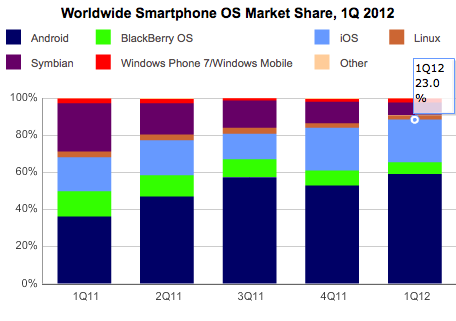
\includegraphics[scale=0.8]{imgs/market-share-2012q1.png} 
	\caption{Participación de iOS en el mercado de sistemas operativos para Smartphones. Fuente \cite{sota:market-smartphones}}
	\label{market-share-2012q1}
\end{figure}



%¿Cuáles son las áreas de investigación y desarrollo de WSN?
%buscar como continuar después de una itemezación con dos puntos y separados por comas.

%Presentar el tema del ruteo y recolección de datos

%IR DE LO GENERAL A LO PARTICULAR!
%El capítulo de introducción debe comenzar explicando que son las 	WSNs.
	%\section{Redes de sensores inalámbricos}
	
	%\section{Aplicaciones}
%En el mundo

%En Chile

	%\section{Protocolo de ruteo para un sistema de recolección de datos}
	%\section{Visión general de los requerimientos}
%Hablar de la aplicación objetivo y cuáles son sus requerimientos 

%Títulos alternativos
% El objetivo de este trabajo es implementar un protocolo de ruteo multihop como parte de un sistema de recolección de datos que está construido sobre una red de sensores inalámbricos. Este sistema está orientado principalmente al monitoreo de variables físicas principalmente relacionadas con la agricultura, como la humedad y la temperatura de los suelos, en zonas de difícil acceso y que no cuentan con redes de distribución eléctrica.

%En el marco de este trabajo, los objetivos generales son los siguientes:
%\begin{enumerate}
%  \item Informar sobre los protocolos de ruteo de mensajes para redes de sensores inalámbricos.
%  \item Desarrollar una red de sensores inalámbricos, utilizando la plataforma de hardware TmoteSky.
%  \item Desarrollar una aplicación para la recolección de datos de la red.
%  \item Evaluar el consumo energético de la red implementada.
%\end{enumerate}

% El primer objetivo se desarrolla en profundidad en el capítulo 2. El segundo objetivo se desarrolla en los capítulos 3, 4 y 5, donde se plantea un diseño de protocolo y posteriormente como se implementa éste. El tercer objetivo se desarrolla en los capítulos 3 y 5 como parte de las verificaciones del sistema. Finalmente, en el capítulo 5 se evalúa el consumo energético el protocolo.\\
 
	%\section{Estado del Arte}


%\subsection{Protocolo de ruteo}
%\begin{figure}[H]
 %\centering
 %\includegraphics[scale=0.8]{imgs/PilaModeloOSI.eps}
 %\caption{Pila de red establecida por el Modelo OSI}
%\end{figure}

	% \subsection{Algoritmos de ruteo propuestos en la literatura}

%En esta sección debería dar una breve reseña  de cada protocolo, con sus referencias.
	%\subsection{Protocolos implementados}

	%\subsection{Hardware de desarrollo}
%De lo general a lo particular
% Qué tipo de hardware existe?

%Debo incluir info sobre los motes que soportan tinyos
	% \subsubsection{Plataformas TinyOS}
	%\subsubsection{Plataformas Zigbee}
	
%Debo incluir info sobre los motes que soportan Zigbee, simpliciti.
	% \subsubsection{Otras plataformas}
	%\subsection{Software para redes de sensores inalámbricos}

%TinyOS, ZStack, SimpliciTI, etc
%Breve descripción de tinyOS e indicación para revisar el anexo XX.
	%\subsubsection{TinyOS}
	%\subsubsection{Contiki}

%Breve descripción de ZStack, basarse en pagina de ti del zstack
	%\subsubsection{Z-Stack}

%Breve descripción de SimpliciTI, basarse en pagina de ti de simpliciti
	% \subsubsection{SimpliciTI}

%Breve descripción de la de los sunspots, basarse en documentacion
	%\subsubsection{Java y SunSpot}

%Breve descripción de alguna otra de otro fabricante..freescale o atmel.


	
	%Incluir capítulo 2
	% capitulo de implementación
\chapter{Diseño e Implementación}
En el siguiente capítulo se describen las etapas recorridas para llegar a la solución que propone este proyecto.
\section{Arquitectura de la solución}
El siguiente capitulo consta de las bases necesarias para realizar la solución, la que se compone de dos elementos principales. 
\begin{itemize}
\item Servidor: Encargado de recodificar (si es necesario) la fuente de audio o video y segmentarla para su distribución.
\item Cliente: Aplicación ejecutada en iOS, encargada de comunicarse al servidor para pedir el flujo de video y entregar información en twitter.
\end{itemize}
% poner figura aqui
La figura \ref{diagramaGral} presenta una idea general del sistema.\\

\begin{figure}[H]
	\centering
	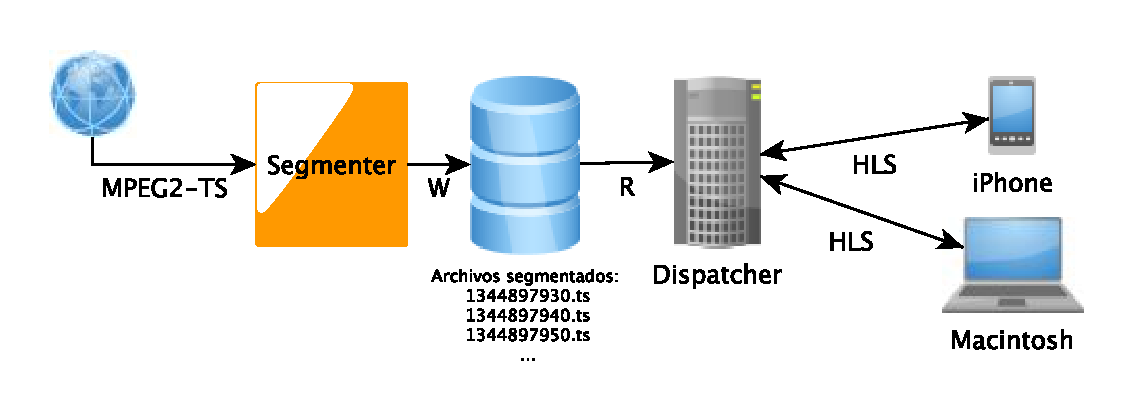
\includegraphics[scale=0.8]{imgs/diagrama_general.eps}
	\caption{Diagrama general de la solución}
	\label{diagramaGral}
\end{figure}

Respecto a los elementos principales, estos se componen de distintos modulos que serán explicados con más detalle a lo largo del capítulo. Del diagrama se explican de forma general:
\begin{itemize}
\item Segmenter: es una aplicacion que recibe como entrada un flujo de audio y/o video encapsulado en MPEG2-Transport Stream, para luego segmentar el contenido en archivos de menor duración, estos se guardan en el sistema de archivos del servidor.
\item Dispatcher: Este es un programa dedicado a recibir peticiones de los clientes, para entregar un flujo de video mediante el protocolo HTTP Live Streaming.
\item iPhone y Macintosh: Son los dispositivos clientes controlados por el usuario, en estos se realiza el intercambio de ordenes para recibir el flujo de video que se quiere ver.
\end{itemize}

\subsection{Requerimiento Obligatorio}
% https://developer.apple.com/news/index.php?id=02162010a
	El protocolo utilizado para entregar el contenido audiovisual es \textit{HTTP Live Streaming} (HLS), el que se eligió debido a requerimientos obligatorios designados por Apple para la distribución de contenidos multimedia para su sistema operativo iOS.\\
	
	En un anuncio realizado por Apple en su sitio web destinado a desarrolladores, indica como obligación que la entrega de contenido del tipo audio y/o video con una una duración mayor a 10 minutos debe utilizar necesariamente el protocolo \textit{HTTP Live Streaming} ya sea el enlace mediante WiFi o red celular. Además las aplicaciones deben incluir un flujo de datos (\textit{stream}) de baja calidad con una cadencia de datos no superior a 64 Kilobits/segundo, de manera que estas aplicaciones mantengan fluidez de contenido a pesar de encontrarse en condiciones desfavorables en la red.
	
	En caso de no seguir esta indicación, el desarrollador arriesga que su aplicación no sea admitida en la plataforma principal para la distribución de aplicaciones: iTunes Store.

	Considerando que este trabajo de memoria busca incorporar a los dispositivos iOS como consumidores del contenido multimedia utilizando saltos temporales (TimeShift), se debió diseñar la solucion alrededor de este protocolo.

%en resumen un acercamiento a como funciona la cosa

%\part{Primera parte}
\section{Protocolo HTTP Live Stream}
% https://developer.apple.com/resources/http-streaming/
% http://en.wikipedia.org/wiki/HTTP_Live_Streaming
% http://en.wikipedia.org/wiki/Progressive_download
% http://en.wikipedia.org/wiki/HyperText_Transfer_Protocol

El protocolo \textit{HTTP Live Streaming} o HLS (abreviado), es un protocolo desarrollado por Apple Inc. para la distribución de multimedia a través de redes de computadores, de manera que el usuario consume el producto a medida que se descarga, es decir de forma continua.\\

Su carácteristica principal es la utilización del protocolo para transferencias de hipertexto, HTTP (\textit{hypertext transfer protocol}) por sus siglas en inglés. Si bien HTTP se diseño originalmente para la \textit{\textbf{World Wide Web}} como vía de entrega del texto en formato HTML, este se puede utilizar para distribuir datos de otros formatos codificados para habilitar su distribución.\\

HLS funciona entregando el contenido de forma segmentada al cliente, el cual tiene la responsabilidad de manejar la lógica de cambio de segmentos. Para distribuir el contenido se codifica la fuente de audio y/o video en varios archivos de corta duración, recomendandose 10 segundos \cite{bib:tensec-targetduration}, y que pueden o no tener el mismo bitrate. Estos pequeños archivos se ordenan en una lista de reproducción de formato .M3U8 que se entrega al reproductor del cliente. \\

También existe una variante donde la lista de reproducción contiene referencias a otras listas de reproducción con otras variantes de flujos de datos. \\

% http://www.streamingmedia.com/Articles/Editorial/What-Is-.../What-is-HLS-(HTTP-Live-Streaming)-78221.aspx
% In the Apple App Store, if you produce an app that delivers video longer then ten minutes or greater than 5MB of data, you must use  HTTP Live Streaming, and provide at least one stream at 64Kbps or lower bandwidth. Any streaming publisher targeting iOS devices via a website or app should know the basics of HLS and how it’s implemented.
	\subsection{Especificación}
		El protocolo HLS consiste en ordenar la entrega de archivos discretos a través de HTTP.
		El procedimiento general consiste en segmentar el contenido multimedia (audio y/o video) en pequeños archivos de manera que a través de un servidor web regular el cliente pueda descargar y unir los segmentos para verlos de manera continua. Esta forma de entregar el contenido puede ser utilizada para contenido pre-grabado o en vivo, difiriendo levemente en el componente encargado de ordenar los segmentos.\\
		
\begin{figure}[H]
	\centering
	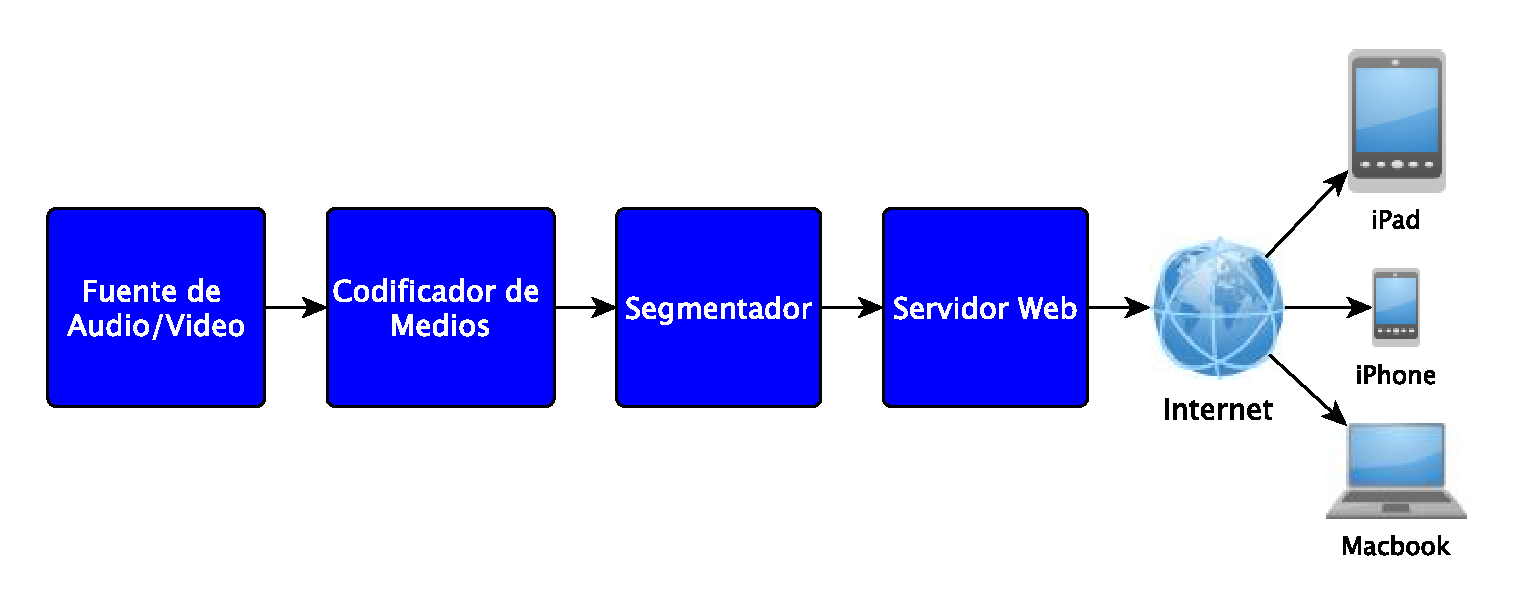
\includegraphics[scale=0.5]{imgs/HLS_diagram_wwdc2010.eps}
	\caption{Flujo de trabajo de HTTP Live Streaming}	
	\label{diagramaHLSwwdc2010}
\end{figure}		
		La figura \ref{diagramaHLSwwdc2010} presenta un ejemplo de distribucion de multimedia a través de HTTP Live Streaming.\\
		
En primera instancia se debe obtener contenido multimedia ya sea en un archivo fijo o flujo de datos, este contenido debe ser codificado para que sea compatible con los dispositivos que corren iOS, generalmente por recomendación de Apple se deben utilizar los codec de video h.264 y de audio AAC (\textit{Advanced Audio Coding}). El empaquetado de este contenido ya codificado debe ser entregado a una aplicación encargada de segmentarlo en pequeños archivos. \\

	El flujo de transporte a utilizar es MPEG2-TS (\textit{MPEG2 Transport Stream}), el resultado de la aplicación segmentadora es guardado en el sistema de archivos donde reside el servidor web (o una ubicación accesible) de manera que al recibir requerimientos de stream HLS, este pueda proveer una lista de reproducción en formato M3U8 que mantiene el orden de reproducción de los archivos.\\
	
Tomando en cuenta el funcionamiento del protocolo HLS, para distribuir el contenido multimedia generado en vivo se debe codificar y segmentar inmediatamente para que el servidor web pueda proveerlos. En el caso de que el contenido sea un gran archivo, la codificación y segmentación se realiza una sola vez.

\subsubsection{Lista de reproducción}
\label{TAG-SECTION}
La lista de reproducción en formato M3U8 es lo que se entrega al cliente, el cual puede ser una aplición iOS o el navegador web Safari desarrollado por Apple. Esta lista consiste en enlaces (URL) absolutos o relativos de los segmentos siguiendo el orden del contenido. Además se incluyen comentarios precedidos por el caracter \textbf{\#}, en el caso que un comentario utilice una palabra conocida del protocolo se le denomina entonces como marca (tag).
Las marcas primordiales para una trasmision a través de HLS son las siguientes:

\begin{prop}

\item \textbf{\#EXTM3U}: Corresponde a la primera marca que inicia una lista de reproducción, siempre debe estar al principio.

\item \textbf{\#EXT-X-TARGETDURATION}: Esta marca corresponde a la mayor duración que puede poseer cualquier segmento, es decir los segmentos enumerados en la lista no pasarán del tiempo especificado por esta marca.
Además este valor indica al cliente cada cuanto tiempo debe realizar una petición al servidor web por la lista.
\label{TAG-targetduration}

\item \label{TAG-mediasequence} \textbf{\#EXT-X-MEDIASEQUENCE}: Corresponde a la secuencia o versión de la lista de reproducción segun los segmentos que se incluyen dentro de ella. Este valor se representa por un número entero y debe ser consecuente a los cambios en el contenido, es decir, si se agregan nuevos segmentos el valor de la secuencia debe aumentar, de esta forma el cliente puede saber que el flujo de contenido se está actualizando.


\item \label{TAG-extinfint} \textbf{\#EXTINF}: Esta marca indica la duración del segmento que se encuentra junto a él. Su valor está indicado por un número entero que representa los segundos.\\
\end{prop}

\begin{figure}[H]
	\centering
	\begin{lstlisting}
	#EXTM3U
	#EXT-X-TARGETDURATION:10
	#EXT-X-MEDIA-SEQUENCE:1
	#EXTINF:10,
	http://media.ejemplo.com/segmento0.ts
	#EXTINF:10,
	http://media.ejemplo.com/segmento1.ts
	#EXTINF:10,
	http://media.ejemplo.com/segmento2.ts
	#EXT-X-ENDLIST
	\end{lstlisting}
	\caption{Lista de reproducción del tipo Video-on-Demand}
	\label{ejemploM3U8}	
\end{figure}			

El ejemplo visto en la figura \ref{ejemploM3U8} destaca una marca extra: \#EXT-X-ENDLIST, la cual indica al cliente que la lista de reproducción está completa y no necesita ser actualizada. Esta marca toma gran importancia al definir un flujo de medios ``en vivo'' ya que al estar ausente el cliente pedirá una nueva versión de la lista de reproducción que incluya nuevos segmentos, el tiempo que indica la actualización depende de la marca \ref{TAG-targetduration} previamente explicada.\\

En el caso de contenido en vivo, la lista de reproducción toma el rol de \textbf{ventana de reproducción}  como la lista se actualiza con nuevos segmentos cada intervalo de \ref{TAG-targetduration} se evita un archivo de gran tamaño al eliminar segmentos ya pasados.

Cabe destacar que la marca \ref{TAG-mediasequence} debe mantener consistencia con los nuevos segmentos, es decir si la lista elimina un segmento pasado y agrega uno nuevo, el numero de secuencia debe aumentar su valor.\\

Para efectos de la solución de este trabajo de memoria el modo de flujo de datos a utilizar con HLS es del tipo ``en vivo''.
\subsubsection{Segmentos}
Los segmentos consisten en video codificado con h.264 y audio en AAC. Apple indica que también es compatible MP3, sin embargo se decidió por AAC debido a su mayor compresión de audio y permitiendo así transmitir un mejor sonido a menor ancho de banda. En el sitio web \cite{apple-hlsencoding} se indican los perfiles recomendados para codificar el contenido a trasmitir con HTTP Live Streaming, para mantener compatibilidad con clientes que estén adoptando el protocolo se utilizó  
\begin{itemize}
\item Video: H.264 Baseline Profile Level 3.0, resolución 480x320 y tasa de fotogramas 29.97

\item Audio: AAC-LC, 48 kHz, stereo.

\end{itemize}

La duración de los segmentos se limitó a 10 segundos por recomendación del mismo documento técnico (TN224 \cite{apple-hlsencoding}), donde indica explícitamente: \textit{\textquotedblleft Use 10 second Target Durations"}, utilice 10 segundos de duración de objetivos.

% El contenedor de los medios es MPEG2-TS según la especificación del protocolo HLS. Las indicaciones de Apple sugieren tener cuidado con el overhead.
		% mostrar figura de playlist, explicacion rapida de como funciona hls
\subsubsection{Borrador IETF}
Apple Inc. es la compañía desarrolladora de este protocolo. Para masificar su uso en dispositivos móviles ha dispuesto un borrador como propuesta para la estandarización del protocolo según la \textbf{IETF} (\textit{Internet Engineering Task Force}).
Debido a la popularidad de los dispositivos móviles con iOS, empresas importantes en el desarrollo de tecnologias para difusión de medios han adoptado el protocolo HLS como salida de productos dedicados a la codificación y/o transmisión de multimedia. Ejemplos como Adobe Systems con su producto Adobe Flash Media Server, Wowza Media Systems con Wowza Media Server y VideoLan con VLC Media Player demuestran que la investigación realizada por los ingenieros de Apple Inc. Roger Pantos y William May, Jr, han sentado las bases para cualquier desarrollo asociado con el protocolo.\\

Para el desarrollo de esta memoria se han implementado aplicaciones y scripts que utilizan las herramientas e instrucciones detalladas en el documento borrador. A lo largo de la investigación los ingenieros desarrolladores incorporaron caracteristicas nuevas que fueron aprovechadas para lograr el cometido de esta memoria.\\

En sitio web \cite{apple-draftpantos} se puede revisar detalladamente el documento completo. En esta sección se describen las marcas utilizadas aparte de las ya descritas en \ref{TAG-SECTION}:

\begin{itemize}
\item \textbf{\#EXT-X-VERSION}: Corresponde a la versión de la lista de reproducción, se utiliza para diferenciar distintos streams con protocolo HLS según las caracteristicas que se van incorporando. Para el trabajo de esta memoria se utiliza la versión 3 del protocolo.

\item \textbf{\#EXTINF}: Si bien ya se ha descrito esta marca en \ref{TAG-extinfint}, a partir de la versión 3 del protocolo HLS ésta permite valores flotantes para mejorar por parte del cliente la exactitud en el seguimiento del tiempo de reproducción. 

\item \textbf{\#EXT-X-PROGRAM-DATE-TIME}: Marca correspondiente a la fecha asociada al primer segmento de datos que aparece en la lista de reproducción. La fecha se especifica utilizando el estandar ISO 8601, y opcionalmente se puede incluir zona horaria. Un ejemplo del formato sería:

\begin{lstlisting}
#EXT-X-PROGRAM-DATE-TIME:2011-12-18T14:54:23-04:00
\end{lstlisting}

Correspondiente al día 18 de diciembre de 2011, a las 14:54:23 en la zona horaria GMT-4.

\end{itemize}
		% aqui detallar los mensajes de la playlist utilizados
		%		http://tools.ietf.org/html/draft-pantos-http-live-streaming-08
\subsubsection{Lista de Variantes}
Más allá de la lista de reproducción con segmentos, el protocolo HLS posee caracteristicas anexas para mejorar la experiencia del usuario.
Una de las caracteristicas a utilizar y que también es requisito para que las aplicaciones con multimedia remota puedan ser aprobada en la App Store es la necesidad de una variante del stream por donde se transmita solamente el audio.\\

Para solucionar este requerimiento y cumpliri la obligación se utiliza una lista de variantes, la cual consiste en una lista de reproducción que incluye en su interior URLs hacia listas de reproducción normales ya explicadas anteriormente, la diferencia cae en que cada lista de reproducción tiene asociado un ancho de banda límite, de manera que el cliente pueda cambiar de stream dentro de la reproducción sin que el usuario note el cambio en la reproducción, exceptuando la calidad del audio o del video.\\

Se utiliza la marca \textbf{\#EXT-X-STREAM-INF} para asociar cada una de las variantes del stream a cierto ancho de banda, además cada una posee los siguientes atributos:

\begin{itemize}

\item \textbf{PROGRAM-ID}: Corresponde a un valor numérico entero, tiene como fin identificar una presentación en particular dentro de la ventana de transmisión de la lista de reproducción. Una lista de variantes puede contener multiples sublistas con distintos programas de forma que este atributo asocia las distintas variantes para una transmisión en particular, entiendase por show o evento a transmitir. Esta caracteristica puede ser opcional.

\item \textbf{BANDWIDTH}: Este atributo obligatorio representa el valor entero de los bits por segundo, como requisito principal el valor debe ser la cota mayor de la tasa de bits promedio de los segmentos (incluyendo el overhead del contenedor) que aparecen o aparecerán en la lista de reproducción. 

\end{itemize}

El enlace a las sublistas de variantes del stream pueden ser del tipo relativo o absoluto. Como requisito cada variante del stream debe poseer el mismo valor en segundos de Target Duration \ref{TAG-targetduration}.

\begin{figure}[H]
	\centering
	\begin{lstlisting}
	#EXTM3U
	#EXT-X-STREAM-INF:PROGRAM-ID=1,BANDWIDTH=110000
	varianteA/prog_index.m3u8
	
	#EXT-X-STREAM-INF:PROGRAM-ID=1,BANDWIDTH=200000
	varianteB/prog_index.m3u8

	#EXT-X-STREAM-INF:PROGRAM-ID=1,BANDWIDTH=350000
	varianteC/prog_index.m3u8

	#EXT-X-STREAM-INF:PROGRAM-ID=1,BANDWIDTH=550000
	varianteD/prog_index.m3u8

	#EXT-X-STREAM-INF:PROGRAM-ID=1,BANDWIDTH=900000
	varianteD/prog_index.m3u8

	\end{lstlisting}
	\caption{Lista de variantes para HTTP Live Streaming}
	\label{ejemploVariantPLS}	
\end{figure}	

En la figura \ref{ejemploVariantPLS} se observan tres variantes asociadas al mismo PROGRAM-ID de valor 1. La diferencia entre ellas recae en el ancho de banda límite.\\

Por defecto la primera variante será la utilizada para comenzar la transmisión, y además se utilizará para revisar la calidad del enlace, si la velocidad de descarga de los segmentos da como resultado un mayor ancho de banda, el cliente cambiará a la variante con el mayor valor que pueda cubrir este calculo de ancho de banda.\\

En el caso que exista por distintos motivos una caida en la calidad del enlace, la baja de velocidad de descarga debe ser alertada por el cliente de forma que pueda cambiar la variante en reproducción por otra asociada a un menor ancho de banda. Estos cambios deben ocurrir de manera automatica de modo que al usuario no se le vea afectado el flujo que está consumiendo.\\

Tomando en cuenta este comportamiento, se debe considerar al armar la lista de variantes según el tipo de enlace que utilizarán sus clientes. Por ejemplo si tiene identificado que sus clientes se conectarán al servidor mediante WiFi es preferible que la lista de variantes tenga como primer elemento la variante de 550000 Kbps y en caso de que sus clientes se conecten al servidor mediante red celular, es preferible presentar como primer variante la de 110000 Kbps.
	De esta forma el cliente reproducirá inmediatamente un stream acorde a su enlace. \\
	
En el ejemplo de la figura \ref{ejemploVariantPLS} a través de red celular el cliente podrá reproducir el contenido rápidamente con velocidades EDGE, y si el enlace lo permite podrá cambiar a una mejor variante. En caso de que el cliente se conecte mediante WiFi, cargará el enlace de menor ancho de banda para realizar pruebas e inmediatamente descartarlo por uno de mejor calidad que satisfaga sus requerimientos.

% recomendaciones de apple, bitrates y bw



% caracteristicas bacanes de hls, detallar lo que se puede hacer más aun
	\subsection{Herramientas dispuestas por Apple}
	Apple Inc. como desarrollador y promotor de esta tecnología ha dispuesto para los desarrolladores un set de aplicaciones de línea de comandos para la creación de transmisiones con HTTP Live Streaming.
		\subsubsection{MediaFile Segmenter}
Esta aplicación tiene como funcion multiplexar el contenido multimedia del archivo en un flujo de transporte MPEG2 (MPEG2-TS) y dividirlo en una serie de pequeños archivos de aproximadamente la misma duración. La aplicación también crea una lista de reproducción con referencias a los archivos del tipo Video en demanda (VOD).

		\subsubsection{MediaStream Segmenter}
Al igual que MediaFile Segmenter, esta herramienta segmenta el contenido multimedia en varios archivos, sin embargo toma como entrada un flujo de transporte MPEG2 a través de un enlace UDP [dirección:puerto] o también puede hacerlo a través de la entrada estandar (stdin). De igual forma que \textit{mediafilesegmenter} esta aplicación genera una lista de reproducción en formato \textbf{m3u8}.\\

Como recibe de entrada un flujo de datos, permite generar listas de reproducción en vivo, generando segmentos mientras se reciben y actualizando la lista de reproducción con las referencias. Este tipo de flujo de medios es recomendable para difusión contínua, permitiendo además eliminar los segmentos que ya expiraron en la ventana de transmisión.

		\subsubsection{Variant Playlist Creator}
		Esta aplicación se utiliza en conjunto con MediaFile Segmenter para crear una lista de variantes a partir de multiples streams del tipo VOD. Esto se realiza indicando la opcion en MediaFile Segmenter \textit{--generate-variant-plist} que genera un archivo property list (XML) por cada variante del stream, estos archivos se entregan junto a las listas de reproducción para obtener la lista de variante.
			
		\subsubsection{MediaStream Validator}		
		Esta herramienta simula una sesión HLS y verifica que las listas de variantes y reproducción junto a los segmentos cumplen la especificación HTTP Live Streaming. Si se encuentra algún problema en las pruebas de reproducción, se entrega un informe para diagnostico.
		
	\subsection{Ejemplo de transmisión}

Con las herramientas provistas por Apple, se procedió a realizar una transmisión en vivo de prueba, codificando una pelicula ya comprimida en audio AAC y video h.264, los codificadores especificados como compatibles con iOS. Para generar un Stream de video UDP se utilizó la aplicación \textbf{VLC.app} de VideoLan, la cual permite la encapsulación del contenido en MPEG2-TS y su difusión a la misma máquina por UDP utilizando la dirección por defecto \textbf{udp://localhost:1234}. Para realizar esta transimisión se utiliza el \textit{asistente de emisión/transcodificación}.\\

\begin{figure}[H]
	\centering
	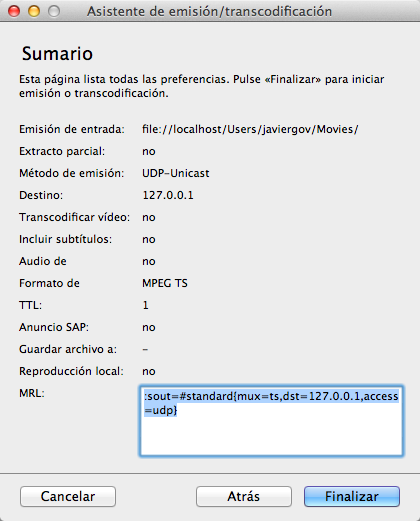
\includegraphics[scale=0.5]{imgs/vlc_transmission.png}
	\caption{Ajustes de la aplicación VLC.app para transmisión de película a través de UDP.}
	\label{vlc_transmission}	
\end{figure}


Considerando las herramientas y el escenario del contenido, la más indicada para transmitir a través de HLS es MediaStream Segmenter ya que puede tomar como entrada el flujo de datos emitidos por UDP y luego entregar su salida a un servidor web Apache que provea a través de internet. De esta forma clientes del tipo iPhone, iPad o Macintosh pueden acceder al contenido multimedia.\\

En la figura \ref{vlc_transmission} se puede observar que la emisión se ha realizado a una ip en específico utilizando el flujo de transporte MPEG2-TS. Este stream se entrega al \textbf{mediastreamsegmenter} con los siguientes parámetros en la línea de comandos.

 \begin{lstlisting}
	mediastreamsegmenter -s 7 -t 11 -D -i ejemplo.m3u8 
	-f ~/Sites/hlsexample 127.0.0.1:1234
\end{lstlisting}

Estos parámetros indican a mediastreamsegmenter que para el ejemplo se genere una lista de reproducción con una ventana de transmisión de \textbf{7} segmentos (\textbf{-s}), los cuales tienen \textbf{11} segundos de duración (\textbf{-t}), además se le indica que los segmentos ya caducados deben ser eliminados (\textbf{-D}). \\

La lista de reproducción lleva el nombre \textit{ejemplo.m3u8} (\textbf{-i}) y los archivos resultantes se deben guardar en el directorio con ruta \textit{$\sim$/Sites/hlsexample} (\textbf{-f}). Por ultimo se indica que la emisión UDP se halla en la dirección ip y puerto: \textit{127.0.0.1:1234}.\\

El resultado de esto es un stream HLS al cual se puede acceder mediante un servidor web como por ejemplo Apache. En caso de este ejemplo los archivos se ubican en el subdirectorio \textit{hlsexample} del directorio asignado a Apache del usuario, para acceder al stream se utilizó un player HTML5 en el archivo \textit{index.html} ubicado junto al resto.

 \begin{lstlisting}
	<html>
	<head></head>
	<body>
		<video src="ejemplo.m3u8" controls 
		autoplay height="360" width="640">
		</video>
	</body>
</html>\end{lstlisting}

Nótese que la fuente al video es la lista de reproducción generada por \textbf{mediastreamsegmenter}, la cual se encuentra en constante actualización mientras la transmisión se lleva a cabo.\\

Ya con el servidor web funcionando, la carga de esta página web permitirá la reproducción del stream en vivo mientras el navegador web sea compatible con el protocolo HTTP Live Streaming utilizando el player HTML5. En la actualidad los únicos navegadores compatibles son Safari y Mobile Safari, desarrollados por Apple.\\
\begin{figure}[H]
	\centering
	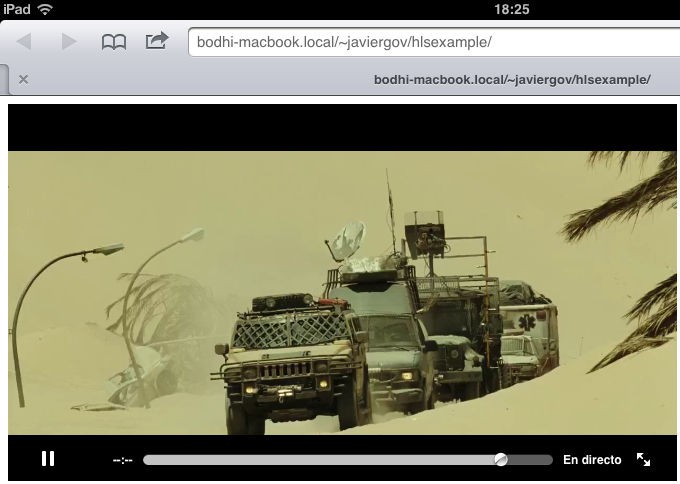
\includegraphics[scale=0.6]{imgs/ipad-hlsexample.png}
	\caption{Captura de pantalla de Mobile Safari en iPad}
	\label{ipad-hlsexample}	
\end{figure}

En la figura \ref{ipad-hlsexample} se puede observar que la reproducción del stream puede ser llevada a cabo por un dispositivo iOS accediendo a la página web creada.\\








	
%	explicar como se probó con resident evil y motorstorm
%	con variantes VOD y live
	
\section{Reproducción y Control de Stream de Video}

%	explicar resumido la estructura como se conecta el server y el cliente, con un  diagrama
	Este trabajo de memoria buscó entregar al usuario control de la linea temporal de un flujo de contenidos en vivo. Para realizar esto se ideó un sistema que intercambia marcas de tiempo entre el cliente y el servidor, de manera que aquel pueda definir desde qué punto el servidor debe crear una lista de reproducción en vivo. \\
	
	Para entregar esta información se utilizó como método de entrada parámetros en la url, que el cliente utiliza para conectarse. Además se puede mejorar la experiencia del usuario indicando al servidor el tipo de enlace que el cliente posee, es decir WiFi o red celular, y expandiendo aun más con un parámetro para definir el canal que se quiere ver, todo desde la misma aplicación.
	
	\subsection{Servidor HTTP}
	El servidor consiste en dos módulos: segmenter y dispatcher, este último depende de los archivos guardados por el segmentador, a su vez el segmentador recibe los datos a través de una emisión UDP o por la entrada estandar \textbf{stdin}.
		\subsubsection{Obtención del Stream}
%		la recepcion de un stream RTMP, codificacion con vlc o ffmpeg y generar un archivo o stream udp
El contenido puede ser obtenido de distintos tipos de fuentes pero este debe cumplir con la especificación de HTTP Live Streaming, es decir entregar al segmentador un flujo de datos codificados con perfiles compatibles con iOS y encapsulados en MPEG2-TS.
		\subsubsection{Sementación del Video}
		% el segmenter que corta su entrada en pedacitos de 10 seg, ademas guarda el tiempo inicial y el final de lo guardado, además se sacarán las fotitos.

El segmentador utilizado fue desarrollado por la empresa AltaVoz S.A. interesada en llevar a cabo el proyecto. Los motivos de este trabajo se deben a que las herramientas dispuestas por Apple funcionan sólamente en versiones recientes del sistema operativo Mac OS X. Al ver esta limitante la empresa se encarga de desarrollar un segmentador que se comporte de forma similar a \textbf{mediastreamsegmenter}, trozando el flujo de entrada en pequeños archivos de cierta duración.\\

 La gran diferencia con el uso de \textbf{mediastreamsegmenter} recalca en el almacenamiento de los archivos resultantes, estos se guardan sin ser eliminados para mantener un gran registro de las transmisiones, el nombre de cada segmento corresponde a la fecha y hora de la recepción de la emisión en formato Unix time (POSIX time) y con extensión \textbf{.ts}. Para mantener orden en el sistema de archivos los segmentos se guardan en subdirectorios por cada hora de contenido, el nombre de estos subdirectorios también llevan Unix time para su catalogación.\\

Una última caracteristica especial del segmentador es marcar el segmento más antiguo y el más reciente en dos archivos \textbf{\textit{start.txt}} y \textbf{\textit{last.txt}} respectivamente, de forma que el cliente pueda representar gráficamente al usuario la disponibilidad de contenido en el \textit{stream}.
		
		\subsubsection{Emisor de la lista de reproducción}
%		dispatcher que recibe epoch, el tipo (canal) y el bwPARAMETER del tipo de enlace Wifi o cellular		
El \textit{Playlist Dispatcher} consiste en un script \textbf{php} disponible en Internet gracias a un servidor web que trabaje con un módulo PHP, el script \textit{playlist dispatcher} debe recibir parámetros del cliente a través de la cadena de consulta (\textit{query string}) de la dirección URL. Los parámetros son los siguientes:

\begin{itemize}
	\item \textbf{t}: Corresponde a la marca de tiempo que el cliente quiere recibir, esta debe ser indicada con el formato Unix Time (POSIX time).
	\item \textbf{s}: Este parámetro indica al script cual contenido entregar a través del stream. Analogamente se puede considerar como el parámetro para definir cual canal de televisión el usuario quiere ver. El valor corresponde a una cadena de caracteres (\textit{string}).
	\item \textbf{c}: Este último parámetro corresponde al tipo de conexión con la cual el cliente está conectado a Internet, pueden ser dos valores, 1 para red celular y 0 para WiFi. Este parámetro se utiliza para optimizar la lista de variantes que entrega el script.
\end{itemize}
		
Con estos parámetros el playlist dispatcher retorna una lista de variantes con referencias a otro script que genera las listas de reproducción (figura \ref{diagramaHLSAltaVoz}).

%aqui poner figura

	\begin{figure}[H]
		\centering
		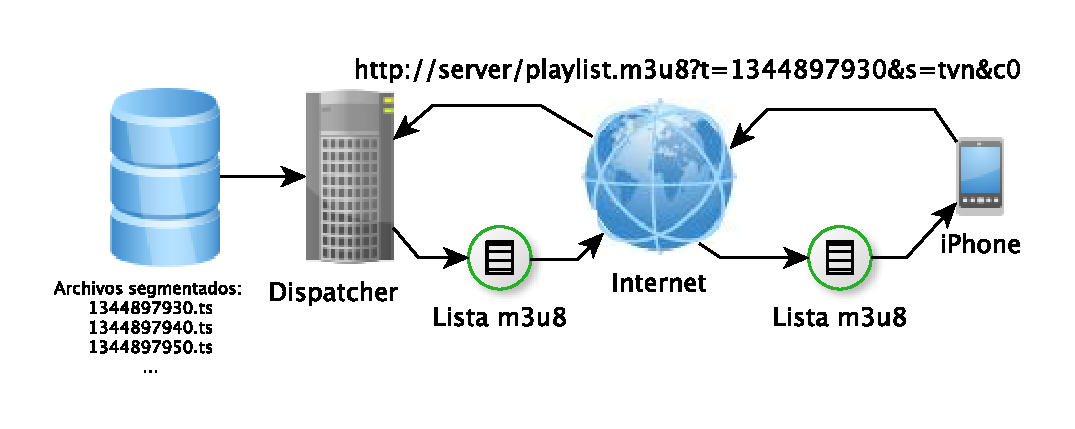
\includegraphics[scale=0.8]{imgs/diagrama-HLS-AltaVoz.eps}
		\caption{Intercambio de información entre Cliente (iPhone) y Servidor (Dispatcher).}
		\label{diagramaHLSAltaVoz}
	\end{figure}		
		
	\subsection{Cliente iOS}
%		descripcion general.
%		como se conecta al server, reachability, entrega a avplayer
Ha de entenderse por cliente una aplicación ejecutada sobre el sistema operativo \textbf{iOS}, su función consiste en mantener un enlace al servidor contactándose directamente con el playlist dispatcher y descargar los segmentos que éste le indique.\\

Además debe presentar en la pantalla del dispositivo el video, o reproducir el audio, según el tipo de stream. Para realizar esto se utilizan componentes de la interfaz de programación de aplicaciones (\textbf{API} - \textit{Application Programming Interface}). El cliente debe permitir al usuario controlar el contenido del stream con una interfaz gráfica simple y precisa.

		\subsubsection{Reproducción con AV Framework}
%		avplayer, playeritem, asset tracks		
Apple en su documentación indica referencias a componentes en iOS que son capaces de reproducir streams HLS, componentes de nivel más alto como por ejemplo un reproductor de video HTML5 anidado en una página web o la clase \textbf{MPMoviePlayerViewController} que pertenece a \textbf{Media Player Framework}, la que consiste en una pantalla que incorpora controles como barras deslizables para video y botones de control, facilitando de gran manera a los desarrolladores presentar contenidos multimedia. \\

Sin embargo como este trabajo buscó presentar una característica nueva a lo que es la reproducción de streams, se debió desarrollar un componente que se asemeje al estándar MPMoviePlayerViewController (figura \ref{IMG-mpmpvc-example}) incluyendo la característica de control de contenido y compartir información a través de Twitter.\\

Uno de los componentes que significó una gran ayuda en el desarrollo del cliente es \textit{AV Foundation Framework}, la cual es una estructura de más bajo nivel que \textbf{Media Player Framework}. 
En la figura \ref{IMG-ios-tech-frameworks} se interpreta que los módulos de AV Foundation se encuentran bajo \textbf{UIKit}, el cual es la infraestructura para interfaces gráficas en iOS, por lo tanto al utilizar AV Foundation para reproducir contenido temporal del tipo audio o video es necesario implementar con los componentes de UIKit la salida gráfica para el usuario.\\

El motivo de utilizar AV Foundation, además de una interfaz gráfica personalizada, es la obtención de datos que las clases por defecto no entregan, datos que están relacionadas con el control personalizado de la reproducción.

% y que permite obtener mayor información de los componentes de un archivo o stream multimedia.

% imagen
\begin{figure}[H]
	\centering
	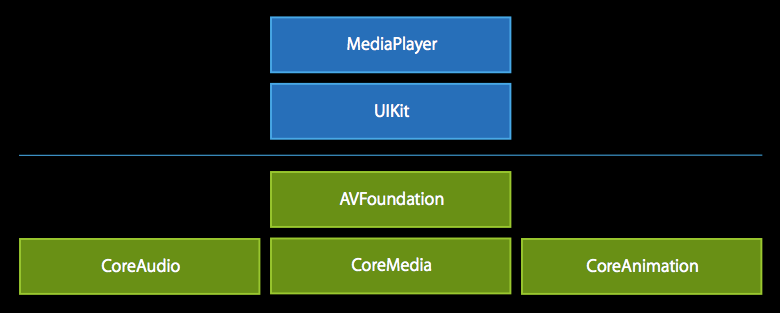
\includegraphics[scale=0.5]{imgs/ios-tech-frameworks.png}
	\caption{Infraestructuras tecnológicas para el manejo de multimedia en iOS}
	\label{IMG-ios-tech-frameworks}	
\end{figure}

% imagen
\begin{figure}[H]
	\centering
	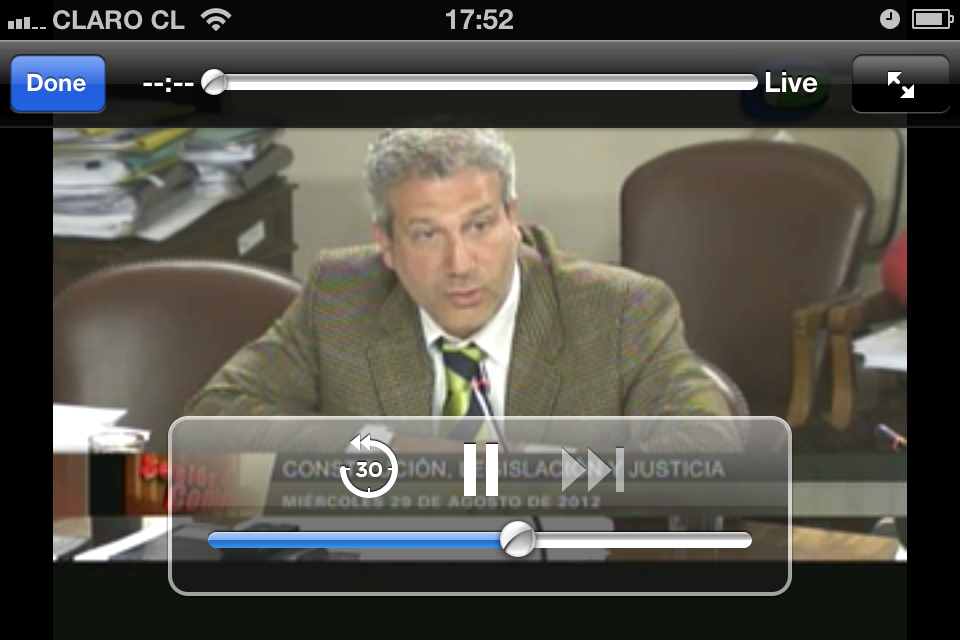
\includegraphics[scale=0.3]{imgs/mpmpvc-example.png}
	\caption{Aplicación reproduciendo stream HLS con MPMoviePlayerViewController}
	\label{IMG-mpmpvc-example}	
\end{figure}

		\subsubsection{Recopilación de datos del Stream}
%		kvo, notificaciones, periodic observers, la fecha y que se hace con ella
Utilizando observadores de notificaciones centralizadas (\textit{Notification Center} \cite{bib:ios-nsnotificationcenter}), observadores de cambio de valor (KVO - \textit{Key Value Observing} \cite{bib:kvo-guide}) y observadores periódicos (\textit{Periodic Observers} \cite{bib:avplayer-periodic}), es posible llevar un registro del contenido del stream, como también la mayoría de los cambios de estado del reproductor.\\

Para mantener de forma continua la información temporal del stream se han asociado a la instancia de la clase AVPlayer dedicada a la reproducción del stream entregado por URL, los siguientes datos.\\
% enumerar los datos obtenidos

\textbf{Revisión periódica}:

\begin{enumerate}
\item \textbf{Tiempo de reproducción}: Este se supervisa en un intervalo de 1/10 de segundo de forma que con esta razón de cambio la interfaz gráfica se actualice, se ajusta a  este valor de tiempo (100 ms) de forma que el usuario no identifique irregularidad en el temporizador y a la vez la carga en ciclos de ejecución no afecte el desempeño de la máquina.
\item \textbf{Fecha asociada al stream}: Este valor es parte fundamental en el funcionamiento del stream con saltos en el tiempo, su origen se debe al tag asociado a la lista de reproducción del stream.
\label{observer-date}
% esto no está en la memoria, se hizo después para Janus.
%\item \textbf{Tasa de Bits}: Se obtiene el valor de la tasa de bits promedio del flujo de datos multimedia, para obtenerlo se deben separan los activos (AVAssets) del item (AVPlayerItem) en reproducción. 

\end{enumerate}

En el caso de la observación periódica de datos, esta se debe detener previamente al termino de la reproducción de cierto stream, debido a que se debe liberar de memoria el reproductor y estos observadores retienen en memoria al reproductor. En caso que no se siga esta sugerencia, al iniciar una nueva reproducción los observadores utilizados anteriormente se vuelven a crear causando duplicidad y por ende pérdida de memoria.\\


\textbf{Notificación en base a cambios}:

La mayoría de los valores observados sirven como guía para controlar el funcionamiento del reproductor. En caso de cualquier cambio en el estado de los atributos observados se dispara una notificación desde el objeto con el cambio con destino al observador asociado. 
En el desarrollo de esta aplicación la clase encargada de gestionar la interfaz gráfica de los objetos (\textit{View Controller}) actúa también como observador.\\

Un ejemplo de observación por cambio de valor (\textbf{KVO}) se muestra en la figura \ref{exampleCodeObserver}, donde \textit{player} es el objeto, \textit{self} es la instancia del \textit{ViewController} que recibirá los avisos de cambio, y \textit{rate} es el atributo a indagar. Además se pueden ajustar opciones adicionales para la recepción de las notificaciones y asociar un contexto a la notificación. De esta forma cuando el valor de \textit{rate} en el reproductor \textit{player} cambie, ya sea por algún evento en la transmisión o alguna interacción por parte del usuario, se notificará al \textit{ViewController} para tomar curso de acción.
\begin{figure}[H]
	\centering
	\begin{lstlisting}
	[player addObserver:self  
			 forKeyPath:@"rate"
		        options:NSKeyValueObservingOptionNew
		        context:TracksChangeContext];
	\end{lstlisting}
	\caption{Ejemplo de objeto Reproductor siendo asociado un observador su atributo \textit{rate}}
	\label{exampleCodeObserver}	
\end{figure}	
 
 
 Teniendo claro el sistema de observación de instancias, se explican a continuación los campos de interés para este proyecto:
\begin{itemize}
\item \textbf{Estado}: El atributo \textit{status} de la clase AVPlayer es del tipo sólo-lectura e indica si la instancia de AVPlayer es capaz de reproducir el flujo multimedia. Este atributo puede tener tres valores del tipo integer: \textit{AVPlayerStatusUnknown}, \textit{AVPlayerStatusReadyToPlay} y \textit{AVPlayerStatusFailed}.

\item \textbf{Razón de reproducción}: Consiste en un valor flotante en el rango entre 0.0 y 1.0. El atributo rate indica si el audio y/o video se reproduce a velocidad normal (1.0) o se encuentra detenido (0.0). Valores intermedios se asocian a una menor velocidad de reproducción, en el caso de este proyecto no se buscó entregar un control de velocidad de reproducción al usuario fuera de la normal. También se debe tener en cuenta que este atributo se puede ajustar por instrucciones externas.

\item \textbf{Búfer de Datos}: El reproductor AVPlayer posee un atributo que es una instancia de AVPlayerItem, esta clase es una abstracción del flujo de datos \textit{currentItem}. Tomando en cuenta esto se deben observar tres propiedades de este \textit{currentItem}, estas son: 
\begin{itemize}
\item \textit{playbackBufferEmpty}
\item \textit{playbackLikelyToKeepUp}
\item \textit{playbackBufferFull}
\end{itemize}
Ellas gatillan notificaciones al cambiar su valor BOOL a verdadero para informar a las otras clases y tomar curso de acción. Por ejemplo al recibir una notificación de buffer vacío, es necesario avisar al usuario con una representación gráfica del reproductor mientras carga.

\item \textbf{Pistas de medios}: Debido a que el flujo de datos puede solamente audio, o video y audio. Es necesario supervisar el tipo de medio que se está presentando. Para esto se utiliza el atributo \textit{tracks} del flujo de datos (\textit{currentItem}). Este atributo consiste en un arreglo (NSArray) de instancias de AVPlayerItemTrack, clase que representa cada pista multimedia del flujo de datos, cada pista puede ser texto (AVMediaCharacteristicLegible), audio (AVMediaCharacteristicAudible) o video (AVMediaCharacteristicVisual). Observando el cambio de componentes en el flujo es posible adecuar el reproductor según el tipo de medio que se presenta al usuario.

\item \textbf{Rango de reproducción}: \textit{seekableTimeRanges} se refiere al atributo asociado a la disponibilidad temporal del item en reproducción, el rango donde es posible realizar búsqueda de cuadros de reproducción. Este valor cambia constantemente debido a que el contenido recibido por HTTP Live Streaming se encuentra en actualización permanente guardando tiempo adicional para reproducción. Este atributo se observa con el fin de rastrear si se están obteniendo segmentos del contenido.
% StreamPlayerVC.m: 748 start: 630.415833, duration: -15.000000
\end{itemize}
\label{item:seekableTimeRanges}
\label{item:kvo-tracks}
		
\subsection{Intercambio de información entre componentes}
\label{subsec:cookies}
%	conexión, envio de epoch, recepcion de m3u8, start y last txt	

Se debe considerar que el intercambio de información se realiza entre el dispatcher y la aplicación cliente como se muestra en la figura \ref{diagramaGral}. Para esto se insta usar el reproductor de clase AVPlayer mediante su método de inicialización:

\textit{initWithURL:(\textbf{NSURL} *)url}, que toma como argumento un URL al dispatcher con los parámetros explicados anteriormente. Luego que el reproductor se ha iniciado, se procede a asociar los observadores a la instancia para luego llamar a la reproducción.\\

% cookies ref: http://es.wikipedia.org/wiki/Cookie_(informática)
El método de inicialización se basa en una petición HTTP. La administración de datos de usuario en el cliente (\textit{cookies}) son establecidos por el servidor y el sistema del cliente (iOS) se encarga de devolver la información con cada petición. Esto simplifica de gran manera cada nuevo enlace que la aplicación cliente debe hacer, liberando la carga a solamente establecer las nuevas URLS.

Por el lado del servidor, aparte de los campos en la cadena de consulta (\textit{query string}), se establece cada conexión utilizando las siguientes cookies:

\begin{itemize}
\item \textbf{t0}: Tiempo pedido en el parámetro t, de la cadena de consulta.
\item \textbf{tp}: Tiempo actual de ejecución del script en el servidor.
\item \textbf{si}: Secuencia inicial de la lista de reproducción HLS.
\item \textbf{sf}: Secuencia final de la lista de reproducción HLS.
\item \textbf{ti}: Tiempo inicial encontrado en los archivos, corresponde a la marca de tiempo más cercana al valor de t0, ya que puede ocurrir que el tiempo pedido no coincida con el nombre de archivo de los segmentos.
\item \textbf{tl}: Tiempo del ultimo segmento de la lista de reproducción HLS.

\end{itemize}
 
En la programación del cliente no se realizó tarea alguna respecto a cookies, el sistema operativo iOS se encargó de establecer y responder los valores de estas cookies según lo pedido por el servidor. Esta simpleza se debe gracias a las restricciones puestas por Apple en sus frameworks multimedia, limitando las inicializaciones a solo URL como argumentos en vez de instancias configuradas de \textit{NSURLRequest}. 
Los métodos que establecen conexiones incluyen un atributo \textit{NSHTTPCookieAcceptPolicy} con el valor por defecto \textit{NSHTTPCookieAcceptPolicyAlways}, es decir siempre están dispuestos a aceptar y almacenar cookies. \\

Con todos estos valores el servidor calcula y contesta al cliente un stream HLS con los segmentos apropiados a la reproducción.
	
	
\clearpage
\section{Interfaz Gráfica}

Si la aplicación ya es capaz de pedir y recibir un flujo de datos multimedia por HTTP Live Streaming, es tarea del cliente mostrar el contenido ya sea video y/o audio. La versatilidad de los dispositivos iOS permiten variadas formas de entregar la información al usuario, sin embargo Apple se mantiene sobre-protector respecto al diseño funcional de las aplicaciones con documentos guía que hacen a la vez de pauta en el proceso de evaluación de aplicaciones para ser ingresadas a la App Store.

  \subsection{Directrices de diseño de Apple}
% http://developer.apple.com/library/ios/#documentation/UserExperience/Conceptual/MobileHIG/Introduction/Introduction.html 
%		las guias de diseño y recomendaciones de apple

Las Directrices de interfaz humana de iOS (\textit{iOS Human Interface Guidelines}) describen los principios que ayudan a diseñar una interfaz y experiencia de usuario para las aplicaciones iOS.\\

Estas guías no describen los diseños en código, abarcan convenciones como características de la plataforma, casos de transición entre pantallas, gestos que el usuario espera y tecnologías de comunicación entre componentes.
Para desarrollar la aplicación se revisaron puntos de estas guías con tal de obtener un producto acorde a lo esperado por los usuarios de iOS. No se quiso innovar en materia de controles y gestos, por lo tanto se utilizaron componentes estándar del framework UIKit.
	
	\subsection{Componentes de UIKit}
	Para el desarrollo de la aplicación cliente se utilizaron recursos dispuestos en el framework UIKit con tal de mantener la percepción del usuario con la interfaz gráfica respecto al resto de las aplicaciones que ejecuta en su sistema. El mayor cambio respecto al los componentes comunes de la interfaz fue en el selector de segundos debido a que la selección de fecha no abarca totalmente lo requerido por el sistema diseñado.
	
		\subsubsection{UIDatePicker}
		\label{subsec:datepicker}
% 	foto, como se usa, el hack para horizontal
Para el trato de valores de fechas, el framework de interfaz gráfica UIKit pone a disposición la clase UIDatePicker, que presenta en pantalla una rueda con distintas secciones asociadas a cierta fecha con la que se ajuste. Además permite llamar métodos al seleccionar una fecha en particular. Sin embargo este control no permite seleccionar una fecha especificándola desde el año hasta los segundos, permite especificar sólo hasta los minutos. \\

Para solucionar esto se ideó un control personalizado que presenta una rueda extra con valores de 0 a 59 que se adicionan a los minutos seleccionados con el UIDatePicker. Esta rueda especial es una modificación de la clase UIPicker de propósito más general, se transformó su dibujo rotando en 90º gracias a la API Core Graphics Framework. 

\begin{figure}[H]
	\centering
	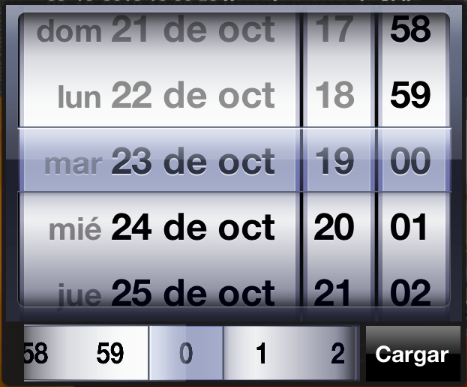
\includegraphics[scale=0.5]{imgs/datepicker-mod.png}
	\caption{Control del tiempo de la transmisión, UIDatePicker y UIPicker modificado}
	\label{datepicker-mod}	
\end{figure}
 
		\subsubsection{UIButton}
		El reproductor presenta botones de control de reproducción en base a un reproductor estándar de MPMoviePlayerViewController, estos son PLAY/PAUSE, Next. Estos botones son lo único que comparten con un reproductor normal ya que además se debe incorporar un botón para compartir el momento de la reproducción a través de redes sociales. Se agrega entonces un botón con el icono de twitter que presenta un formulario de acción con ítems para cerrar la sesión, compartir en twitter o cancelar la acción de compartir.
		
%				play pausa, ibactions
		\subsubsection{Volume Slider}

		Para presentar el control de volumen se utilizó una clase estándar del sistema operativo, llamada MPVolumeslider, encargada de presentar un deslizador que está directamente relacionado con los botones del hardware de los dispositivos iOS. Tanto así, que en materia de depuración (\textit{debug}), el simulador no permite mostrar en pantalla dicho control. Se agrega ajustando un rectangulo destinado como perimetro para que el sistema presente dicho control en una subvista.
		
		\subsubsection{Vistas de Tablas}
%		volumen, slider de view controller tipo facebook, etc
Para representar el cliente de twitter se utilizó una instancia de la clase UITableView, clase que tiene como fin presentar y editar listas jerárquicas de información. La información se obtiene del resultado de una llamada a twitter utilizando su API de búsqueda. El resultado consiste en un archivo JSON (\textit{JavaScript Object Notation}) que contiene los tweets de los últimos 6 a 9 días respecto a la consulta realizada. Para el caso de esta aplicación, se utiliza el hashtag \textbf{\#SocialStream} como se puede ver en la figura \ref{sshot-twitterclientvc}.\\

Para poder presentar la tabla sin perder parte de la transmisión se muestra el cliente de twitter bajo la vista del reproductor. Utilizando la clase ZUUIRevealController fue posible apilar en pantalla dos controladores de vista: TwitterClientVC y StreamPlayerVC. Para lograr presentar el controlador de vista inferior, fue necesario asociar a la vista del reproductor un botón que permita arrastrar con el dedo o desplazar con un toque la vista que lo posee. Esto se realizó asociando la acción de tocar dentro del botón y el gesto \textit{navigationBarPanGestureRecognizer} a la barra que lo contiene. El método asociado \textit{revealToggle:} de la instancia de ZUUIRevealController permite mostrar, ocultar o arrastrar las vistas superpuestas. En la figura \ref{sshot-twitterclientvc} se muestra el instante donde el usuario arrastra la vista del reproductor a través del botón \textbf{Twitter}.


\begin{figure}[H]
	\centering
	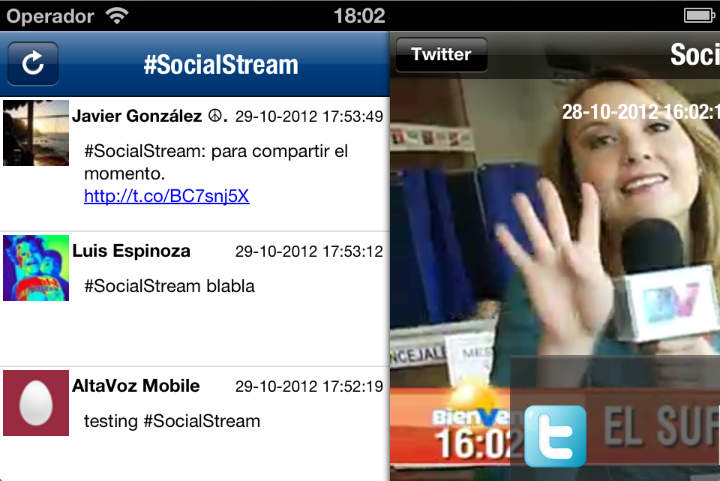
\includegraphics[scale=0.4]{imgs/sshot-twitterclientvc.png}
	\caption{Revelación del cliente de Twitter en base a UITableView}	
	\label{sshot-twitterclientvc}
\end{figure}
 
 
%\clearpage
\section{Integración Redes Sociales}
	%diagrama de como funciona el posteo y recepcion de twitts
	Para destacar la connotación de carácter social de la aplicación, se incorporó un sistema de compartimiento en base a la red social Twitter. Este sistema no se limita solamente a esta red social, es posible incorporar otras, sólo que se utilizó ésta como ejemplo.\\
	
	En resumen, el usuario al pulsar el botón \textbf{\textquotedblleft t\textquotedblright} visible en la imagen \ref{sshot-twitterclientvc} genera un URL en base a la fecha de la transmisión que está viendo, este URL se comprime a través del servicio bit.ly con tal de aminorar la cantidad de caracteres en el mensaje y luego se entrega al usuario en un campo de texto donde se le permite describir lo que comparte. Una vez en la red Twitter, usuarios que observen este mensaje a través de la misma aplicación pueden llegar a reproducir el instante compartido por el autor del mensaje (figura \ref{diagramaTwitterShare}).
	
	%insertar imagen del sistema
	\begin{figure}[H]
		\centering
		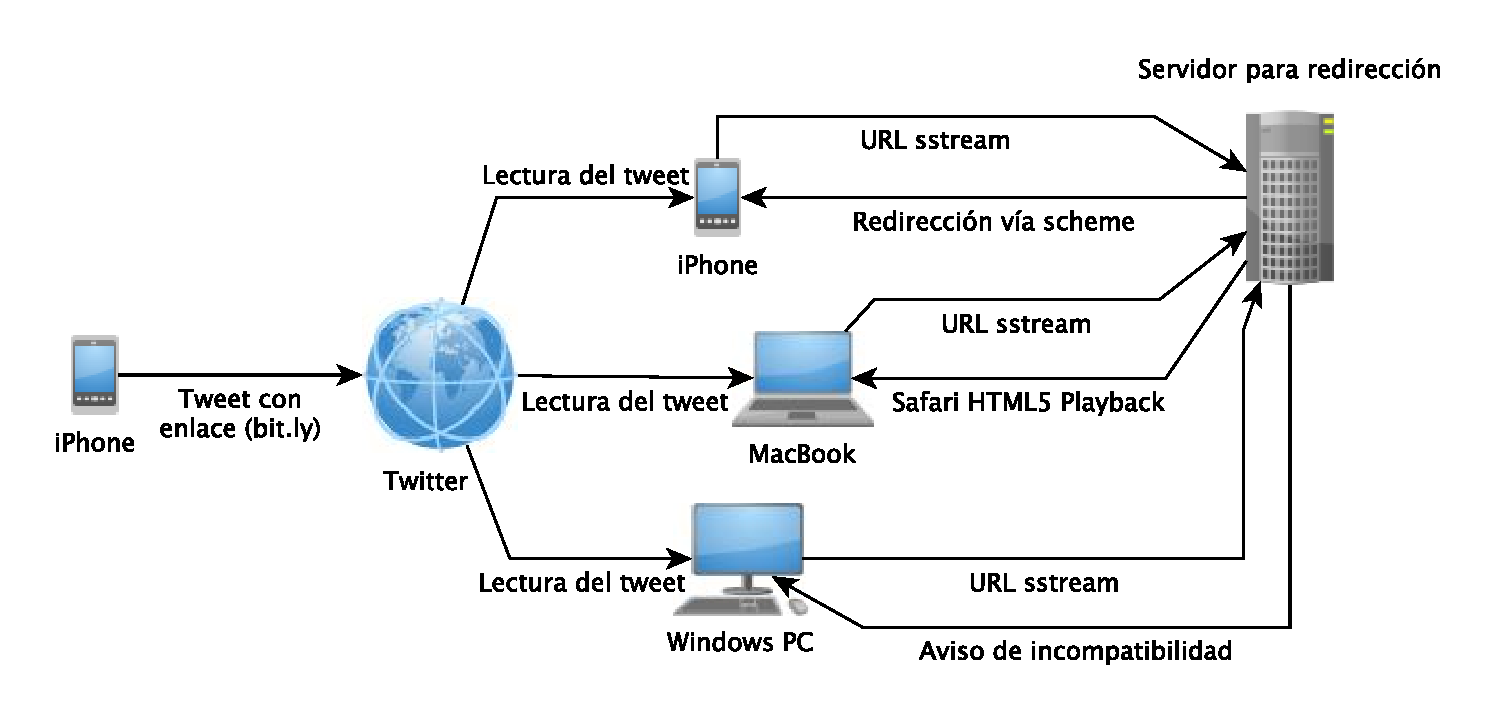
\includegraphics[scale=0.6]{imgs/twitter-share-diagram.eps}
		\caption{Flujo de enlaces compartidos a través de Twitter.}
		\label{diagramaTwitterShare}
	\end{figure}		
	
	\subsection{Twitter}
	%http://www.alexa.com/siteinfo/twitter.com
	La red de microblogging Twitter permite difundir mensajes de forma pública y también privada a millones de usuarios en internet, siendo uno los sitios más populares de la web\cite{alexa-twitter} permitiendo que personas no suscritas puedan ver los mensajes.
	La limitante de cada mensaje se reduce a 140 caracteres, más que suficientes para difundir enlaces desde la aplicación desarrollada y permitiendo además una pequeña descripción por parte del usuario.
		\subsubsection{API Twitter}
		Para la muestra de los mensajes compartidos, se utilizó \textit{Twitter Search API}, interfaz dedicada a búsquedas en el índice de mensajes (\textit{tweets}) en tiempo real. Esta se caracteriza por lo siguiente:
		
		\begin{itemize}
		\item Su historial dura no más de una semana, el indice de mensajes abarca entre 6 a 9 días.
		\item La búsqueda no requiere de autenticación, se realiza anónimamente.
		\item El resultado de la búsqueda se basa en relevancia del tema en vez de la totalidad de sus mensajes. Esto debido a las políticas del servicio de Twitter donde se privilegia el alcance de los mensajes según la reputación de los usuarios \cite{twitter-relevance}.
		\end{itemize}

Tomando en cuenta estos puntos Search API satisface la obtención de mensajes compartidos desde la aplicación cliente, si bien existen alternativas dispuestas por twitter para la obtención de mensajes, no significan una mejora respecto al fin de la aplicación cliente. Se prefiere por su simpleza.
		
%		las llamadas de twitter que se utilizarán
		\subsubsection{Sharekit vs. Twitter Framework}
%		el porqué se utilizó sharekit en vez de twitter framework, el argumento de las apps de twitter
Durante el desarrollo de la aplicación cliente Apple Inc. lanzó al público el sistema operativo iOS 5, el cual permite entre muchas características, la integración del sistema con la red social Twitter mediante \textbf{Twitter.framework} . Por simpleza y compatibilidad con versiones anteriores de iOS se descartó utilizar esta nueva herramienta para utilizar la biblioteca de código libre \textbf{Sharekit}\cite{library-sharekit}, destinada a integrar todo tipo de redes sociales incluyendo twitter. Otro motivo de esto es la posibilidad de expandir a otras redes el contenido que se comparte a través de la aplicación cliente. \\

En caso que se desee, es posible utilizando Sharekit modificar el mensaje a compartir de forma que el usuario no elimine el URL relacionado al contenido compartido.

		\subsubsection{Post en Twitter}
%		como postear en twitter desde la app, action sheet
		Para entregar el momento que se está viendo u oyendo, es necesario tener la fecha de la transmisión, esto se obtiene de uno de los observadores periódicos encargados de la fecha del flujo de datos (\ref{observer-date}). El objeto obtenido es una instancia de la clase \textbf{NSDate}, encargada de registrar información temporal, convenientemente se utiliza el método de la clase: \textit{\textbf{timeIntervalSince1970}} que entrega la cantidad de segundos entre el 1 de enero de 1970 y la fecha en cuestión, el valor obtenido es del tipo \textbf{\textit{double}} por lo tanto es necesario convertir el valor a NSString, cadena de caracteres. Una vez generado el URL con el valor temporal en su cadena de consultas se procede a un campo de texto que incluye el URL, de manera que el usuario agregue algún comentario y dé la instrucción de enviar si lo desea.
		
		
		En caso de no tener el valor para la fecha en reproducción la aplicación no permite compartir.

		\subsubsection{Seguimiento de Hashtag}
		%las llamadas de url para el cliente de twitter
		Para realizar el seguimiento de los mensajes se utilizó Search API como se explicó anteriormente. Para realizar la llamada se realiza una conexión con el URL: 
\url{http://search.twitter.com/search.json?include_entities=true&q=%23SocialStream} \\
		
		Nótese que el último componente del URL corresponde al hashtag, o marca de seguimiento que se se utiliza en los mensajes. La respuesta por parte de Twitter es un objeto del tipo JSON que contiene un arreglo con los mensajes resultantes.

\begin{figure}[H]
	\centering
	\begin{lstlisting}
"created_at": "Thu, 08 Nov 2012 21:21:59 +0000",
"entities": {
    "hashtags": [
    		{ "indices": [ 0, 13 ], 
    		  "text": "SocialStream" }],
    "urls": [
        { "display_url": "bit.ly/SPCO4a",
            "expanded_url": "http://bit.ly/SPCO4a",
            "indices": [ 30, 50 ],
            "url": "http://t.co/uKm7VRMb" } ],
    "user_mentions": [] 
    },
"from_user": "javiergov",
"from_user_id": 76853723,
"from_user_id_str": "76853723",
"from_user_name": "Javier Gonzalez O.",
"geo": null,
"id": 266651804614418430,
"id_str": "266651804614418432",
"iso_language_code": "en",
"metadata": { "result_type": "recent" },
"profile_image_url": "http://url.del.avatar/foto.jpg",
"source": "&lt;a href=&quot;http://sitio.dela.app&quot;
					&gt;SocialStream for iOS&lt;/a&gt;",
"text": 
"#SocialStream http://t.co/uKm7VRMb texto del tweet",
"to_user_id": 0,
"to_user_id_str": "0",
        	\end{lstlisting}
	\caption{Componentes de un Tweet, respuesta de Twitter Search API}
	\label{tweet-json}	
\end{figure}			

		
		\subsubsection{Extracción de información de un Tweet}
%		como se parseó el json con los twitts y saber si eran sstream
Para presentar los mensajes de forma simple para el usuario fue necesario serializar el objeto JSON obtenido de Search API. Gracias al componente \textbf{NSJSONSerialization} del entorno de desarrollo de iOS, como se muestra en \ref{json-serialization}, es posible generar un objeto del tipo NSDictionary para ser entregada a la clase encargada de generar la tabla con los mensajes.

\begin{figure}[H]
	\centering
\begin{lstlisting}
NSError *error = nil;
NSDictionary *dict =
[NSJSONSerialization 
		JSONObjectWithData:responseData 
				   options:NSJSONReadingMutableLeaves
                   	 error:&error];
if (error) 
 MLogString(@"serialization error: %@",
 					[error description]);
\end{lstlisting}
	\caption{Obtención de los datos desde JSON mediante NSJSONSerialization}
	\label{json-serialization}
\end{figure}	

Una instancia de NSDictionary posee una cadena de claves y valores asociados, la generada del objeto JSON entrega valores de las claves encontradas en la figura \ref{tweet-json}.
Para presentar el contenido en la tabla de la interfaz gráfica se utilizaron los valores de las claves:
\begin{itemize}
\item \textbf{\textquotedblleft from\_user\_name"}: (línea 16) El nombre completo del usuario.
\item \textbf{\textquotedblleft text"}: (línea 25) El cuerpo del mensaje.
\item \textbf{\textquotedblleft profile\_image\_url"}: (línea 22) La dirección a la imagen que el usuario utiliza como avatar.
\item \textbf{\textquotedblleft created\_at"}: (línea 1) La fecha en que se realizó el tweet, tomar en cuenta que no corresponde a la fecha de la transmisión que el usuario comparte. 
\end{itemize}
Al pulsar en algún mensaje representado en la tabla \ref{sshot-twitterclientvc}, se utiliza el valor de la clave \textit{\textbf{\textquotedblleft expanded\_url"}} (\ref{tweet-json}, línea 8) para analizar si su contenido es utilizable por la aplicación.

	\subsection{Bit.ly}
%		desmenuzar el enlace de bitly
Para entregar una buena experiencia al usuario se utilizó el servicio de compresión de URL \textbf{Bit.ly}, de forma que el enlace al stream (que además incluye marca de tiempo) no utilice demasiados caracteres. El motivo es la limitante de twitter de 140 caracteres por mensaje, los cuales la aplicación debe utilizar lo mínimo para compartir.\\

Otra característica útil para la supervisión de la aplicación y el servicio \textit{SocialStream} en su totalidad, es la posibilidad de utilizar las llamadas a la API de Bit.ly junto a las credenciales de una cuenta previamente hecha para llevar un registro del uso de los enlaces. \\

La compresión se debe realizar al compartir en twitter un enlace al stream, y descompresión cuando el usuario pulsa en un tweet de la tabla (figura \ref{sshot-twitterclientvc}).

		\subsubsection{API Bit.ly}
%		las llamadas de la api que se utilizaron
%		http://dev.bitly.com/api.html

Para utilizar y mantener el registro de los enlaces compartidos, se configuran credenciales obtenidas del sitio web \cite{bitly-settings} (nombre de usuario y Legacy API Key) en un archivo de cabecera de la biblioteca Sharekit.


		
		\subsubsection{Compresión de URL}
Para comprimir un URL se realiza una petición al servidor con el comando \textit{\textbf{shorten}} utilizando el URL que se muestra en la figura \ref{bitly-shorten} y con argumentos en la cadena de consulta para los campos: login, apikey, longUrl y format.

\begin{figure}[H]
	\centering
\begin{lstlisting}
http://api.bit.ly/v3/shorten?
					login=usuario
					&apikey=R_1234567890
					&longUrl=http%3A%2F%2Fgoogle.com%2F
					&format=txt
\end{lstlisting}
	\caption{Ejemplo de URL para compresión con Bit.ly API}
	\label{bitly-shorten}
\end{figure}	

La respuesta entregada depende del campo \textit{format} especificado en la cadena de consulta. En el ejemplo de la figura \ref{bitly-shorten} se espera en formato de texto plano, en caso de no definir formato la respuesta se entrega como objeto JSON.\\

Para una respuesta exitosa se recibe una cadena de caracteres con el URL comprimido de tipo 
\textbf{http://bit.ly/\textless hash comprimido\textgreater} \\

En caso de cualquier falla, el texto entregado es la causal misma del error, por lo tanto cual sea la respuesta debe ser analizada su integridad como URL antes de ser entregada al resto de las instancias de las clases que componen la aplicación. Esta comprobación se realiza comparando el \textit{scheme} del \textbf{NSURL} creado a partir del texto resultante, en caso de ser \textbf{http} o \textbf{https} se considera conforme por parte de la aplicación.\\ 

Algunas respuestas erróneas pueden ser:
\begin{itemize}
\item INVALID\_APIKEY: Clave para acceder a la API es inválida o no concuerda con el usuario. 
\item INVALID\_LOGIN: El nombre de usuario no corresponde a la clave de API o no existe.
\item INVALID\_ARG\_FORMAT: El formato requerido no corresponde a los dispuestos a entregar por Bit.ly, los cuales son txt, json o xml.
\item INVALID\_URI: El recurso a comprimir no se entrega codificado en código porciento\cite{percent-encoding}.
\end{itemize}

		\subsubsection{Expansión de atajo bit.ly}
%		como se expande un url de bitly y se usa en la app
Para expandir un URL comprimido por Bit.ly se utiliza la llamada a la API de forma similar al método de compresión, se diferencia con el comando \textit{\textbf{expand}} en vez de \textit{shorten} y entregando el hash comprimido del enlace corto obtenido del valor de la clave \textit{\textbf{\textquotedblleft expanded\_url"}} incluido en un tweet (\ref{tweet-json}, línea 8). El hash comprimido corresponde a la ruta del URL.

\begin{figure}[H]
	\centering
\begin{lstlisting}
http://api.bit.ly/v3/expand?
						login=usuario
						&apikey=R_1234567890
						&hash=WQfFTO
\end{lstlisting}
	\caption{Ejemplo de URL para expandir hash comprimido perteneciente a un URL Bit.ly}
	\label{bitly-expand}
\end{figure}	
Nótese que en el URL de la figura \ref{bitly-expand} no especifica formato de respuesta, por lo tanto se recibe por defecto un objeto JSON. El motivo de este cambio es sólo de investigación, ya que de esta forma se puede obtener mayor información que una respuesta de sólo texto.

\begin{figure}[H]
	\centering
\begin{lstlisting}
{   "data": {
        "expand": [
            { 	"global_hash": "900913",
                "hash": "WQfFTO",
                "long_url": "http://google.com/",
                "user_hash": "WQfFTO" }]},
    "status_code": 200,
    "status_txt": "OK" }
\end{lstlisting}
	\caption{Respuesta exitosa de tipo JSON al expandir URL Bit.ly}
	\label{bitly-json-response}
\end{figure}	
Los datos del resultado de la llamada se entregan a una instancia de NSJSONSerialization con el mismo método utilizado para desmenuzar la información de los tweets (figura \ref{json-serialization}). De esta forma se obtiene un objeto del tipo NSDictionary y para luego fácilmente obtener el valor asociado a la clave \textbf{\textquotedblleft long\_url"}.
En caso de obtener como respuesta un error los datos serán de igual forma del tipo JSON, sólo que la información de la clave \textbf{\textquotedblleft status\_txt"} corresponderá a la causa del error en vez del OK que se obtiene al realizar una operación exitosa (figura \ref{bitly-json-response}). El valor de las causas de error son las mismas que las indicadas anteriormente.

%NOT_FOUND
		\subsubsection{Seguimiento de un Hipervínculo}		
%		como se monitorean los twitts por bitly y se puede usar pa marketing, saber que es lo popular etc		
El hecho de entregar las credenciales de una cuenta al comprimir y expandir URL con Bit.ly permite monitorear los enlaces compartidos y la cantidad de aperturas que estos tienen. Esta información puede ser de gran ayuda para identificar qué programas o secciones transmitidas en la señal son más populares, de forma similar a lo que es el \textit{\textquotedblleft people meter"} o rating en la televisión abierta.

Esta información se encuentra en \textbf{\url{https://bitly.com/a/stats}} donde es necesario acceder con las mismas credenciales configuradas en la aplicación.

\clearpage
\section{Registro en iOS}
El sistema operativo iOS permite registrar \textit{schemes}, con lo cual el sistema reconoce qué aplicación debe encargarse de interpretar cierto URL. Esta característica es aprovechada por la aplicación cliente de forma que los enlaces compartidos por los usuarios en Twitter lleven a la aplicación cliente sin que esté necesariamente en ejecución.
	\subsection{Schemes}
%	explicar que son los schemes
	Un \textbf{\textit{Scheme}} es el prefijo de un \textit{Universal Resource Locator} (\textbf{URL}), el cual define el protocolo a utilizar para ubicar un recurso.
	Es necesario además que se pueda acceder al contenido compartido a través de la Web o incluso desde otras aplicaciones del sistema.

Para esto es necesario que la aplicación indique en su archivo de información general \textbf{\textquotedblleft info.plist\textquotedblright}  \ los schemes de los URL que tiene interés.
En el caso de la aplicación cliente, se registra un scheme como \textquotedblleft socialstream\textquotedblright , de manera que URLS de la forma \textbf{\url{socialstream://www.ejemplo.com/}} sean entregados a la aplicación cliente.

% http://developer.apple.com/library/ios/documentation/iPhone/Conceptual/iPhoneOSProgrammingGuide/AdvancedAppTricks/AdvancedAppTricks.html#//apple_ref/doc/uid/TP40007072-CH7-SW50

	\subsection{Redireccionamiento vía Web}
%	explicar breve como funcionará la carga del scheme sstream, en web y mobile
La forma más simple que se ideó para entregar la información, según las variadas plataformas que se conectan a internet, consiste en comunicar a través de la herramienta común que poseen los móviles y computadores: el navegador web.\\

El navegador web al iniciar la conexión través del protocolo HTTP con cierta página remota entrega dentro de sus cabeceras el Agente de Usuario \textit{(user agent)}, con lo cual es posible identificar qué cliente se conecta y a la vez personalizar el contenido a entregarle.

		\subsubsection{PHP Script}
		\label{subsec:php-redir}
%		explicar brevemente el script php 
Se desarrolló un script en PHP encargado de identificar el cliente que se está conectando al servidor del stream, y según el tipo de dispositivo o navegador redirecciona a un URL con scheme personalizado, o presenta una página web con información a social stream.\\

El acceso al script requiere, para su buen funcionamiento, ciertos campos como mínimo relacionados con la transmisión que se compartió y se incluyen en el URL, como query strings (cadena de consulta), estos son el tipo de canal y la marca de tiempo, similares a los entregados al dispatcher por parte del cliente se hace una petición de lista de reproducción.
El script se encarga de analizar las marcas de tiempo y tipo de señal para entregar un URL especial según el agente de usuario del cliente que hace la petición.\\

El agente de usuario se identifica llamando la función PHP \textbf{\$\_SERVER['HTTP\_USER\_AGENT']} y a través de expresiones regulares fue posible diferenciar cada tipo de cliente.

		\subsubsection{Respuestas según User Agent}
%		describir los casos según user agents
\textbf{Apple Device}: En caso que el cliente que hace una petición al script en el servidor para redirección (figura \ref{diagramaTwitterShare}) sea un dispositivo móvil Apple, entiéndase iPod, iPhone o iPad, se genera un URL especial con el scheme registrado por la aplicación en el sistema operativo iOS, en el caso de este proyecto \textquotedblleft socialstream\textquotedblright . Este URL se entrega al cliente como redirección, teniendo como método de respaldo en caso que el cliente no tenga instalada una aplicación que maneje este scheme, un redireccionamiento al sitio de descarga de la aplicación en iTunes Store, utilizando el scheme "itms" que es manejado por el sistema para efectos de descarga de aplicaciones. \\ 

Tomando en consideración que este proyecto es un desarrollo experimental que no se ha llevado a producción, la redirección en la tienda oficial de Apple lleva a otra aplicación desarrollada y lanzada por el alumno en: \url{itms://itunes.apple.com/cl/app/df-mercados/id483602458?mt=8\&uo=6} \\

Esta redirección sólo tiene motivos de prueba, para simular el método de difusión de aplicaciones al compartir contenido socialmente.
El agente de usuario que entregan los dispositivos Apple tienen como formato: 
	\begin {lstlisting}
Mozilla/5.0 (iPhone; CPU iPhone OS 5_1 like Mac OS X) 
AppleWebKit/534.46 (KHTML, like Gecko) 
Version/5.1 Mobile/9B179 Safari/7534.48.3
Apple Device - Mobile Safari.
\end{lstlisting} 
~\\ % para forzar una nueva linea \newline ni \*[espacio] funcionan

\textbf{Android}: En el caso de Android, a la fecha del desarrollo de la aplicación cliente, la versión del sistema operativo con mayor adopción por los usuarios es Gingerbread (2.3.x), debido a que Ice Cream Sandwich (4.0.x) aun se encontraba en desarrollo y prueba. Considerando que Gingerbread no es compatible con el protocolo HTTP Live Streaming y para nuevas versiones la compatibilidad se encuentra en desarrollo, se da aviso al navegador web que accede al servidor con el mensaje \textquotedblleft Android no es compatible con HTTP Live Streaming".\\

\textbf{Navegadores Web}:
Para navegadores con la marca HTML5 \textless video\textgreater \ incompatible con HTTP Live Streaming como por ejemplo Firefox y Opera, se da aviso presentando una página web con el mensaje: \textquotedblleft Tu navegador no es compatible con HTTP Live Streaming". \\

En el caso del navegadores que utilizan el motor de renderizado Webkit como Chrome y Safari, se debe diferenciar la compatibilidad con el protocolo HLS, ya que Safari es capaz de mostrar el contenido. Para Chrome se presenta una página web similar al caso de Opera y Firefox, sin embargo para Safari se presenta una página especial con un reproductor generado con la marca \textless video\textgreater , donde la fuente del stream es el URL de la lista de reproducción que se entrega a la aplicación cliente cuando hace una petición de cambio temporal. Como Safari es capaz de reproducir streams HLS es posible ver sólo flujo compartido, no es posible compartir ni controlar el flujo de la transmisión a menos que se desarrolle una aplicación web que se comporte de forma similar al cliente iOS.\\

El reproductor recibe como entrada una lista de reproducción generada por el \textit{playlist dispatcher} con los parámetros compartidos en la cadena de consulta \textbf{s} y \textbf{t}.



		
		

	%Incluir capítulo 3
	
\chapter{Pruebas de funcionamiento}

Para revisar el buen funcionamiento de la aplicación desarrollada, se utilizó el software dispuesto por Apple Inc,  el entorno de desarrollo Xcode y herramientas asociadas. Para obtener estas aplicaciones, es necesario poseer una cuenta de desarrollador para \textbf{iOS} o \textbf{Mac OS X}, las cuales se pueden obtener en el sitio web \url{https://developer.apple.com/programs/} luego de pagar la matrícula impuesta, la que el año 2012 tuvo un costo de 99 dólares estadounidenses, mantiéndose durante el año 2013 el mismo valor.\\

La cuenta de desarrollador permite acceso al repositorio de herramientas \cite{apple-repositorio} y también acceso a versiones de los sistemas operativos antes de lanzamiento.
Además permite poner a la venta las aplicaciones desarrolladas en la \textit{\textbf{App Store}}\cite{apple-appstore}.

% datos en el camino, seguimiento de un tweet, pantallazos de debug
\section{Cambio de tiempo y/o canal}

Las primeras pruebas estuvieron relacionadas con el cambio de tiempo a través de peticiones al dispatcher con argumentos en la cadena de consulta, éstas se realizaron con la aplicación de OS X: \textbf{Quicktime X}, la cual permite reproducir streams que cumplen con las especificaciones de HTTP Live Streaming. Otra alternativa que además se encuentra disponible en otros sistemas operativos es \textbf{VideoLan VLC}. Las pruebas consistieron en modificar los argumentos \textbf{t}, \textbf{s} y \textbf{c} de URLs del tipo:
\url{http://ssdemo.altavoz.net/playlist/playlist.m3u8?s=tvn&t=1353186024&c=0}, donde el parámetro \textbf{t} corresponde al tiempo Unix del 17 de noviembre de 2012 18:00:24 GMT-3.\\

El especificar el tiempo en el parámetro \textbf{t} resulta siempre en una lista de reproducción con segmentos asociados al tiempo correspondiente. Además se monitoreó la respuesta a través de la aplicación rastreadora de paquetes Wireshark. Para esto se necesitó aplicar un filtro especial de forma que los paquetes relacionados con HTTP Live Streaming fueran entregados. El filtro corresponde a mostrar paquetes recibidos desde el servidor donde el cliente, en este caso Quicktime, se contacta para obtener una lista de reproducción, y además pedir la entrega de paquetes que tengan en su contenido la palabra \textbf{apple}.

\begin{figure}[H]
	\centering
\begin{lstlisting}
		ip.addr==200.91.44.49 && http contains apple
\end{lstlisting}
\caption{Filtro en Wireshark que muestra sólo paquetes relacionados con el HLS}
\end{figure}


Los resultados obtenidos son los esperados y corresponden a la reproducción del video en el momento indicado y en el canal indicado según los parámetros.

\begin{figure}[H]
	\centering
	\begin{tabular}{cc}
	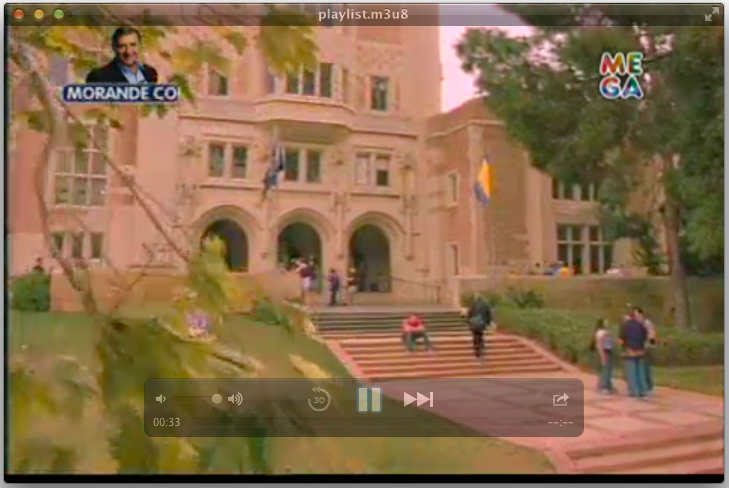
\includegraphics[scale=0.3]{imgs/qt-mega.png} & 
	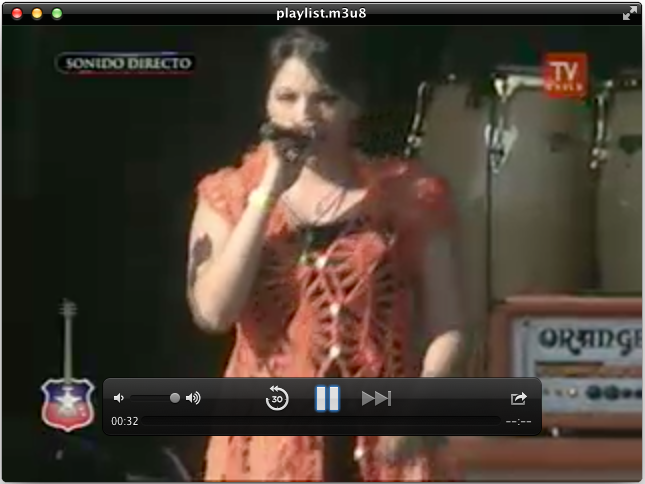
\includegraphics[scale=0.3]{imgs/qt-tvn.png} \\
	\end{tabular}
	\caption{Captura de Quicktime reproduciendo lista de reproducción a través de un URL.}
	\label{qt-tvn-mega}
\end{figure}

Utilizando \textbf{Wireshark} se observaron los datos entregados al cliente desde el servidor como \textit{\textbf{cookies}} indicadas en \ref{subsec:cookies}.

\begin{figure}[H]
	\centering
\begin{lstlisting}
HTTP/1.1 200 OK
Server: nginx/1.2.0
Date: Sat, 24 Nov 2012 18:06:10 GMT
Content-Type: application/vnd.apple.mpegurl
Transfer-Encoding: chunked
Connection: keep-alive
Keep-Alive: timeout=20
X-Powered-By: PHP/5.3.15-1~dotdeb.0
Set-Cookie: stream=tvn
Set-Cookie: t0=1353186024
Set-Cookie: tp=1353780370
Set-Cookie: ti=1353186033
Set-Cookie: tl=1353186085
Set-Cookie: si=1
Set-Cookie: sf=6

#EXTM3U
#EXT-X-TARGETDURATION:10
#EXT-X-PROGRAM-DATE-TIME:2012-11-17T18:00:33-03:00
#EXT-X-VERSION:3
#EXT-X-MEDIA-SEQUENCE:1
#EXTINF:13,
http://ssdemo.altavoz.net/streams/tvn/tvn_1353186033.ts
#EXTINF:10,
http://ssdemo.altavoz.net/streams/tvn/tvn_1353186043.ts
#EXTINF:9,
http://ssdemo.altavoz.net/streams/tvn/tvn_1353186052.ts
#EXTINF:12,
http://ssdemo.altavoz.net/streams/tvn/tvn_1353186063.ts
#EXTINF:7,
http://ssdemo.altavoz.net/streams/tvn/tvn_1353186070.ts
#EXTINF:13,
http://ssdemo.altavoz.net/streams/tvn/tvn_1353186085.ts
\end{lstlisting}
\caption{Información HTTP entregada por servidor Web}
\label{lst:setcookies}
\end{figure}

De la figura \ref{lst:setcookies} se puede observar que el servidor web Ngnix\cite{bib:ngnix-homepage} entrega en la cabecera HTTP las instrucciones Set-Cookie con los valores descritos en \ref{subsec:cookies}. \\

En la siguiente conexión con el servidor, se ajustaran los valores de las \textit{cookies} acorde al contenido de la lista de reproducción entregada. Como se describió anteriormente las \textit{cookies} no son manejadas por la aplicación cliente, ya que el sistema operativo iOS se encarga de manejar los valores de éstas.\\

En la figura \ref{lst:sequence2} se puede observar que los nuevos valores de cookies son establecidos por el servidor para la lista de reproducción acorde a la segunda secuencia del stream.

\begin{figure}[H]
	\centering
\begin{lstlisting}
HTTP/1.1 200 OK
Server: nginx/1.2.0
Date: Sat, 24 Nov 2012 18:06:25 GMT
Content-Type: application/vnd.apple.mpegurl
Transfer-Encoding: chunked
Connection: keep-alive
Keep-Alive: timeout=20
X-Powered-By: PHP/5.3.15-1~dotdeb.0
Set-Cookie: stream=tvn
Set-Cookie: tp=1353780385
Set-Cookie: ti=1353186043
Set-Cookie: tl=1353186093
Set-Cookie: si=2
Set-Cookie: sf=7

#EXTM3U
#EXT-X-TARGETDURATION:10
#EXT-X-PROGRAM-DATE-TIME:2012-11-17T18:00:43-03:00
#EXT-X-VERSION:3
#EXT-X-MEDIA-SEQUENCE:2
(...)
\end{lstlisting}
\caption{Información HTTP entregada por servidor Web con la lista actualizada para secuencia 2}
\label{lst:sequence2}
\end{figure}



%http://ssdemo.altavoz.net/playlist/playlist.m3u8?s=tvn&t=1353186024&c=0
%http://ssdemo.altavoz.net/playlist/playlist.m3u8?s=video1&t=1353186024&c=0

%escribir en consola el URL, probarlo en quicktime, vlc, navegador, app, wireshark para ver cookies

\section{Proceso corriendo en fondo} % background

Debido a que se utiliza el protocolo HTTP Live Streaming con el fin de entregar información en vivo, la instancia de AVPlayer se mantiene realizando peticiones por nuevas listas de reproducción a medida que pase el tiempo, sin importar que la reproducción se encuentre \textbf{pausada} o que la aplicación esté corriendo en el \textbf{fondo} (\textit{background}).\\

Se detectó un problema al interrumpir la reproducción. Fuera cualquiera el motivo, por ejemplo recibir una llamada telefónica, el sistema iOS envía la aplicación cliente a \textit{background} pausando la reproducción. Al volver después de la interrupción la aplicación retoma la reproducción, sin embargo el tiempo que ha pasado resulta en listas de reproducción distintas a la que se estaba viendo.\\

Se buscó la solución y se halló estableciendo una marca de tiempo de 30 segundos, acorde a la ventana de transmisión de la lista, asociada a la instrucción de pausa y reproducción del reproductor, que además es llamada por el botón \textit{Play/Pause} en la interfaz gráfica.\\

Al enviar la aplicación a background se guarda la \textbf{fecha del contenido} del stream y el momento en el cual se ha pausado.
Al volver a \textit{foreground} se activa el método para reanudar la reproducción donde se compara el momento de pausa guardado y el actual. Si esta diferencia es mayor a 30 segundos, se realiza una nueva llamada al servidor mediante URL. Sin embargo cuando la diferencia es menor, se reanuda la reproducción debido a que la fecha del contenido del stream aun se encuentra dentro del rango en la lista que posee la instancia de AVPlayer.\\

El valor de 30 segundos se debe una lista de reproducción con mínimo 3 segmentos de 10 segundos.\\

El problema encontrado se detectó por la depuración de la aplicación ejecutándose en un dispositivo iOS (iPhone). Se revisó el valor del \textbf{rango de reproducción} a través de notificaciones por cambios (página \pageref{item:seekableTimeRanges}). A pesar que la reproducción se pausaba o la aplicación se mandaba a background el rango se mantenía en aumento.

%escribir en consola los seekable time ranges, poner pausa background y al retomar reproducir, se notó que avanzaba la lista de iguañl forma. se arregó guardando la fecha al momento de poner pausa. que se llamaba al irse a background.

\section{Cambio de ancho de banda}

El cambio de ancho de banda se revisó mediante Wireshark y modificando el valor de la cadena de consulta \textbf{c} entre 0 (WiFi) y 1 (red celular) en el URL.\\ 

Por ejemplo: \url{http://ssdemo.altavoz.net/playlist/playlist.m3u8?s=tvn&t=1353186024&c=0}
La respuesta fue rastreada obteniendo una lista de reproducción:

\begin{figure}[H]
	\centering
\begin{lstlisting}
#EXTM3U
#EXT-X-STREAM-INF:PROGRAM-ID=1,BANDWIDTH=320000
stream.m3u8?s=tvn&t=1353186024
#EXT-X-STREAM-INF:PROGRAM-ID=1,BANDWIDTH=65000
stream.m3u8?s=tvn&a=1&t=1353186024
\end{lstlisting}
\caption{Lista de reproducción resultante de una petición al servidor con parámetro c = 0}
\label{lst:playlistc0}
\end{figure}

\begin{figure}[H]
	\centering
\begin{lstlisting}
#EXTM3U
#EXT-X-STREAM-INF:PROGRAM-ID=1,BANDWIDTH=65000
stream.m3u8?s=tvn&a=1&t=1353186024
#EXT-X-STREAM-INF:PROGRAM-ID=1,BANDWIDTH=320000
stream.m3u8?s=tvn&t=1353186024
\end{lstlisting}
\caption{Lista de reproducción resultante de una petición al servidor con parámetro c = 1}
\label{lst:playlistc1}
\end{figure}

En el caso de ajustar el valor a 1, la lista de reproducción invierte la prioridad de las variantes del stream, priorizando el enlace que posee sólo audio para un ancho de banda de \textbf{65 Kbps}. \ref{lst:playlistc1}

%se especifica requerimiento a la empresa, se modifica el dispatcher con lista de variantes, se revisa en wireshark.
%luego se utiliza la herramienta network link conditioner para modificar el BW en plena transmisión, revisar wireshark cuando cambia y ver en la misma app.
%Luego se prueba con iPhone cambiando entre wifi y 3g

  \subsection{WiFi: Wireless LAN}
  El comportamiento monitorizado a través del rastreo de paquetes se observa con el dispositivo real (iPhone) para comprobar la práctica de la teoría.
  En el caso de iniciar el stream en un iPhone con conexión a Internet mediante WiFi se presenta en pantalla el video inmediatamente si es que el ancho de banda da abasto. En caso que no sea suficiente cambiará a alguna variante capaz de reproducirse según el ancho de banda identificado por el dispositivo, en el ejemplo de la figura \ref{lst:playlistc0} la variante de menor tasa \textbf{65000 bps}, sólo audio.
  
  
  
%  se agrega campo en el URL para priorizar distintas variantes, con wifi video, 3g audio.
%  explicar que parte con el video, mostrar 2 imagenes emparejadas.

  \subsection{Red Celular: 3G o Edge}
%  con 3g, imagen de que muestra el audio primero.
En el caso de conexión a través de red celular el parámetro \textbf{c = 1} causa que el stream comience con la pista de audio inmediatamente, para luego evaluar si el ancho de banda es suficiente como para mostrar la variante con video.

\begin{figure}[H]
	\centering
	\begin{tabular}{cc}
	
\includegraphics[scale=0.2]{imgs/cell-link-1.png} & 
	
\includegraphics[scale=0.2]{imgs/cell-link-2.png} \\
	
\includegraphics[scale=0.2]{imgs/cell-link-3.png} & 
	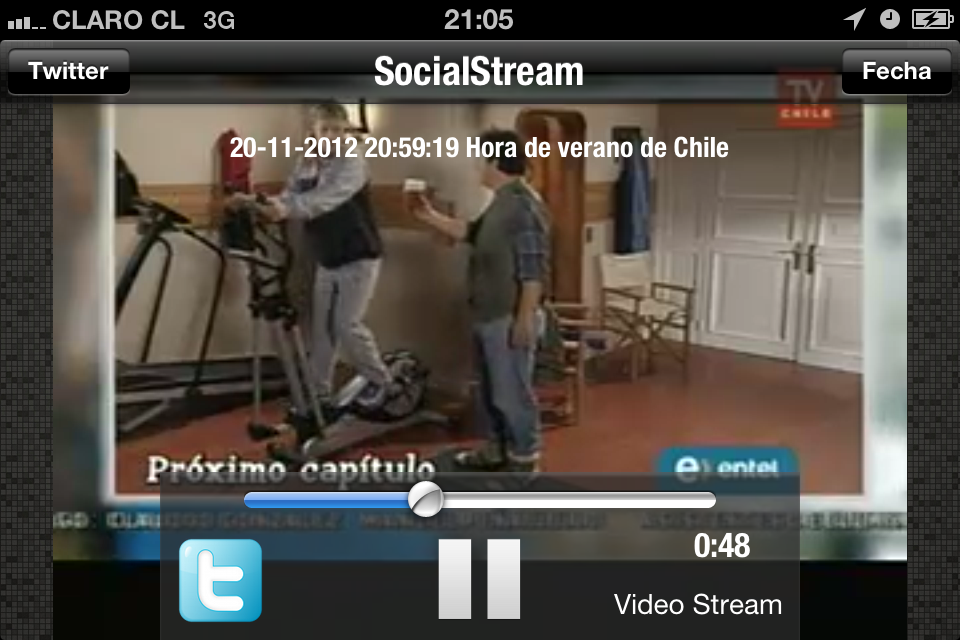
\includegraphics[scale=0.2]{imgs/cell-link-4.png} \\
	\end{tabular}
	\caption{iPhone reproduciendo stream de una fecha en particular a través de la red celular con enlace 3G.}
	\label{fig:cell-link}
\end{figure}

En la figura \ref{fig:cell-link} anterior se observa la secuencia de cambio de variante del stream. En la esquina inferior derecha del reproductor es posible observar el estado de las variantes, de izquierda a derecha pasa por los estados: Audio Stream, Cargando Video Stream, Video Stream. las imágenes 2 y 3 de la figura \ref{fig:cell-link} muestran el mismo estado a pesar que presentan distintas variantes, esto se debe a que para observar el estado de las variantes se  incorporó a la instancia de AVPlayer un observador del atributo \textit{tracks}, (página \pageref{item:kvo-tracks}, \textbf{Pistas de medios}) para comparar constantemente si alguna de las pistas son del tipo \textit{AVMediaTypeVideo}. 
En caso de observar cambios entre pistas que incluyen video a sólo pistas de audio y viceversa, se identifica el cambio de variante del stream.


\section{Cambio de transmisión mediante Twitter}
%- se revisa usando safari desktop con script que incluye player
%Gracias al modo desarrollador disponible en el navegador web para OS X Safari, es posible identificarse con el servidor utilizando un agente de usuario de Mobile Safari (iOS).

Para probar el cambio de stream a través de enlaces distribuidos por Twitter se alojó el script \textbf{PHP} (\ref{subsec:php-redir}) en un servidor dispuesto por AltaVoz S.A. La ubicación de éste corresponde a \url{http://tsh.altavoz.net/twitter/index.php}.
El script utiliza los argumentos en la cadena de consulta \textbf{s} y \textbf{t} para generar un URL compatible si corresponde, o en caso contrario mostrar un mensaje de incompatibilidad.

%  \subsection{Dentro de la aplicación}
  \subsection{Cambio de transmisión con la aplicación en ejecución}
  \label{subsec:ts-inside}
Se utiliza la llamada al método \textit{didSelectRowAtIndexPath:(NSIndexPath *)indexPath} gatillado al pulsar en un celda de la vista de tablas (fig. \ref{sshot-twitterclientvc}) utilizada para representar los Tweets asociados al \textit{hashtag} \textbf{\#SocialStream}. \\

\begin{figure}[H]
	\centering
	\begin{tabular}{cc}
	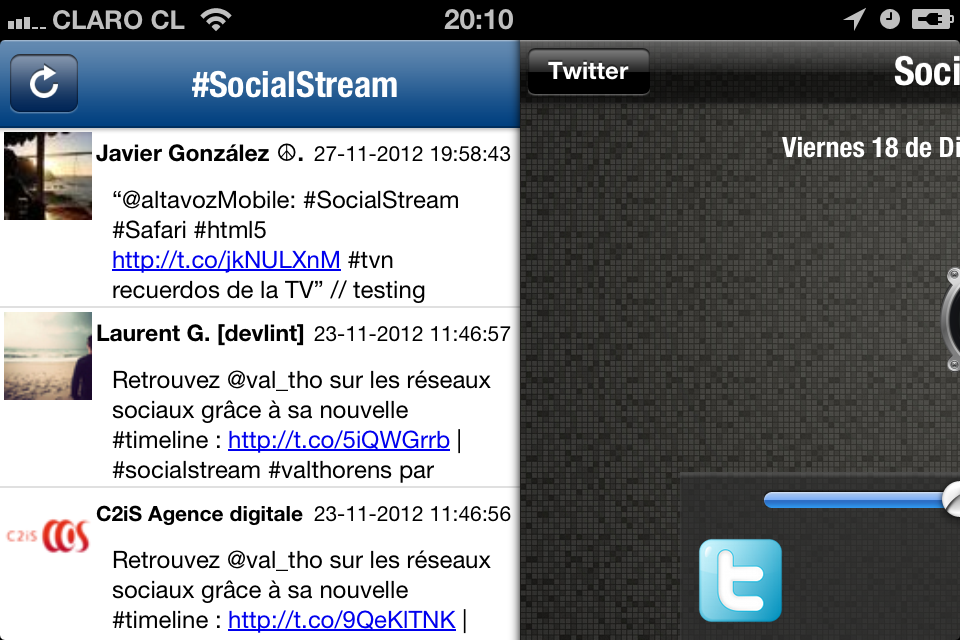
\includegraphics[scale=0.3]{imgs/twclient-list.png}
	\end{tabular}
	\caption{Vista de tabla con celdas compuestas de Tweets}
	\label{fig:twclient-list}
\end{figure}

El índice entregado al método se utiliza para identificar los datos del mensaje en el NSDictionary generado a partir del archivo JSON obtenido mediante Twitter Search API. De los datos contenidos en la instancia del diccionario \ref{tweet-json} se utiliza el valor de la clave \textbf{expanded\_url} para extraer la ruta del URL y generar un URL destinado al servicio \textbf{Bit.ly}.  \\

Del ejemplo en la figura \ref{fig:twclient-list} la primera celda presenta el dato \url{http://t.co/jkNULXnM}, el cual tiene como valor de \textbf{expanded\_url} asociado \url{http://bit.ly/Soxy8c}.

Esta ruta \textbf{Soxy8c}, que en realidad es el \textit{hash} bit.ly se utiliza para generar el URL:\\
\url{http://api.bit.ly/v3/expand?login=altavozchile&apikey=R_5947943f0ea1fe5b21df8269df2b4234&hash=Soxy8c}. \\

El resultado de esta llamada corresponde a un JSON que debe ser serializado a un NSDictionary y luego buscar en su clave \textbf{long\_url} los valores \textbf{s} y \textbf{t} de la cadena de consulta (fig. \ref{fig:twclient-debug}).\\

\begin{figure}[H]
	\centering
	\begin{tabular}{cc}
	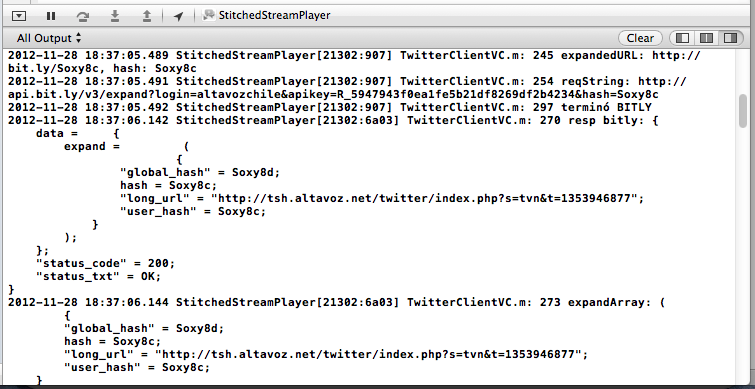
\includegraphics[scale=0.55]{imgs/twclient-debug.png}
	\end{tabular}
	\caption{Respuesta de bit.ly en la consola del depurador de Xcode.}
	\label{fig:twclient-debug}
\end{figure}


Si existen valores para \textbf{s} y \textbf{t} se procede a generar una notificación a la clase encargada de entregar el URL del stream a la instancia AVPlayer (fig. \ref{fig:twclient-results}, primera foto). En caso contrario se presenta al usuario un aviso con la clase \textbf{UIAlertView} indicando que el URL contenido en el mensaje no corresponde a un stream, dando la opción además de ser abierto en el navegador del sistema Mobile Safari mediante el método \textit{[[UIApplication sharedApplication] openURL:(NSURL*)url]}, logrando además que la aplicación se coloque en \textit{background} (fig. \ref{fig:twclient-results}, segunda foto).

\begin{figure}[H]
	\centering
	\begin{tabular}{cc}
	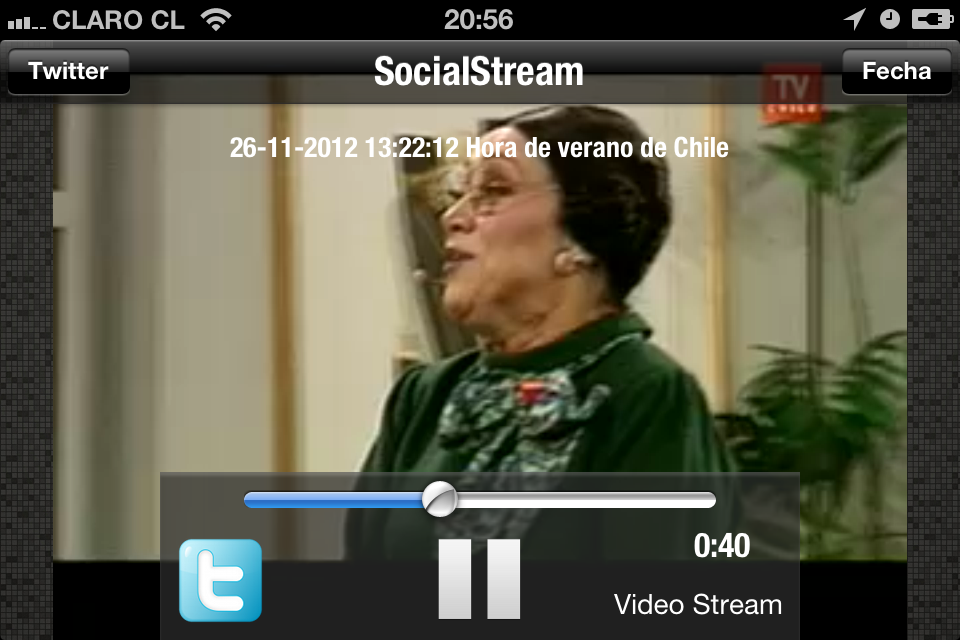
\includegraphics[scale=0.2]{imgs/twclient-stream.png} & 
	
\includegraphics[scale=0.2]{imgs/twclient-nostream.png} \\
	\end{tabular}
	\caption{Distintos resultados de apertura de URLs contenidos en mensaje de Twitter}
	\label{fig:twclient-results}
\end{figure}


%	- debug viendo el cambio de tranmisión, URL generado y definiendo el mismo canal. manejo en caso de tweet sin enlace
%	se genera notificación interna con los componentes. ver que cambia el stream.

%{
%    "display_url" = "bit.ly/Soxy8c";
%    "expanded_url" = "http://bit.ly/Soxy8c";
%    indices =     (
%        46,
%        66
%    );
%    url = "http://t.co/jkNULXnM";
%}
%
%http://api.bit.ly/v3/expand?login=altavozchile&apikey=R_5947943f0ea1fe5b21df8269df2b4234&hash=Soxy8c
%
%    data =     {
%        expand =         (
%                        {
%                "global_hash" = Soxy8d;
%                hash = Soxy8c;
%                "long_url" = "http://tsh.altavoz.net/twitter/index.php?s=tvn&t=1353946877";
%                "user_hash" = Soxy8c;
%            }
%        );
%    };
%    "status_code" = 200;
%    "status_txt" = OK;
%}
%  \subsection{Scheme registrado en iOS}
  \subsection{Cambio de transmisión con el scheme registrado en iOS}
  
  Para revisar el comportamiento de la aplicación al ser lanzada por el sistema debido a la apertura de un URL que presenta el \textit{scheme} registrado, es necesario configurar el \textbf{Depurador} (\textit{debugger}) del entorno de desarrollo Xcode (anexo \ref{anexo:xcode-debug}) de forma que se encuentre a la espera de la apertura de la aplicación (fig. \ref{fig:xcode-waitforapp}), esto es diferente al comportamiento usual donde cada vez que se ejecuta en el compilador se lanza automáticamente en el dispositivo.\\

  \begin{figure}[H]
	\centering
	\begin{tabular}{cc}
	
\includegraphics[scale=0.7]{imgs/xcode-waitforapp.png}
	\end{tabular}
	\caption{Entorno de desarrollo Xcode en modo de espera de apertura de la Aplicación.}
	\label{fig:xcode-waitforapp}
\end{figure}

%Con esta configuración de depuración, ya es posible 
Con el depurador configurado en modo espera (anexo \ref{anexo:xcode-debug}) es posible revisar el comportamiento con enlaces abiertos desde otra aplicación de iOS, como por ejemplo desde la aplicación de terceros Tweetbot. En la figura \ref{fig:tweetbot-sstream} al pulsar en el URL del tweet, el script desarrollado para la redirección (\ref{subsec:php-redir}) identifica el \textbf{Agente de Usuario} de la clase UIWebView presuntamente utilizada por Tweetbot para redirigir a un URL con el \textit{scheme} asociado por la aplicación cliente. El resultado se muestra en la segunda imagen donde el procedimiento consiste en generar una notificación a la clase que contiene la instancia de \textbf{AVPlayer} de forma que genere el URL necesario para reproducir el stream.\\

Al ser iniciada por esta vía, la aplicación gatilla el método de la clase delegada como instancia principal de la aplicación (\textit{AppDelegate}):\\

\textit{- (BOOL)application:(UIApplication*)application handleOpenURL:(NSURL*)url}\\

Dentro de esta llamada se generan las notificaciones encargadas de entregar un URL correspondiente al stream del instante compartido. Realizando pruebas se descubrió que la entrega de los datos a la aplicación no generaban el comportamiento esperado, es decir la visualización del stream en el preciso instante, esto debido a que el método encargado de manejar el URL se ejecutaba con anterioridad a los métodos de iniciación del reproductor, por lo tanto para asegurar la entrega de la información se programó un observador por notificación \cite{bib:ios-nsnotificationcenter} atento al aviso de carga del controlador de vistas que contiene la instancia del \textbf{AVPlayer} encargado de reproducir. \\

El aviso se realiza desde el método \textit{- (void)viewDidAppear:(BOOL)animated} del controlador de vistas, así es posible saber que las vistas, incluyendo la del reproductor, se han cargado en pantalla y proceder a entregar el URL del contenido.



\begin{figure}[H]
	\centering
	\begin{tabular}{cc}
	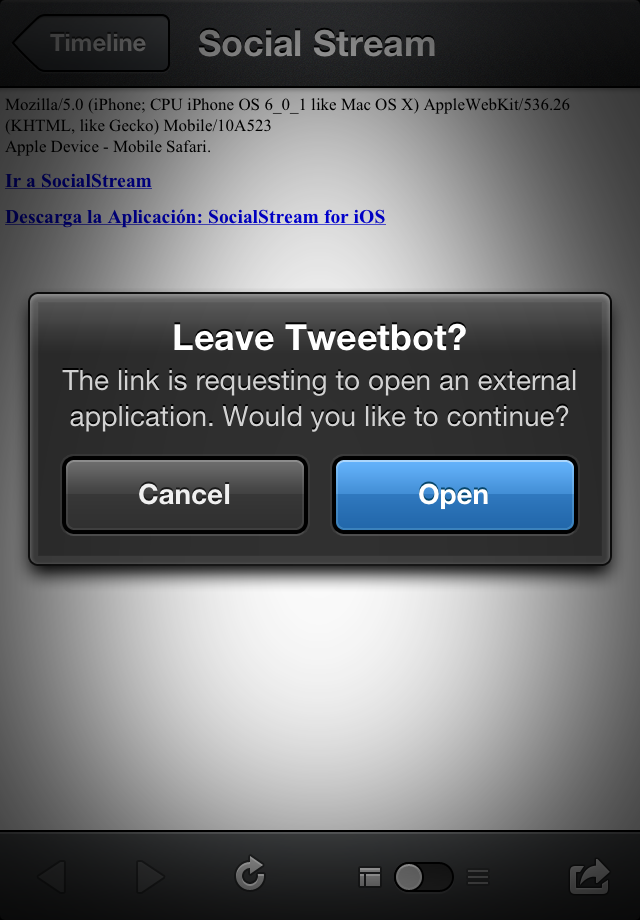
\includegraphics[scale=0.3]{imgs/tweetbot-sstream.png} &
	
\includegraphics[scale=0.3]{imgs/tweetbot-appopened.png} \\
	\end{tabular}
	\caption{Solicitud de Tweetbot para abrir una aplicación externa y su posterior resultado.}
	\label{fig:tweetbot-sstream}
\end{figure}

\section{Enlaces Twitter en otros dispositivos}
A continuación se presentan los resultados de la apertura de URL compartidos a través de la aplicación cliente a través de distintas plataformas.
%	pantallazos de páginas de error, el por qué y cómo se entregan según el script, no se revisa internet explorer porque se utilizaron navegadores compatibles con OS X.
	
  \subsection{PC Escritorio}
  Se presentan capturas de pantalla de la reacción del script desarrollado con distintos navegadores web compatibles con Mac OS X. Ese es el motivo por cual Internet Explorer no aparece en estos resultados, ya que desde su versión 5.2.3 lanzada el 16 de junio de 2003 \cite{bib:mac-iexplorer} no existe soporte para sistema operativo nombrado.

    \subsubsection{Safari}
El navegador web Safari al ser producto de las tecnologías desarrolladas por Apple es compatible para la reproducción de streams HLS. Para mostrar el contenido se utilizó la marca de HTML5  \textless VIDEO\textgreater \ con la lista de reproducción generada por el script php como fuente de video. El resultado es el reproductor visto en la figura \ref{fig:uagent-safari}.\\

Además también en pruebas se utilizó el widget dispuesto por Twitter \cite{bib:twitter-widget} para embeber tweets relacionados a cierto hashtag, en este caso: \#SocialStream. El uso de este widget solo fue por motivos de experimentación.
%      safari muestra un player html5
%    foto del player

  \begin{figure}[H]
	\centering
	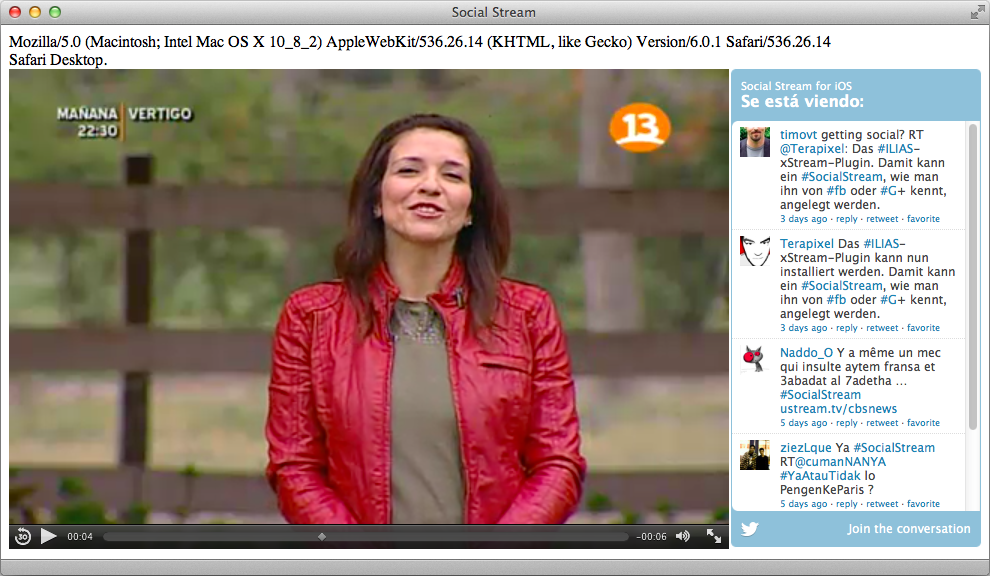
\includegraphics[scale=0.4]{imgs/uagent-safari.png} 
	\caption{Apertura de enlace compartido desde la aplicación cliente en Safari.}
	\label{fig:uagent-safari}
\end{figure}  
    
    \subsubsection{Chrome}
  \begin{figure}[H]
	\centering
	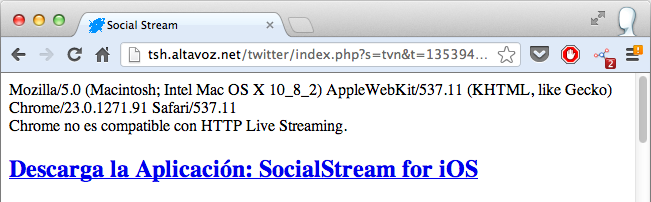
\includegraphics[scale=0.6]{imgs/uagent-chrome.png} 
	\caption{Apertura de enlace compartido desde la aplicación cliente en Google Chrome.}
	\label{fig:uagent-chrome}
\end{figure}  
    \subsubsection{Firefox}
  \begin{figure}[H]
	\centering
	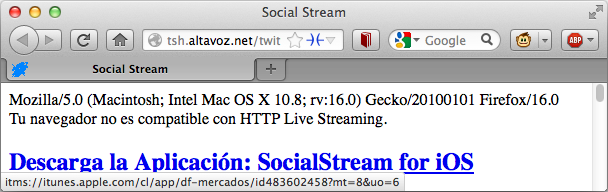
\includegraphics[scale=0.6]{imgs/uagent-firefox.png} 
	\caption{Apertura de enlace compartido desde la aplicación cliente en Mozilla Firefox.}
	\label{fig:uagent-firefox}
\end{figure}  
    \subsubsection{Opera}
  \begin{figure}[H]
	\centering
	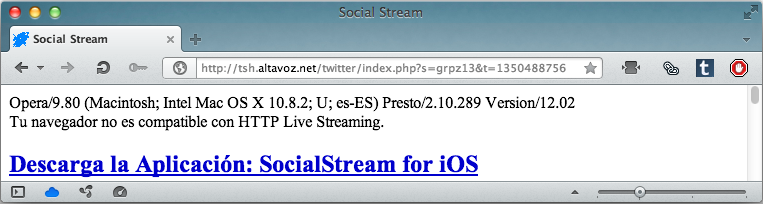
\includegraphics[scale=0.55]{imgs/uagent-opera.png} 
	\caption{Apertura de enlace compartido desde la aplicación cliente en Opera.}
	\label{fig:uagent-opera}
\end{figure}  
  \subsection{Android y otros móviles incompatibles}
  En el caso del celulares con el sistema operativo Android se presenta el mensaje de la figura \ref{fig:uagent-android}. Si bien desde la versión 4.0, Android OS es compatible con HTTP Live Streaming, es necesario desarrollar una aplicación similar a la hecha para iOS.
 \begin{figure}[H]
	\centering
	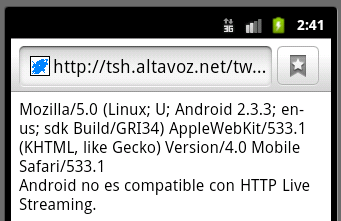
\includegraphics[scale=0.7]{imgs/uagent-android.png} 
	\caption{Apertura de enlace compartido desde la aplicación cliente en Safari.}
	\label{fig:uagent-android}
 \end{figure}  

%  pantallazo del cell de la esperanza
%  explicar que tampoco es compatible con HLS, por lo menos 2.3, 4.0 ICS en adelante es compatible, pero para reproducir el stream se debe desarrollar una aplicación cliente similar a la hecha en iOS

\section{Comparación con SocialStream Flash}

En las figuras \ref{sshot_iOS_sstream} y \ref{fig:eag-player} se puede observar el reproductor del stream de video distribuido a través del protocolo RTMP. El reproductor fue desarrollado por un alumno de la Universidad Técnica Federico Santa María para demostrar la capacidad de cambiar el tiempo del contenido en un reproductor de video desarrollado con las tecnologías de Adobe Flash.

\begin{figure}[H]
	\centering
	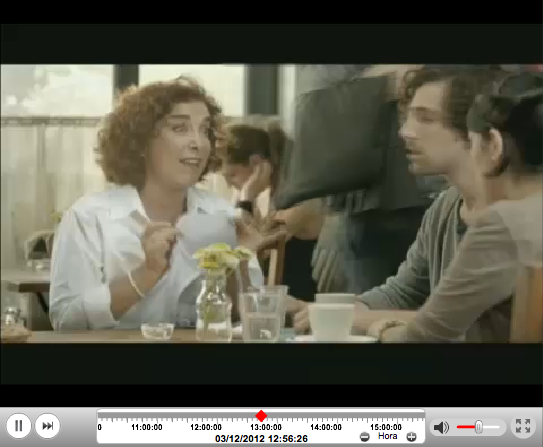
\includegraphics[scale=0.6]{imgs/eag-player.png} 
	\caption{Reproductor Flash para Timeshift en Navegador web Safari.}
	\label{fig:eag-player}
\end{figure}  

En las figuras \ref{fig:twclient-results} y \ref{fig:cell-link} se presenta el reproductor desarrollado por el autor de este documento como resultado del proyecto del tema de memoria.\\

En esta sección se destacan las diferencias de usabilidad de los reproductores para el usuario final, más allá de la gran diferencia que el reproductor de la figura \ref{fig:eag-player} y el desarrollado en iOS se utilizan en plataformas distintas. 

\begin{itemize}
\item \textbf{Protocolo:} El reproductor Flash utiliza protocolo RTMP mientras que el reproductor para iOS recibe el contenido a través de HTTP Live Streaming.
\item \textbf{Salto de Tiempo:} la forma de saltar en el tiempo en el reproductor flash precisa de clicks con mouse, ya sea para cambiar la escala de su linea de tiempo como para moverse el punto central de reproducción, lo cual dificulta en gran medida el consumo del contenido mientras se busca otro instante.\\

En el caso del reproductor iOS se utiliza el control explicado en la sección \ref{subsec:datepicker}, que permite elegir un tiempo en especifico pulsando el botón \textbf{Cargar} o cancelar la selección de fecha pulsando fuera del área del selector sin intervenir el contenido en reproducción.

\item \textbf{Entrega de contenido:} El contenido en el reproductor Flash presenta una mayor exactitud al elegir un tiempo en especifico, esto debido a que la segmentación del video es cada 5 segundos. En el caso de HTTP Live Streaming es recomendado por los ingenieros de Apple que desarrollaron el protocolo, utilizar 10 segundos como mínimo para cada segmento de video o audio. El motivo de esta recomendación es evitar paralizaciones (\textit{stalls}) en la transmisión a través de redes celulares \cite{bib:tensec-targetduration}.\\

\item \textbf{Redes Sociales:} Ésta fue una característica adicional a la solución de permitir transmisión con saltos en el tiempo en iOS. Durante el desarrollo de la aplicación cliente se descubrió el potencial de realizar cambios de lista de reproducción del protocolo HTTP Live Streaming a través de cadenas de consulta de los URLs y compartir el contenido a través de redes. En el caso del reproductor Flash el cambio temporal se realiza a través de la comunicación bidireccional del protocolo RTMP mediante la función \textit{seek} enviada desde el cliente (especificación RTMP \cite{bib:rtmp-specs} sección 4.2.7 - \textit{seek}).
\end{itemize}
%mostrar player original de eduardo, la diferencia de la linea de tiempo, el salto de tiempo, la exactitud y que no es tan exacto porque los segmentos son de 10 segundos

%la linea de tiempo difiere con una representación gráfica, se utilizó el control de fecha para simplificar el punto a elegir, además la linea de tiempo precisa de mouse over para mostrar datos y en el caso táctil difiere mucho.




	%Incluir capítulo Conclusiones
	
\chapter{Conclusiones y trabajo futuro}
%# pagina y media no mas de 2

%explicar que apenas se terminó, el proyecto se usó como base para janus cooperativa, pero solo radio.
%es posible generar productos en base al reproductor, se puede mejorar la interfaz gráfica con preparativos en base a diseño de interfaces junto a especialistas como diseñadores gráficos.
%además el trabajo sienta base para la compartición de contenido en vivo a través de plataformas móviles, muy similar a la tendencia actual de las llamadas smart tv que tambien incorporan redes sociales.

%# contenido
\section{Conclusiones}

El trabajo de memoria significó en grán medida la investigación de las tecnologias de Apple Inc. En un principio se tuvo como fin lograr compatibilizar el contenido distribuido con tecnologías de Adobe Inc. (RTMP) en iOS. 
Sin embargo se descubrió las grandes trabas que Apple pone para su entorno aplicaciones, instando y casi obligando a utilizar sus tecnologias. 
Por lo tanto se tuvo que presentar estos motivos y convencer a la empresa interesada en este proyecto de adoptar un nuevo sistema de distribución para los dispositivos iOS con HTTP Live Streaming. Teniendo claro este punto se tuvo que idear la forma de igualar la caracteristica de saltar el tiempo en la tranmisión. \\ 

Llegando a utilizar la cadena de consultas en el URL que el cliente utiliza para pedir los contenidos al servidor se dio paso al desarrollo de una aplicación cliente que permite al usuario manejar el punto de reproducción. Esto significó la investigación del lenguaje de programación \textbf{Objective-C} y el Kit de desarrollo de iOS. En materia de diseño se siguieron los patrones sugeridos por Apple para sus aplicaciones, buscando simpleza para el usuario en seleccionar un punto en especifico.\\

Además se debe tomar en cuenta que las sugerencias para el protocolo HTTP Live Streaming se indican con el fin de entregar la mejor experiencia en lo que respecta el consumo de la tranmisión. Materia que tuvo que se conversada con la empresa interesada debido a reluctancias por parte de esta en seguir al pie de la letra ciertas sugerencias, como por ejemplo la duración de cada segmento, sólo por el hecho de haber utilizado otro valor con el sistema desarrollado para RTMP.\\

El desarrollo para el alumno significó adoptar nuevos lenguajes de programación que no fueron una dificultad gracias a la formación en la universidad con lenguajes de programación similares. El desarrollo con PHP y Objective-C fueron fundamentales para incorporar las caracteristicas claves de este proyecto.\\

Si bien pudo haber existido otros caminos para el fin conseguido de este proyecto, se diseñó una solución con una arquitectura tal que permitiera integrarla a otras plataformas que compatibilizen con el protocolo HTTP Live Streaming, como ya ha sido adoptado por el sistema operativo Android (desde 4.0). \\


%Existen muchas alternativas y caminos para crear una solucion a un problema de administracion como el que se planteo en este trabajo, pero el gran desafio, fuera de completar el desarrollo de esta, era encontrar una manera de que la arquitectura de la solucion permitiera una modularidad tal, que fuera fácil la integración de nuevas herramientas y tecnologías.\\

%	el trabajo precisó de investigación a fondo de las tecnologias de Apple Inc. adentrarse en el sistema iOS y su riguroso cuidado para las apps, estudiar las tecnologias en desarrollo por parte de ellos, leer los drafts en desarrollo de http live streaming, lo necesario para especificar el dispatcher que es algo fuera de lo normal para el protocolo.
%	el estudio del SDK, las clases de stanford, guidelines.

%# claves	
%	usar http live streaming.
%	por qué tuve que insistir en apegarse a las recomendaciones de apple siendo que se preferian otras en altavoz.
%	compatibilidad desde ios 5.0 en adelante	solo por pto flotante en lista de segmentos.

%# malas
%	mala decision fue investigar portar rtmp, para darse cuenta que no sería permitido por apple, utilizar segmentos de 5 segundos, ventanas de tranmisión muy angostas y también muy amplias. el no 
	
		
	% lo mas importante del trabajo 
	% las decisiones claves y el por que de estas
	% decisiones malas tambien
	
%60 paginas MAX HASTA CONCLUSIONES

	\section{Trabajo Futuro}
%	mostrar timeline nueva, desarrollo en la empresa.
%	preview en popup
%	redes sociales facebook
%	destacados del editor
%	inclusión de favoritos
%	boton rtune
La version del cliente desarrollado para este trabajo de memoria cumple con los requisitos iniciales de permitir saltos en el tiempo en la transmisión que provee el servidor encargado del dispatcher. Sin embargo el gran potencial de las aplicaciones en iOS permiten expandir la experiencia de usuario aun más. En un trabajo futuro se puede mejorar el cliente con:
\begin{itemize}
\item Diseñar e implementar un modelo de datos que entregue momentos destacados de la transmisión desde el servidor, controlado por el gestor de los contenidos para generar más audiencia en momentos precisos.

\item Implementar sistema de Analisis de comportamiento de usuario del tipo Google Analytics, el cual está disponible para iOS. Análogo a un \textit{people-meter} de la televisión actual.

\item Integrar más redes sociales aparte de Twitter, como \textbf{Facebook} o \textbf{Sina Weibo} que han sido integradas al Social Framework de \textbf{iOS 6} debido a su gran popularidad.

\item Permitir al usuario guardar momentos como favoritos de forma privada y localmente en su dispositivo sin necesidad de compartir el punto de reproducción. Para esto es necesario desarrollar un modelo de datos locales para la aplicación.

\item Integrar comportamientos originales. Por ejemplo saltar entre momentos de la transmisión con solo un botón, similar a la función \textbf{Re-Tune} de los televisores que permiten saltar entre dos canales. Una nueva variante temporal expandiría aun más la experiencia del usuario.
\end{itemize}

	
	%EXTENSIONES PARA hacerle, que no las haré pero mejorarian el producto en si, facebook, otras redes, etc
	% todo list

	
	%Para armar Indice que quiere el profe
	%archivo_indice.tex
\chapter{Anexos}
	\section{Sistemas operativos}
	El desarrollo del proyecto de memoria tuvo como fin un aplicación para el sistema operativo iOS. Para esto fue necesario utilizar las herramientas dispuestas por Apple Inc.
		\subsection{OSX}
La décima versión del sistema operativo para computadores Macintosh, la X se refiere al numero romano 10. Esta versión posee un micronúcleo Mach, junto a servicios de sistema operativo de tipo UNIX basados en FreeBSD.
Las aplicaciones para OSX se desarrollan utilizando \textbf{Cocoa} API, la interfaz de programación de aplicaciones orientada a objetos.
\subsubsection{Xcode}
Para este proyecto se utilizó el entorno de desarrollo \textbf{Xcode}, el cual está solamente disponible para OSX.\\

Xcode se puede obtener desde la tienda de aplicaciones de OSX, el repositorio que integra el mismo sistema de pago utilizado en la tienda de música digital iTunes Store (fig. \ref{fig:xcode-appstore}).
\begin{figure}[H]
	\centering
	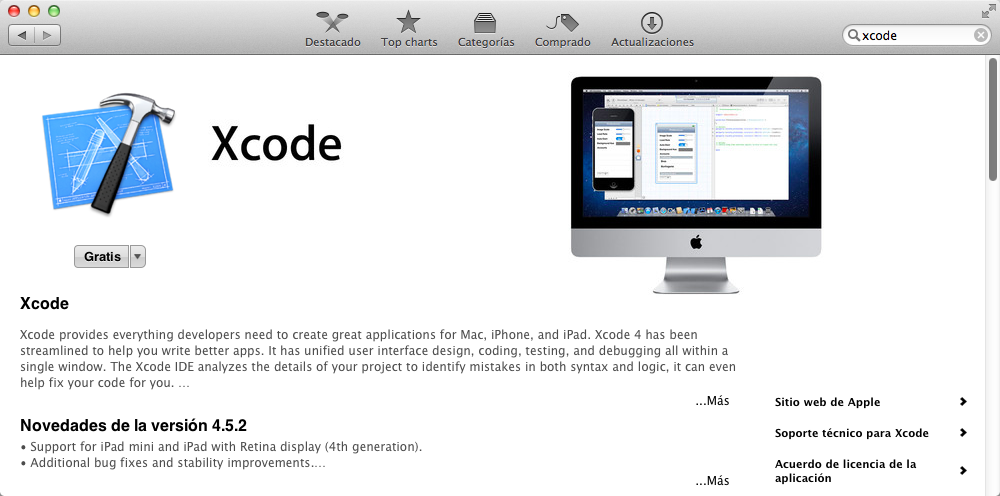
\includegraphics[scale=0.41]{imgs/xcode-appstore.png} 
	\caption{Xcode disponible gratis en la \textbf{App Store}, la tienda de aplicaciones para OSX}
	\label{fig:xcode-appstore}
\end{figure}  
%		os x, se empezó el desarrollo en lion, migración de xcode 3 a 4, inestabilidad
%		explicar como se usa  itunes con ios
		\subsection{iOS}
Sistema operativo para dispositivos móviles, originalmente fue desarrollado para iPhone, sin embargo se ha utilizado en nuevos productos de Apple como iPod Touch, iPad, y el Apple TV. Su caracteristica principal es la interfaz de usuario basada en manipulación de gestos táctiles por parte del usuario, es decir pellizcos, deslizamientos o toques con los dedos.\\

iOS deriva de Mac OSX en su arquitectura de diseño, utilizando también el mismo micronucleo Mach basado en FreeBSD: Darwin.\\

El desarrollo de sus aplicaciones se realiza con \textbf{Cocoa Touch} API (fig. \ref{fig:ios-cocoatouch}).
\begin{figure}[H]
	\centering
	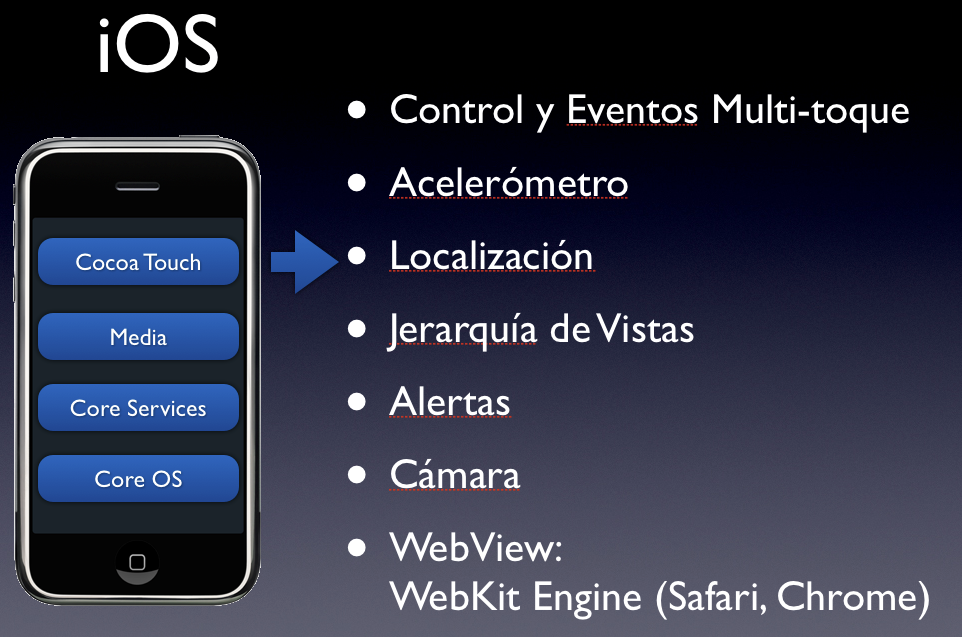
\includegraphics[scale=0.35]{imgs/ios-cocoatouch.png} 
	\caption{Caracteristicas de la API Cocoa Touch.}
	\label{fig:ios-cocoatouch}
\end{figure}  



%		se empezó con ios 4, pasamos a 5, luego 6		
%		facilidad de actualizacion

	\section{Hardware}
		Se presentan los implementos necesarios para desarrollar el proyecto de memoria.
		\subsection{Macintosh}
	%http://en.wikipedia.org/wiki/Unified_Extensible_Firmware_Interface
	
%The use of EFI as opposed to the traditional BIOS. The BIOS found in most PCs is designed for backwards-compatibility to allow the use of older software and operating systems. As Mac OS X has nothing that tied it to the BIOS, it was free to use an alternative firmware that eliminates some of the shortcomings of the BIOS. EFI is not exclusive to Macs, however; motherboards can be purchased off-the-shelf that support EFI, and some computer retailers use it as well now.
%Non-standard motherboard form factors. The motherboards in all current Macintosh models do not correspond to a form factor found in other retailer's computers, such as ATX or ITX.
%Unique case deigns. Macintosh cases are designed to be slightly more "classy" looking than those found with the standard "white box" PC.
%Incompatible expansion cards. Because of the aforementioned use of EFI, off-the-shelf expansion cards such as graphics cards cannot be used in a Mac. Similar models designed for use with EFI can be purchased from the Apple store, at a typically higher markup price. This,too, will probably change as EFI becomes more widespread.

		\subsection{iPhone, iPad, iPod Touch}
		descripcion de iphone, cuando salió, presentación de steve, revolucion del smartphone, pasar de teclas a nuevas pantallas táctiles.
		ipad, nueva forma de leer, reemplaza netbook, 3g pero no llama, creó un nuevo mercado y es lider
		ipod, comezó como música, luego de iphone adopta ios, explicar que es alternativa a iphone, gran adopcion en usa.  lider en players.
	\section{Frameworks}
	uikit, descripción 
	avfoundation, descripcion
	mpmedia framework, descripcion
	%entorno de desarrollo utilizado
	
%\chapter{Bibliografia}
	% refencias de lo estudiado y utilizado para el trabajo	
		
	%Incluir capítulo 4
	%	\chapter{Diseño de un protocolo con topología de árbol}

Debido a los resultados obtenidos en la evaluación energética de la implementación del protocolo PEGASIS descrita en el capítulo 3, se decidió diseñar e implementar un nuevo enfoque de recolección de datos, utilizando una técnica que permita reducir el consumo del TMoteSky en los tiempos de idle listening. Se optó por implementar un árbol de ruteo, similar a la construcción de red propuesta en el estándar IEEE 802.15.4, construido para utilizar la herramienta Low Power Listening para reducir el consumo de corriente del dispositivo. \\

\section{Visión general del diseño}

El diseño comienza con la búsqueda de una estrategia de ahorro energético que permita reducir el consumo de corriente del TMoteSky, atacando el problema del consumo de corriente del chip CC2420 en estado idle. Posteriormente, se diseña el '' Componente de recolección'', un esquema de formación y control de la topología, que permite establecer una red con topología de árbol multihop y mantener la recolección de datos incluso si se presentan nodos muertos. 

\section{Estrategias de ahorro energético}
El perfil del consumo de corriente del TMoteSky, está dominado principalmente por el consumo del transceptor CC2420.

\begin{table}[H]
  \centering
  \caption{Principal consumo de corriente en el TMoteSky  \cite{TelosBConsumo}}
 \includegraphics[scale=0.5]{imgs/ConsumoTmoteSky.eps}
\end{table}

Como se muestra en el cuadro 4.1, el consumo del CC2420 representa más del 90\% del consumo total del dispositivo.\\

Para los dispositivos que soportan TinyOS, se han planteado dos estrategias de ahorro energético: La primera consiste en utilizar un ciclo de trabajo sincronizado, donde los dispositivos mantienen sus radios apagadas por periodos largos de tiempo y las enciendan por periodos cortos, realizando este ciclo de manera sincronizada en toda la red; o, utilizar la técnica ''Low Power Listening'', que consiste en apagar la radio y encenderla periódicamente, por periodos de tiempo cortos, para sensar el canal y detectar cuando otro dispositivo quiere transmitir un mensaje.\\

La primera estrategia requiere un protocolo de sincronización de tiempo, que consiste en un conjunto de operaciones y mensajes que se intercambian en la red para mantener secciones o la totalidad de la red sincronizada en el tiempo. TinyOS provee un protocolo llamado ''Flooding Time Sync Protocol'' (Protocolo de sincronización de tiempo por inundación, FTSP), que consiste en inundar la red con el tiempo del nodo con menor TOS\_NODE\_ID en la red (''tiempo global''). Sin embargo, se ha documentado que la implementación para la radio CC2420 hereda un bug de la implementación de la interfaz PacketTimeStamp para el CC2420\cite{FtspBug}. El error causa que continuamente los receptores del mensaje de sincronización obtengan un tiempo global errado por decenas de milisegundos, lo que eventualmente causa la pérdida de sincronización.\\

La estrategia ''Low Power Listening'' tiene el objetivo de disminuir el consumo de corriente, disminuyendo el tiempo de idle listening y a su vez permite que la red sea asincrónica. Para lograr estos objetivos, la implementación toma las medidas siguientes:

\begin{itemize}
\item Se implementa un ciclo de poder para la radio (ciclo LPL), es decir, ciclo de radio encendida y radio apagada.
\item La radio se mantiene encendida el tiempo suficiente para detectar un carrier en el canal.
\item Si detecta un carrier, se mantiene encendida la radio para recibir el mensaje.
\item Cuando se envía un mensaje, se extiende el tiempo de duración del preámbulo hasta el tiempo de duración del ciclo LPL.
\end{itemize}

\begin{center}
\begin{figure}[H]
\centering
\includegraphics[scale=0.625]{imgs/GraficoTiemposLPLsoloLPL.eps} 
\caption{Gráfico del consumo de corriente que tiene el TmoteSky con módulo LPL activado, cuando realiza operaciones escucha en bajo consumo.}
\end{figure}
\end{center}

\begin{center}
\begin{figure}[H]
\centering
\includegraphics[scale=0.625]{imgs/GraficoTiemposLPLTX.eps} 
\caption{Gráfico del consumo de corriente que tiene el TmoteSky con módulo LPL activado, cuando transmite un paquete con extensión de preámbulo.}
\end{figure}
\end{center}

 Debido a la ausencia de un protocolo robusto de sincronización de tiempo implementado para TinyOS y a que implementar un protocolo de esta naturaleza está fuera del alcance de este trabajo, se decidió utilizar la estrategia ''Low Power Listening'' para gestionar el consumo de corriente del TMoteSky. En el  Anexo C, se describe en detalle la utilización de este componente y se realiza una caracterización del consumo para distintos escenarios.

\section{Diseño del componente de recolección}

Al igual que la implementación del protocolo PEGASIS, se construye el protocolo de red sobre la pila de comunicación ''Radio Stack'' que provee TinyOS. Además, se decide incluir otras mejoras no exploradas antes: Una cola de reenvío, para reducir las posibilidades de perder mensajes; y mensajes de datos con carga de largo variable, para dar libertad a la aplicación usuaria del protocolo a que utilice una estructura de datos arbitraria para sus datos. Siguiendo el mismo esquema de implementación que CTP y Dissemination, el protocolo debe implementar las funciones Send y Receive, que proveerán las funciones de red necesarias para que el nodo pueda enviar y recibir mensajes al Gateway.
%Diagrama del Stack
%\begin{center}
%\begin{figure}[H]
 %\centering
 %\includegraphics[scale=0.4]{imgs/Stack.eps}
 %\caption{Stack}
%\end{figure}
%\end{center}
\subsection{Formato de mensajes}
En las próximas secciones se mencionarán de forma recurrente los mensajes definidos para esta implementación, por lo que a continuación se describen los dos tipos de mensajes diseñados para el protocolo árbol: Mensajes de Topología y Mensajes de Datos Multihop.\\ 

Los mensajes de topología son todos los mensajes intercambiados para la formación y mantención de la topología de árbol de la red, a los cuales se les asigna el AM Type 0x20.
%Topology Message
\begin{table}[H]
  \centering
  \caption{Descripción de la estructura de un mensaje de topología.}
 \includegraphics[scale=0.5]{imgs/MensajesProtocoloMultihopTopologia.eps}
\end{table}

Dentro de los mensajes de topología establecen los siguientes tipos: ''beacon request'', ''beacon response'', ''join request'', ''join response ok'' y ''join response denied''.

%Multihop Message Header
\begin{table}[H]
  \centering
  \caption{Descripción de la estructura de un mensaje de datos.}
 \includegraphics[scale=0.5]{imgs/MensajesProtocoloMultihopMensajeDato.eps}
\end{table}

Los mensajes de datos multi-hop son los que transportan los datos generados por la aplicación a través de la red, a los cuales se les asigna el AM Type 0x21. Para estos mensajes sólo se define la cabecera, ya que el resto del mensaje variará según como sea definido por la aplicación.

%Secuencias
\subsection{Descripción de secuencias y lógica}
En esta sección se describen las secuencias de mensajes y la lógica que se implementa para la formación de una red con topología de árbol. Para formar el árbol de asociación se utiliza el esquema planteado por la IEEE 802.15.4 \cite{IEEE802154}, 
%Secuencia de Asociación
\subsubsection{Secuencia de Asociación}
Para formar el árbol de recolección se utiliza un sistema de beacons (faros). Los nodos descubren la red enviando un mensaje de ''Beacon Request'', que sólo será respondido por un nodo que ya se encuentre en la red. El Gateway asume el rol de raíz y primer beacon, y en consecuencia, a partir del descubrimiento del Gateway, la red se ramifica en forma de árbol. La secuencia de asociación que propone este esquema consiste en el intercambio de cuatro mensajes:\\
 
 \textbf{BEACON\textunderscore REQUEST:} Este mensaje es utilizado para permitir que el nodo emisor encuentre la red. Debe incluir al menos la dirección origen, para permitir que los nodos que estén en la red le respondan con un mensaje BEACON\textunderscore RESPONSE, y debe ser direccionado a la dirección de broadcast.\\
 
 \textbf{BEACON\textunderscore RESPONSE:} Este mensaje se envía en respuesta a un BEACON\textunderscore REQUEST. Sólo puede ser enviado por un nodo que ya esté asociado a la red y debe proveer la información necesaria para que el nodo que está ingresando a la red pueda decidir entre varios mensajes BEACON\textunderscore RESPONSE el que estime como el mejor candidato para negociar una asociación.\\
 
 \textbf{JOIN\textunderscore REQUEST:} Si el nodo que está tratando de asociarse a la red ha recibido mensajes BEACON\textunderscore RESPONSE y ha determinado un nodo candidato para realizar la negociación de asociación, envía un mensaje de JOIN\textunderscore REQUEST dirigido al nodo candidato. Este mensaje debe contener al menos la dirección de origen del nodo que realiza este requerimiento.\\
 
 \textbf{JOIN\textunderscore RESPONSE:} Un nodo que está en la red que recibe un JOIN\textunderscore REQUEST debe responder al nodo que ha solicitado la asociación con la red en forma positiva o negativa. Este mensaje debe contener al menos la dirección origen y la respuesta a la asociación.\\
 
 %Diagrama de secuencia de asociación
\begin{figure}[H]
 \centering
 \includegraphics[scale=0.45]{imgs/DiagramaSecuenciaAsociacion.eps}
 \caption{Diagrama UML de secuencia de asociación}
\end{figure}

En la figura 4.3 se muestra la secuencia que se desea implementar para asociar un nodo que entra a la red (Nodo A) con otro que ya está en la red (Nodo B). Primero, nodo A envía un mensaje broadcast BEACON\textunderscore REQUEST, el nodo B escucha el mensaje y envía un BEACON\textunderscore RESPONSE. El nodo A espera un tiempo arbitrario, denominado "BEACON\_REQUEST\_INTERVAL" , que permite que el nodo A reciba y almacene temporalmente varios mensajes BEACON\textunderscore RESPONSE. Si el nodo ha recibido mensajes beacon request y ha determinado un candidato para solicitar la asociación a la red, envía un JOIN\textunderscore REQUEST al candidato. Si no ha encontrado ningún candidato, vuelve a enviar un BEACON\textunderscore REQUEST.

%Secuencia de Multihop
\subsubsection{Secuencia de envío y reenvío de mensajes multihop}
En esta secuencia se intercambian dos tipos de mensajes.\\

\textbf{MH\textunderscore DATA:} Estos mensajes pueden ser generados por un nodo que está asociado a la red y son los que transportan datos entregados por la capa de aplicación. Estos mensajes deben ser capaces de ser generados con largo variable, para permitir a la aplicación que envíe dentro de estos mensajes las estructuras de datos que estime convenientes. La cabecera debe ser de un largo definido y debe al menos incluir: la dirección de origen del mensaje, un número de secuencia y el largo del mensaje. La dupla formada por la dirección del mensaje y número de secuencia funciona como una ''clave primaria'' que permite identificar, de forma única, un mensaje. La identificación de un mensaje es útil para tolerar fallas y la organización de los mensajes en el destino final, por ejemplo, una base datos. Estos mensajes pueden ser generados por un nodo, o bien, recibidos por un nodo para posteriormente ser reenviados.\\

\textbf{ACK:} Este tipo de mensaje debe ser generado cada vez que un nodo recibe un mensaje MH\textunderscore DATA para informar al nodo fuente del mensaje, que el nodo intermedio o destino ha recibido el mensaje correctamente. Estos mensajes son de sólo un salto, ya que como este protocolo es diseñado para realizar el "mejor esfuerzo" no se implementan ACKs multihop.\\

%Diagrama de secuencia multihop
\begin{figure}[H]
 \centering
 \includegraphics[scale=0.45]{imgs/DiagramaSecuenciaMultihop.eps}
 \caption{Diagrama de secuencia de asociación}
\end{figure}

En la figura 4.4 se observa la secuencia de envío de un mensaje Multihop. El nodo A determina que su próximo salto es el nodo B y envía un mensaje MH\textunderscore DATA al nodo B. El nodo B responde con un ACK si recibe el mensaje correctamente, sino no envía mensaje alguno.  Luego el nodo B determina que el próxima salto es el nodo C y reenvía el mensaje recibido hacia el nodo C. Está secuencia debe continuar a través de todos los nodos intermedios hasta que finalmente llega al Gateway.

%Secuencia de Reconexión
\subsubsection{Secuencia de reconexión}
Puede suceder que un nodo presente algún tipo de falla, agote su batería o simplemente desaparezca aparentemente de la red. En ese caso, los nodos que rutean mensaje a través de él, deben detectar que este nodo ya no está presente. Ya que los nodos cuando reciben un mensaje de datos deben confirmar con un ACK, un nodo puede identificar que un nodo ha desaparecido aparentemente por la pérdida de ACKs.\\

%Diagrama de Reconexión
\begin{figure}[H]
 \centering
 \includegraphics[scale=0.45]{imgs/DiagramaSecuenciaReconexion.eps}
 \caption{Diagrama de secuencia de renovación de la asociación}
\end{figure}

La secuencia de desconexión y reconexión comienza con la pérdida sucesiva de ACKs, digamos que el nodo A está ruteando mensajes a través del nodo B, y el nodo B aparentemente desaparece. Cuando el nodo A intenta enviar un mensaje MH\textunderscore DATA al nodo B,éste no responde con un ACK, por lo tanto el nodo A puede identificar un ACK perdido. Luego de un número definido arbitrariamente de ACKs perdidos, el nodo A deja la asociación con el nodo B. Posteriormente, el nodo A vuelve a buscar un padre utilizando la secuencia de asociación descrita anteriormente.

%Secuencia BROADCAST
\subsubsection{Secuencia de MHData Broadcast}
 Es posible, que la aplicación requiera enviar un mensaje de datos para configurar la aplicación de uno, varios o todos los nodos. Al no utilizar direcciones, ni tablas de ruteo que indiquen el camino a un nodo en particular, no se puede generar una ruta específica a un nodo X desde el Gateway. Otros protocolos similares de recolección (ver CTP más Dissemination) realizan esta funcionalidad mediante una inundación o diseminación del mensaje, a través de toda la red. Para emular este comportamiento, se decide diseñar una funcionalidad de "broadcast de red" para los mensajes de datos, que pueda ser utilizada por cualquier nodo de la red. El esquema que se propone es el siguiente:

\begin{itemize}
\item Se agrega al mensaje MH\textunderscore DATA los campos: bcast\textunderscore seqnum, para que un nodo pueda diferenciar los mensajes de broadcast; y bcast\textunderscore radio, para establecer cuál es el radio (en términos de reenvío) de alcance del broadcast.

\item Cuando un nodo se prepara para enviar un mensaje de broadcast, debe especificar que este mensaje es de broadcast, asignar un valor de  bcast\textunderscore seqnum coherente y un radio de alcance.

\item El nodo que recibe un mensaje de broadcast debe utilizar el bcast\textunderscore seqnum para decidir si es necesario reenviar o no el mensaje.

\item Una vez que ha decidido reenviar el mensaje, debe decrementar el valor del bcast\textunderscore radio para indicar a los próximos saltos que el mensaje ya ha avanzado un nodo en el radio de alcance.
\end{itemize}

\subsubsection{Encolamiento y reenvío de mensajes}
Para reducir la pérdida de mensajes, se diseña una cola de mensajes que permita encolar los mensajes generados por el nodo y los mensajes recibidos desde otros nodos que deben ser reenviados. Una cola FIFO permite un ordenamiento intrínseco de los mensajes, donde el primer mensaje ingresado estará asociado a la cabeza de la cola FIFO (head) y el último estará en la cola (tail).\\ 	
%Diagrama de encolamiento de mensajes
%\begin{figure}[H]
 %\centering
 %\includegraphics[scale=0.625]{imgs/DiagramaColaFifo.eps}
% \caption{Diagrama de encolamiento de mensajes}
%\end{figure}

Las secuencias, funcionalidades y componentes descritos se implementarán en forma de una Configuración NesC, de forma similar a como se realiza con PEGASIS en el capítulo 3. En el próximo capítulo se describirá como se implementa este diseño para TinyOS, utilizando LPL para realizar las operaciones en ultra bajo consumo. Además se revisan las pruebas de verificación para cada componente y funcionalidad, junto con la evaluación energética correspondiente.
	
	%Incluir capítulo 5
	%	\chapter{Implementación del protocolo con topología de árbol}

\section{Descripción de la implementación}
La implementación del esquema de recolección propuesto en la sección anterior, se realiza programando un ''Componente de recolección'', se divide en dos módulos:  el ''Componente de ruteo'', que es el encargado de formar la red y establecer la ruta hacia el punto de recolección; y la implementación del componente de reenvío, que es el encargado de encolar y reenviar los mensajes.\\

\subsection{Componente de Recolección - CollectionC}
La implementación del componente de recolección, diseñado en capítulo 3, comienza con la programación de una configuración nesC que provee una interfaz similar a la que provee CTP\cite{TEP123}. La configuración se denomina CollectionC, y provee la implementación de las interfaces: \textbf{SplitControl, Send, Receive y Broadcast}. La descripción  de CollectionC se realiza en el archivo CollectionC.nc.

\begin{figure}[H]
	\centering
 	\includegraphics[scale=0.5]{imgs/DiagramaComponenteCollectionC.eps} 
 	\caption{Diagrama de componentes de la configuración CollectionC}
\end{figure}

En la figura 5.1 se describe la configuración utilizando el lenguaje visual de descripción de componentes y sus relaciones, propuesto en el libro TinyOS Programming\cite{TinyOSProgramming}. La configuración consta de dos grandes módulos: El \textbf{módulo RouterP y el módulo ForwardeP}. El módulo RouterP se encarga de incorporar el nodo a la red, proveer al módulo ForwarderP del próximo salto, y tolerar fallas debido a la desaparición de nodos de la red. El módulo ForwarderP se encarga de: colocar en la cola de envío los mensajes que la aplicación necesita enviar (interfaz Send); recibir los mensajes de los nodos hijos; encolar los mensajes recibidos; y detectar la desaparición de nodos. \\

Para que el usuario pueda configurar los parámetros de funcionamiento del protocolo se provee el archivo Config.h, donde, mediante definiciones para el preprocesador C, el usuario puede configurar parámetros que se describirán en esta sección.

\subsection{Componente RouterP}
%Qué es?
El componente Router es el que implementa las secuencias de asociación y reconexión. El componente provee a la configuración la interfaz SplitControl y al módulo ForwarderP la interfaz RouterInfo.

%Interfaz SplitControl-Secuencia de Asociación Beacon Request
\subsubsection{Interfaz SplitControl}
La implementación comienza con la programación de la interfaz SplitControl. Esta interfaz permite a la capa de aplicación, iniciar el componente de ruteo utilizando el comando SplitControl.start(). Cuando se invoca este comando, este inicia el componente LPL con el intervalo definido como LPL\textunderscore INTERVAL en el archivo Config.h. A continuación, inicia la pila ActiveMessage y el timer BeaconRequestTimer con el intervalo BEACON\textunderscore REQUEST\textunderscore INTERVAL, configurable en Config.h. De esta forma se inicia la secuencia de asociación y durante este periodo se mantiene el estado del nodo en la red como NO\textunderscore NWK (sin red). \\

Durante el tiempo que transcurre entre cada BEACON\textunderscore REQUEST, el nodo almacena los BEACON\textunderscore RESPONSE, y cuando se gatilla nuevamente el timer, determina el mejor candidato para realizar la asociación. Si el nodo ha recibido mensajes BEACON\textunderscore RESPONSE y ha determinado un candidato para solicitar la asociación a la red, envía un JOIN\textunderscore REQUEST al candidato. Si no ha encontrado ningún candidato, vuelve a enviar un BEACON\textunderscore REQUEST.\\

Se implementan dos formas de determinar el candidato para requerir asociación: Por mayor RSSI, elige el nodo ''más cercano electromagnéticamente''; y por menor profundidad, se elige el nodo de menor profundidad en la red, pero que tenga un RSSI mayor a -87[dBm], que se ha medido como el mínimo para garantizar una tasa de recepción de mensajes correctos de 85\%  \cite{RSSIUnder}. La utilización de uno de estos esquema se deja configurable en el archivo Config.h, mediante las definiciones SELECT\_BEACON\_BY\_RSSI y SELECT\_BEACON\_BY\_DEPTH. \\

Cuando el nodo recibe un mensaje JOIN\textunderscore OK el nodo establece sus variables de red depth (profundidad) y parent (padre), con los valores obtenidos de este mensaje. Posteriormente cambia al estado IN\_NWK, activando el envío de ACKs con la interfaz CC2420Config y señalizando el evento SplitControl.startDone(SUCCESS) a la aplicación. La señalización de este evento permite que la aplicación esté en conocimiento del momento en que dispone de red para poder enviar mensajes de datos al Gateway.\\

Un punto importante en la implementación, es la incorporación de un sistema de ''Despliegue forzado de la red'', similar al desarrollado para la implementación de PEGASIS, para permitir el desarrollo de pruebas multihop en el laboratorio. El sistema utiliza la matriz ''hopsMatrix'', que implementada en un arreglo bidimensional que describe con un 0, 1 ó 10 la posibilidad de comunicación entre dos nodos. 

\begin{figure}[H]
	\centering
 	\includegraphics[scale=0.5]{imgs/hopsmatrix.eps} 
 	\caption{Ejemplo de matriz utilizada para el sistema de despliegue forzado }
\end{figure}

En la figura 5.2. se muestra una de las matrices utilizada para las pruebas. Cero se utiliza sólo para representar la relación entre un nodo con sí mismo; un 1 en una fila M y columna N, indica que el nodo M puede recibir mensajes del nodo N; mientras que un 10 en la fila M y columna N, indica que el nodo M no puede recibir mensajes del nodo N. Por ejemplo: el 1 en la posición (0,1) indica que el nodo 0 puede recibir mensajes del nodo 1; mientras que el 10 en la posición (0,2), indica que el nodo 0 no puede recibir mensajes del nodo 2. Cuando está activado el despliegue forzado, se utiliza la función ''bool isVisible(uint16\_t id)'' para revisar si un mensaje recibido se procesará o no. Para activar el despliegue forzado, basta con definir ''FORCED\_DEPLOYMENT'' en el archivo Config.h.

\subsection{Componente ForwarderP}
El componente ForwarderP es el encargado de implementar las secuencias de envío y reenvío multihop. Provee a la configuración las interfaces Init, Send, Receive y ForwarderInfo. ForwarderInfo es la interfaz desarrollada para proveer información desde el Forwarder a otros componentes.
%Interfaz Init?

\subsubsection{Interfaz Send}
La implementación del componente Forwarder comienza con la implementación de la interfaz Send. La interfaz Send proporciona el comando Send.getPayload, el comando Send.send, y el evento Send.sendDone.\\

El comando Send.getPayload se utiliza para proporcionar a la aplicación el espacio de memoria para que escriba el mensaje datos que desea enviar. Este comando recibe como entrada un puntero a una estructura ''message\textunderscore t''  y el tamaño del mensaje. Con estos datos, el comando se encarga de crear el espacio de memoria para el mensaje, del tamaño solicitado por la aplicación más el tamaño de la cabecera  ''MHData'', según lo definido en la sección 4.3.1. Finalmente, retorna un puntero a la dirección del payload del mensaje. Esta implementación, permite a la aplicación la utilización de mensajes de largo variable y no limitar a la aplicación a utilizar mensajes de un largo fijo.\\

El comando Send.send es el que permite a la aplicación colocar un mensaje en la cola de envío. Recibe como entrada un puntero a la estructura del mensaje ''message\textunderscore t'' y el largo. 

\begin{figure}[H]
	\centering
 	\includegraphics[scale=0.6]{imgs/DiagramaFlujoComandoSendSend.eps} 
 	\caption{Diagrama de flujo de la implementación del comando Send.send}
\end{figure}

Como muestra el diagrama de flujo en la figura 5.3, el comando Send.send comienza llenando la cabecera del mensaje, utilizando la interfaz RouterInfo para obtener el padre del nodo y la profundidad a la cuál se encuentra en la red. Además, escribe en la cabecera  el campo originaddr con el TOS\textunderscore NODE \textunderscore ID del nodo, y el contador de mensajes de datos en el campo seqnum. Posteriormente, se utiliza la interfaz MessagePool para obtener un espacio de memoria para el mensaje utilizando el comando MessagePool.get(), y si la ejecución del comando resulta exitosa, se copia el mensaje desde la aplicación a la MessagePool. A continuación, se encola el puntero al mensaje almacenado en la MessagePool en la cola FIFO SendQueue, y si resulta exitoso, se encola la tarea sendTask.\\

\begin{figure}[H]
	\centering
 	\includegraphics[scale=0.6]{imgs/DiagramaFlujoSendTask.eps} 
 	\caption{Diagrama de flujo de la implementación de la tarea SendTask}
\end{figure}

%Hablar de la sendTask
La tarea sendTask, es una tarea nesC que se encarga de sacar los mensajes de la cola y enviarlos por el aire. Cada vez que se encola un mensaje, se realiza un post de la tarea sendTask. Si la cola no está vacía, la tarea extrae la cabeza de la cola (el mensaje encolado más antiguo) e intenta enviarlo por el aire, utilizando la pila ActiveMessage. Si el envío se realiza con éxito, el sistema invoca al manejador del evento sendDone (ver figura 5.5), si se ha recibido un ACK del nodo destinatario, el manejador del evento elimina el mensaje más antiguo en la cola y si la cola aún no está vacía, vuelve a realizar un post de la sendTask. Si no se ha recibido un ACK, se vuelve a realizar un post de la sendTask, pero sin eliminar el mensaje más antiguo de la cola, forzando su reintento.

\begin{figure}[H]
	\centering
 	\includegraphics[scale=0.6]{imgs/DiagramaFlujoMHSendDone.eps} 
 	\caption{Diagrama de flujo de la implementación del evento MHSend.sendDone}
\end{figure}

%Reenvío y enconlado de mensajes recibidos
\subsubsection{Interfaz MHReceive.receive}
El componente ForwarderP es el que implementa la interfaz MHReceive.receive, que es la que maneja el evento gatillado por la recepción de mensajes de datos multihop. 

\begin{figure}[H]
	\centering
	\includegraphics[scale=0.6]{imgs/DiagramaFlujoReceiveBroadcast.eps}
	\caption{Diagrama de flujo de la implementación del evento MHReceive.receive}
\end{figure}

Como se muestra en la figura 5.6, cuando se recibe un mensaje de datos, primero se revisa el campo ''type'' en la cabecera para revisar si es un mensaje broadcast. Si lo es, se revisan los campos ''originaddr'' y ''bcast\_seqnum'' para revisar si es un mensaje repetido, si no lo es, se actualiza la cabecera y se señaliza el evento Broadcast.Receive entregando a la aplicación el mensaje, el payload y el largo. Luego de que se señaliza el Broadcast recibido, el mensaje se vuelve a encolar (sólo si el bcast\_radius es mayor que 0 después de ser decrementado). Si el mensaje no era de tipo broadcast, entonces se encola en la cola FIFO SendQueue y se realiza un post de la tarea sendTask.
	
\subsubsection{Interfaz Broadcast}
La interfaz Broadcast se ha implementado con el objetivo de proveer al sistema un medio de comunicación hacia los nodos, que permita por ejemplo: configurar la frecuencia con la que realizan las mediciones, o el sensor del cuál se desean obtener mediciones. También se permite que un nodo envíe un broadcast a los nodos de la red. \\

Los procesos realizados para enviar un mensaje de broadcast son los mismos que se describen en la figura 5.4, de la implementación del comando Send. Difieren en que al llenar la cabecera, el campo ''type'' indica que es un mensaje de broadcast, el ''bcast\_seqnum'' se llena con un valor válido (se incrementa con cada envío broadcast) y también se llena el campo ''bcast\_radius'', con el radio que ha indicado la aplicación. Los procesos de reenvío de los mensajes de broadcast se describieron en la sección anterior.

\section{Pruebas de verificación}
%Prueba de esta funcionalidad
Las pruebas de verificación de la funcionalidades implementadas, se realizan utilizando el sistema de despliegue forzado y la aplicación WSNSniffer. Esta última se modificó para que soportara el formato de los nuevos mensajes especificados en la sección 4.3.1.
 
\subsection{Pruebas al módulo RouterP}
En esta sección se describen las pruebas realizadas y los resultados para verificar las siguientes funcionalidades del módulo RouterP: Descubrimiento de red, Secuencia de Asociación, Asociación por RSSI, Asociación por Profundidad.

\subsubsection{Descubrimiento de red}
La primera prueba consiste en verificar que el mensaje beacon request se envíe periódicamente mientras el nodo no encuentre un nodo en la red con el cuál asociarse. Para esta prueba se utiliza la aplicación de prueba SampleApp, que se encuentra en el CD adjunto a este trabajo, que periódicamente realiza una medición con el sensor de luz y la envía hacia el Gateway utilizando el protocolo implementado. Para esta prueba el TMoteSky que corre SampleApp tiene un ID igual a 1 y un intervalo BEACON\textunderscore REQUEST\textunderscore INTERVAL igual a 1[s].

\begin{table}[H]
\centering
\caption{Extracto del reporte del sniffer para la prueba de descubrimiento de red}
 \includegraphics[scale=0.5]{imgs/ResultadosProcesadosBeaconLoop.eps}
\end{table}

En el cuadro 5.1 se muestra el resultado de la prueba registrado por el sistema Sniffer. La columna ''Timestamp'' muestra el tiempo en que la aplicación Sniffer recibió el mensaje. En promedio, el tiempo de recepción del mensajes es de 975[ms], lo cuál está un 2,5\% por debajo del valor configurado. La columna ''Src Addr'' muestra el TOS\textunderscore NODE\textunderscore ID del dispositivo origen del mensaje, este corresponde al valor 1, que fue el valor configurado para el dispositivo utilizado para esta prueba. La columna ''Dest Addr'' muestra el TOS\textunderscore NODE\textunderscore ID del destinatario del mensaje, en este caso, corresponde a la dirección de broadcast 65535 o 0xFFFF en notación hexadecimal. Ambos identificadores son obtenidos de la cabecera Active Message, para diferenciarlos de los identificadores que se incluyen en la cabecera de los mensajes implementados para la red. La columna ''AM Type'' muestra el identificador Active Message que se ha definido para este tipo de mensajes, que corresponde a 32 (0x21 en hexadecimal) para los mensajes de Topología.\\

Se puede apreciar que tal como se describe la secuencia de asociación en el capítulo 3, el nodo envía beacon request periódicamente , aproximadamente cada 1[s] y se mantiene así al no existir una red en el radio de alcance. 

\subsubsection{Secuencia de Asociación}
A continuación se realiza la misma prueba, pero agregando el nodo Gateway, que por si solo se encuentra en la red, y que debería responder los beacon request del nodo de prueba.

\begin{table}[H]
\centering
\caption{Resultado de prueba de la secuencia de asociación}
 \includegraphics[scale=0.6]{imgs/ResultadosProcesadosTestsJoinRequest.eps}
\end{table}

%Comentario del resultado de la prueba
En el cuadro 5.2 se muestra el resultado registrado por el sistema sniffer para la prueba de secuencia de asociación satisfactoria. En el cuadro se observa que el dispositivo con TOS\textunderscore NODE\textunderscore ID 1 envía un mensaje con subtype = 0x0, que corresponde al mensaje de topología BEACON\textunderscore REQUEST\textunderscore , a la dirección de broadcast. El dispositivo de TOS\textunderscore NODE\textunderscore ID 0 (nodo Gateway) responde con tres mensajes con subtype igual a 0x1, que corresponde al mensaje de topología BEACON\_RESPONSE. El largo de la ráfaga de mensajes de respuesta es configurable en definición del  BEACON\textunderscore RESPONSE\textunderscore BLAST\textunderscore SIZE en el archivo Config.h, esto permite al nodo 1 obtener varias muestras de RSSI y obtener un promedio de estos valores, que le permitirán decidir cuál nodo elegirá como candidato de padre en la red. En cada uno de los mensajes BEACON\_RESPONSE, el campo destaddr igual a 0x0 indica que el nodo 0 está respondiendo al nodo 1. El campo depth igual a 0 indica que la profundidad del nodo 0 en la red es 0. El campo joining igual a 0x1 indica que el nodo está incorporando nodos hijos a la red. El campo isCollector igual a 0x1 indica que el nodo 0 es el recolector (y Gateway). A continuación, el nodo 1 responde al BEACON con un mensaje de subtype igual a 0x2, que corresponde al mensaje de topología JOIN\textunderscore REQUEST. El campo destaddr igual a 0x0 indica que el mensaje está dirigido al nodo 0, ya que el nodo eligió al nodo 0 como candidato de padre en la red. El campo  joining igual a 0x1, esto indicaría que el nodo 1 está aceptando asociaciones, pero ya que no está en la red, no responderá a mensajes BEACON\textunderscore REQUEST\textunderscore , ni el nodo 0 utilizará esa información en el proceso de asociación. El campo isCollector es igual a 0x0, indicando que el nodo 1 no es recolector. El campo redundancy es un campo que se utilizó de manera experimental y se mantuvo en la estructura del mensaje para futuros desarrollos.\\

\subsubsection{Verificación de asociación por mayor RSSI}
Para verificar la funcionalidad de asociación mediante la utilización del mayor RSSI, se realiza el siguiente experimento. Primero se despliegan espacialmente 3 nodos: nodo Gateway (0), nodo 1 y nodo 2. como se muestra en la figura 5.7

\begin{figure}[H]
	\centering
 	\includegraphics[scale=0.6]{imgs/TopologiaDesplieguePruebaAsociacionRssi.eps} 
 	\caption{Topología forzada para prueba de limitación de hijos}
\end{figure}

Como muestra la figura 5.7, los nodos se despliegan linealmente, donde el nodo 1 se encuentra a 3 [m] del nodo 0, mientras que el nodo 2 a 3.5[m] del nodo 0 y 0.5 del nodo 1. Con esta disposición, el nodo 2 debería medir diferencias entre los indicadores RSSI medidos para los mensajes del nodo 1 y el nodo 0.  El objetivo, es que el nodo 2 reciba beacons de ambos nodos, pero que elija el nodo que envió beacons con un RSSI promedio más alto. 

\begin{center}
\begin{table}[H]
\caption{Resultado de prueba de asociación por mayor RSSI}
 \includegraphics[scale=0.6]{imgs/ResultadosProcesadosTestsAsociacionRSSI.eps}
\end{table}
\end{center}

En el cuadro 5.3 se muestra la secuencia de mensajes capturada por el sniffer para la prueba. La secuencia capturada es la secuencia de asociación del nodo 2. Se observa que el nodo 2 en el tiempo 0:46:56:126 inicia la asociación enviando un BEACON\textunderscore REQUEST a la dirección de broadcast. Los nodos 0 y 1 responden con los respectivos mensajes BEACON\textunderscore RESPONSE. Luego, el nodo 2 elige unirse al nodo 1 y en el tiempo 00:46:57:083 envía un mensaje de JOIN\textunderscore REQUEST. Finalmente, recibe un JOIN\textunderscore OK para confirmar la asociación. El resultado de esta secuencia es la asociación del nodo 2 al nodo 1, que es lo esperado si es que el nodo 2 midió un RSSI promedio más alto de los mensajes BEACON\textunderscore RESPONSE del nodo 1 que del nodo 2. Sin embargo, con el sniffer no se puede confirmar ese comportamiento. Por esta razón, se implementó que el nodo 2 enviara por comunicación serial la tabla ' beaconList ', que es el arreglo bidimensional que utiliza para almacenar los datos de los BEACON\textunderscore RESPONSE recibidos.\\

\begin{center}
\begin{table}[H]
\caption{Output recibido por puerto serial del nodo 2}
 \includegraphics[scale=0.6]{imgs/OutputAsociacionRssi.eps}
\end{table}
\end{center}

En el cuadro 5.4 se muestran las 15 entradas, de las cuales sólo las primeras seis son válidas (campo valid igual a 65534 es válido y 65535 es inválido). Estas entradas válidas corresponden a seis mensajes BEACON\textunderscore RESPONSE que recibió el nodo 2. Las entradas 0, 1 y 2 corresponden a mensajes del nodo 0 y el promedio entero de sus RSSI es -32 [dBm]. Las entradas 3, 4 y 5 corresponden a mensajes del nodo 1 y el promedio entero de sus RSSI es 8 [dBm]. De esta manera, se verifica que el nodo 2 eligió como candidato para la asociación al nodo del que recibió los mensajes BEACON\textunderscore RESPONSE con mayor RSSI.\\

\subsubsection{Verificación de asociación por menor profundidad}
%Probar formas de asociación, DEPTH
Para verificar la funcionalidad de la asociación por menor profundidad, se utiliza el mismo despliegue no forzado utilizado y mostrado en la figura 5.7. Además, se vuelve a utilizar la herramienta ''printf'' para enviar por comunicación serial al computador la tabla 'beaconList'.

\begin{center}
\begin{table}[H]
\caption{Resultado de prueba de asociación por menor profundidad}
 \includegraphics[scale=0.6]{imgs/ResultadosProcesadosTestsAsociacionPorDepth.eps}
\end{table}
\end{center}

La secuencia de asociación comienza en el tiempo 0:38:56:207, cuando el nodo 2 envía un mensaje BEACON\textunderscore REQUEST a la dirección de broadcast. A continuación, los nodos 0 y 1 responden con los mensajes BEACON\textunderscore RESPONSE correspondientes. Luego, en el tiempo 0:38:57:164 el nodo 2 solicita una asociación al nodo 0, y este confirma la asociación en el tiempo 0:38:57:200. La secuencia resultante es la esperada de acuerdo al criterio de asociación por menor profundidad, debido a que el nodo 2 decide solicitar la asociación al nodo 0 en vez del nodo 1, ya que el nodo 0 tiene la menor profundidad. Sin embargo, para asegurar que el nodo no está siguiendo el criterio de RSSI, se revisa la tabla de beacons enviada por comunicación serial por el nodo al computador.

\begin{center}
\begin{table}[H]
\caption{Output recibido por puerto serial del nodo 2}
 \includegraphics[scale=0.6]{imgs/OutputAsociacionProfundidad.eps}
\end{table}
\end{center}

Como se observa en el cuadro 5.6, el nodo 1 tiene RSSI mucho mayores que el nodo 0, por lo que claramente el nodo 2 no utilizó el criterio de mayor RSSI para elegir el nodo al cual solicitar la asociación.

\subsection{Pruebas al módulo ForwarderP}
En esta sección se describen las pruebas realizadas y los resultados para verificar las siguientes funcionalidades del módulo ForwarderP: Verificación de reenvío de mensajes y Verificación de broadcast de red.

\subsubsection{Verificación de reenvío de mensajes}
Para verificar que el reenvío de los mensajes va de padre en padre hasta el Gateway, se revisa el reporte del sniffer para un despliegue forzado de la red. La primera prueba, se realiza con el despliegue descrito en la figura 5.8.

\begin{figure}[H]
	\centering
 	\includegraphics[scale=0.6]{imgs/DesplieguePruebaToleranciaFallas.eps} 
 	\caption{Despliegue para primera prueba de verificación de reenvío}
\end{figure}
 
En el cuadro 5.7 se muestra un Extracto del reporte del sniffer entregado para esta prueba. Para verificar que los mensajes viajan de padre en padre hasta el Gateway (nodo 0), basta con observar como viaja, por ejemplo, el mensaje generado por el nodo 4 en el timestamp 21:55:54:790. Se observa en la columna SrcAddr que ese mensaje fue enviado en ese salto por el nodo 4, y en la columna Data, que la dirección de origen del mensaje de datos es el nodo 2. Por lo tanto, ese mensaje fue generado inicialmente por el nodo 4. A continuación, se observa que el mensaje reenviado por el nodo 3 al 1, es exactamente el mismo que envió anteriormente el nodo 4. Finalmente, en el timestamp 21:55:55:045 el mismo mensaje es reenviado a su destino final, el Gateway (nodo 0). Si se realiza el mismo ejercicio con el resto de los mensajes, se confirma que todos los mensajes generados por los 5 nodos de la red, fueron reenviados de padre en padre hasta el Gateway. 
 
\begin{center}
\begin{table}[H]
\caption{Resultado de la primera prueba de reenvío}
 \includegraphics[scale=0.6]{imgs/ResultadosProcesadosTestReenvioTop2.eps}
\end{table}
\end{center}
%Probar broadcast
\subsubsection{Verificación de broadcast de red}
Para verificar la funcionalidad de la implementación del broadcast de red, se realiza el siguiente experimento:

\begin{itemize}
 \item Se implementa utilizando la configuración de despliegue forzada, una red lineal, con 4 nodos, donde el nodo 1 es el más cercano al Gateway y el 4 es el más lejano.

 \item Se implementa una aplicación de prueba que envía un mensaje de broadcast, con radio dinámico. Cada vez que se presiona el botón de usuario, con esto gatilla el envío del mensaje de broadcast, y el incremento del radio para el próximo mensaje.

 \item Una vez formada la red, se presiona el botón del nodo 4 varias veces y se captura con el Sniffer la secuencia de mensajes generada.
\end{itemize}

En el cuadro 5.8, se observa el resultado capturado por el sniffer cuando el nodo 4 envía el broadcast con radio 2. El mensaje es enviado por el nodo 4 en el timestamp 19:54:45:245, y a continuación es reenviado por el resto de los nodos, y con cada salto, se decrementa el campo ''bcast\_radius''.

\begin{center}
\begin{table}[H]
\caption{Secuencia capturada del broadcast con radio 2}
 \includegraphics[scale=0.6]{imgs/ResultadosProcesadosTestsBroadcastRadio2.eps}
\end{table}
\end{center}
%En el cuadro 5.9, se observa cuando el nodo envía el broadcast con radio 3.
%\begin{center}
%\begin{table}[H]
 %\includegraphics[scale=0.6]{imgs/ResultadosProcesadosTestsBroadcastRadio3.eps}
%\caption{Secuencia capturada del broadcast con radio 3}
%\end{table}
%\end{center}

%El mensaje es enviado por el nodo 4 en el timestamp 19:56:02:723, y a continuación es reenviado por el resto de los nodos, y con cada salto, se decrementa el campo ''bcast\_radius''.
\subsection{Prueba de verificación de tolerancia a fallas}
Para verificar la tolerancia a falla para la desaparición de un nodo se utiliza el despliegue forzado que se muestra en la figura 5.9.

\begin{figure}[H]
	\centering
 	\includegraphics[scale=0.6]{imgs/DesplieguePruebaToleranciaFallas.eps} 
 	\caption{Despliegue la prueba de desaparición de un nodo}
\end{figure}

Con la red funcionando, se remueven las baterías del nodo 3 y se registra el comportamiento con el sniffer.\\

En el cuadro 5.9 se muestra el resultado obtenido. Como se ha configurado en el archivo Config.h, el nodo 4 intenta enviar tres veces el mensaje de datos con seqnum igual a 0x5 al nodo 3. Luego de los reintentos, en el timestamp 22:29:05:902 el nodo envía un BEACON\_REQUEST para solicitar una nueva asociación. El nodo 2, responde satisfactoriamente y asocia al nodo 4 nuevamente. El nodo 5 realiza la misma operación, el registro completo de la prueba se encuentra en el CD adjunto a este trabajo.\\

\begin{table}[H]
\centering
\caption{Registro de la detección del nodo perdido y la reconexión del nodo 4}
 \includegraphics[scale=0.6]{imgs/ResultadosProcesadosTestsToleranciaFallaMuerte.eps}
\end{table}

\subsection{Prueba de verificación de red multihop}
%Prueba Depto elo.
Para validar el funcionamiento multihop en un escenario ''medianamente real'' se desplegó la red en las instalaciones del departamento de electrónica (Edificio B, 3er piso), por un periodo tiempo de 30 minutos. En el archivo Config.h, se deshabilita la opción de despliegue forzado y se utilizó el sistema de asociaciones por RSSI  En la figura 5.10 se muestra la disposición en el plano de los nodos.

\begin{figure}[H]
 \centering
 \includegraphics[scale=0.5]{imgs/RedDeptoElo.eps}
 \caption{Despliegue de los nodos en el Departamento de Electrónica. Tercer piso, edificio B, Casa Central de la UTFSM}
\end{figure}

Los resultados fueron bastante satisfactorios, la formación de la red funcionó sin problemas, estableciendo la siguiente topología:

\begin{table}[H]
\centering
\caption{Asociaciones resultantes en el despliegue en el Departamento de Electrónica}
 \includegraphics[scale=0.6]{imgs/ResultadosProcesadosTestsTopologiaDeptoElo.eps}
\end{table}
 
 Además, analizando el reporte se verifica que se rutearon al Gateway la totalidad de los mensajes generados.
 
\section{Evaluación Energética}
%Utilizando el mismo sistema de medición de corriente consumida presentado en la sección XX, se realiza una evaluación del protocolo en distintos escenarios. Primero, se realiza un experimento para medir el comportamiento energético en función del intervalo LPL y el intervalo de generación de mensajes. A continuación se realiza otro experimento para medir el comportamiento energético en función de la topología de la red.

%\subsection{En función del intervalo de generación de mensajes}

Utilizando el mismo sistema de medición de corriente consumida presentado en la sección 3.4.1, se realiza una evaluación del protocolo, forzando el despliegue para que resulte en una topología de árbol con dos niveles, donde en el primer nivel se encuentra el nodo 1 (hijo del Gateway) y 4 nodos restantes en el segundo nivel (hijos del nodo 1). En los nodos se utilizó la aplicación SampleApp (incluida en el CD adjunto a este trabajo), que periódicamente toma una medición con el sensor de luz y la envía hacia el Gateway, utilizando el protocolo de red implementado. Se utilizó un intervalo LPL fijo de 500 milisegundos, y se midió la corriente media utilizada por el nodo 1 (el nodo que maneja más tráfico) para distintos intervalos de generación de mensajes.

\begin{figure}[H]
 \centering
 \includegraphics[scale=0.4]{imgs/MiProtoTopEstrellaFrecuenciamensajesLpl500.eps}
 \caption{Consumo en nodo con más tráfico en un árbol de dos niveles}
\end{figure}

En la figura 5.11, se observa que la corriente media utilizada por el TMoteSky para los intervalos de 200[ms] y 400[ms] alcanza los niveles más bajos, esto se debe a que esos intervalos son menores al intervalo LPL, y en estos casos la tasa de recepción de mensajes correctos fue nula. Lo anterior sólo se realizó con fines experimentales, para determinar cuál sería el comportamiento para intervalos de envío de mensajes menores al intervalo LPL. Según los resultados obtenidos, el  consumo máximo corresponde a 7,44[mA] con un intervalo de generación de mensajes de 600 [ms]. El consumo mínimo fue para el intervalo de 2000[ms] y equivale a 3,19[mA]. Con este mínimo de consumo, se estima que utilizando baterías que proporciones una carga de 2400[mAh], la autonomía del nodo alcanza los 30 días, cumpliendo con el mínimo de lo propuesto en los objetivos (ver Sección 1.3).\\

Como se muestra en la figura 5.11, posteriormente al intervalo de 600 [ms], el consumo decrece progresivamente. En consecuencia, se realiza la misma evaluación para intervalos de generación de mensajes más largos, como se muestra en la figura 5.12.

\begin{figure}[H]
 \centering
 \includegraphics[scale=0.3]{imgs/GraficoConsumoLpl500IntervaloLargo.eps}
 \caption{Consumo en nodo con más tráfico en un árbol de dos niveles, para intervalos de generación de mensajes más largos}
\end{figure}

Como muestra la figura 12, con intervalos más largos el consumo es aún menor. Con 30000 [ms] se obtiene una corriente media de 0,95 [mA]. Con este consumo, se estima que utilizando baterías que proporcionen una carga de 2400[mAh], la autonomía del nodo alcanza los 105 días, lo que representa más de 3 meses.\\

Para contrastar los resultados con otro protocolo, se implementó una aplicación que utiliza el protocolo CTP para recolectar mediciones. Sin embargo, cuando se activa el componente LPL en esta aplicación, el protocolo no logra formar una red. Este comportamiento ha sido documentado por  el grupo de trabajo de red para TinyOS2.x\cite{Net2WG} y en su programa de trabajo se incluye agregar la compatibilidad de CTP con LPL. En febrero de 2010 se revisó por última vez el código fuente de CTP y aún no se ha incorporado la compatibilidad, según el sitio del grupo de trabajo, todavía está en periodo de pruebas.

%\subsubsection{En función de la topologia}
%Se implementa una red con un árbol de dos niveles, igual a la implementada en la sección XX, pero los nodos del segundo nivel se ingresan de a uno, para medir el consumo de corriente el nodo padre en función del número de hijos.
 
 
 
%Para medir la distribución del consumo de corriente en función de la profundidad, se despliega una red con topología lineal, es decir, un árbol de cinco niveles, con un nodo por nivel.


	
	%Incluir capítulo 5
	%	\chapter{Trabajo futuro y conclusiones}

Luego de completar el trabajo, se tiene una clara visión de las mejoras para una próxima iteración de este trabajo y las conclusiones que se obtienen según los objetivos iniciales planteados.
\section{Trabajo Futuro}

En el protocolo de árbol de recolección implementado en capítulo 5, es posible que se generen círculos en las asociaciones. Estos círculos causarían que los mensajes generados por un nodo en vez de llegar al Gateway, transiten por este círculo y nunca salgan de él. Para una futura revisión del protocolo, sería conveniente implementar un mecanismo para la detección de estos círculos, para dar mayor robustez a la implementación.\\

Si bien la implementación del Protocolo PEGASIS no logró cumplir con los requerimientos de este trabajo, es posible, que aplicar un esquema similar sobre el protocolo de árbol de recolección que se implementó en el capítulo 5, permita un mejor desempeño energético de la red. Esto se debe a que las ideas de utilizar la redundancia (en términos de que más de un nodo puede rutear los mensajes de un nodo hijo, no sólo el padre) para repartir el tráfico en los nodos y la variación dinámica en la potencia de transmisión, podrían optimizar el consumo de corriente de los dispositivos y repartirlo por la red.\\

La aplicación WSNSniffer, que se desarrolló para verificar el comportamiento de la red, fue de gran utilidad. Para una próxima revisión, este programa puede ser llevado a otro nivel, incorporando la capacidad de detectar los mensajes de protocolos como CTP, Dissemination, FTSP y las aplicaciones que se distribuyen como ejemplo en el sistema TinyOS. También, se podría agregar una funcionalidad que permita agregar dinámicamente los mensajes que se desea detectar. Esta herramienta podría ser de gran ayuda para el estudio de las redes de sensores inalámbricos y para futuros desarrollos.

%¿Qué escribio alviña en sus conclusiones?

%Primer párrafo: en el primer parrafo concluye las debilidades de los actuales sistemas de monitoreo.

%Segundo párrafo: Habla sobre el porque de su solucion y que conocimientos aplicó para llevarla a cabo.

%Tercer párrafo: Explica que que soluciona su sistema y qué es lo que hace.

%Cuarto Habla de demora y dificultades en el desarrollo.

%Quinto y último párrafo: Habla de las proyecciones a futuro de su trabajo.
\section{Conclusiones}
%Concluciones acerca de la investigación.
Los algoritmos como LEACH, APTEEN y PEGASIS, no pueden por si solos reducir el consumo energético total de un dispositivo como el TMoteSky, para alcanzar un tiempo de operación de nodos del orden de meses. Para lograr esto, es necesario utilizar otras técnicas como Low Power Listening.\\

Los protocolos de ruteo implementados para redes de sensores inalámbricos que utilizan el TmoteSky y TinyOS (CTP y Dissemination), no están diseñados para cuidar el recurso energético del dispositivo. Actualmente, no están diseñados para funcionar en conjunto con el componente Low Power Listening que es el que permite reducir el consumo de corriente por el problema de ''Idle Listening'', y así, extender el tiempo de operación de los dispositivos al orden de meses. \\

Como se verificó en las secciones 5.2 y 5.3, se implementó satisfactoriamente un protocolo que rutea los mensajes hacia el Gateway a través de un árbol de recolección. El protocolo tolera la desaparición de nodos y utiliza el componente Low Power Listening. Este último permite: desplegar una red de sensores, autónomos energéticamente, en un campo sin distribución eléctrica; los dispositivos permitirían recolectar mediciones, por ejemplo, de humedad y temperatura, realizando esta operación por al menos un mes y hasta 3 meses (de acuerdo con los resultados obtenidos en los escenarios utilizados). La solución propuesta permitiría desarrollar una solución concreta al problema de recolección de datos basado en una red de sensores inalámbricos, utilizando un esquema multi hop, sobre una red asincrónica y permitiendo tiempo de operación de los nodos del orden de 1 a 3 meses, según el hardware energético que se utilice.
	
	
\begin{thebibliography}{99}
\begin{sloppypar}

% Javier REFS
\bibitem{apple-hlsencoding}Technical Note TN2224 - Recommended Encoding Settings for HTTP Live Streaming Media. [en línea]\

\textless \url{http://developer.apple.com/library/ios/#technotes/tn2224/_index.html#//apple_ref/doc/uid/DTS40009745-CH1-SETTINGSFILES}\textgreater \ [consulta: 15 Noviembre 2012]

\bibitem{apple-draftpantos}HTTP Live Streaming: draft-pantos-http-live-streaming-08[en línea]\

\textless \url{http://tools.ietf.org/html/draft-pantos-http-live-streaming-08}\textgreater \ [consulta: 30 Octubre 2012]

\bibitem{alexa-twitter}Alexa - Twitter.com site info. [en línea]\

\textless \url{http://www.alexa.com/siteinfo/twitter.com}\textgreater \ [consulta: 30 Octubre 2012] 

\bibitem{library-sharekit}Sharekit - Github. [en línea]\

\textless \url{https://github.com/ShareKit/ShareKit}\textgreater \ [consulta: 1 Octubre 2012] 


\bibitem{twitter-relevance}No puedo encontrarme en la búsqueda de Twitter. [en línea]

\textless \url{http://support.twitter.com/articles/73427-no-puedo-encontrarme-en-la-busqueda-de-twitter}\textgreater \ [consulta: 5 Noviembre 2012] 

\bibitem{bitly-settings}settings | bitly. [en línea]\

\textless \url{https://bitly.com/a/settings/advanced}\textgreater \ [consulta: 10 Noviembre 2012] 

\bibitem{percent-encoding}Percent-encoding - Wikipedia. [en línea]\

\textless \url{http://en.wikipedia.org/wiki/Percent-encoding}\textgreater \ [consulta: 10 Noviembre 2012] 


\bibitem{apple-appstore}Descargas de App Store en iTunes. [en línea]\

\textless \url{https://itunes.apple.com/cl/genre/ios/id36?mt=8}\textgreater \ [consulta: 14 Noviembre 2012] 

\bibitem{apple-repositorio}Downloads for Apple Developers. [en línea]\

\textless \url{https://developer.apple.com/downloads/index.action}\textgreater \ [consulta: 14 Noviembre 2012]

\bibitem{bib:ngnix-homepage}Ngnix professional services [en línea]\

\textless \url{http://www.nginx.org}\textgreater \ [consulta: 14 Noviembre 2012]

\bibitem{bib:ios-nsnotificationcenter}NSNotificationCenter Class Reference. [en línea]\

\textless \url{https://developer.apple.com/library/mac/#documentation/Cocoa/Reference/Foundation/Classes/NSNotificationCenter_Class/Reference/Reference.html}\textgreater \ [consulta: 28 Noviembre 2012]

\bibitem{bib:ios-cocoaobservation}Five approaches to listening, observing and notifying in Cocoa. [en línea]\

\textless \url{http://www.cocoawithlove.com/2008/06/five-approaches-to-listening-observing.html}\textgreater \ [consulta: 28 Noviembre 2012]

\bibitem{bib:safari-html5}About HTML5 Audio and Video. [en línea]\

\textless \url{http://developer.apple.com/library/safari/#documentation/AudioVideo/Conceptual/Using_HTML5_Audio_Video/Introduction/Introduction.html#//apple_ref/doc/uid/TP40009523-CH1-SW1}\textgreater \ [consulta: 28 Noviembre 2012]

\bibitem{bib:twitter-widget}Twitter Widgets. [en línea, acceso con cuenta]\

\textless \url{https://twitter.com/settings/widgets/new/search}\textgreater \ [consulta: 28 Noviembre 2012]

\bibitem{bib:mac-iexplorer}Internet Explorer For Mac. [en línea]\

\textless \url{http://en.wikipedia.org/wiki/Internet_Explorer_for_Mac#Version_summary}\textgreater \ [consulta: 28 Noviembre 2012]



%Capitulo 1
%\bibitem{WileyWSN} SOHRABY, Kazem. MINOLI, Daniel. ZNATI, Taiebi. Wireless sensor networks: technology, protocols, and applications. Editorial John Wiley \& Sons, Inc. 2007.

%\bibitem{WSNSurvey} AL-KARAKI, Jamal N. KAMAL, Ahmed E. Routing Techniques in Wireless Sensor Networks: A Survey. The Hashemite University, Iowa State University. 2004.

%\bibitem{ProyectoForestal} Redes inalámbricas de sensores para la detección de incendios forestales y monitoreo de variables de estado de combustibles para el recurso forestal de la Región de Valparaíso. [en línea]\textless \url{http://www.gisincendiosforestales.cl}\textgreater[consulta: 15 junio 2009] 

%\bibitem{Wiseconn} Wiseconn - Wireless Sensors. [en línea]\textless \url{http://www.wiseconn.cl/}\textgreater[consulta: 15 junio 2009] 

%\bibitem{LeachOriginal} HEINZELMAN, Wendi. CHANDRAKASAN, Anantha. BALAKRISHNAN, Hari. Energy-Efficient Communication Protocol for Wireless  Microsensor Network. Massachusetts Institute of Technology, Cambridge. 2000. [en línea]\textless \url{http://ieeexplore.ieee.org/xpl/freeabs_all.jsp?arnumber=926982}\textgreater[consulta: 20 junio 2008] 



\end{sloppypar}
\end{thebibliography}


	%Cambiar nombre de Apéndice a Anexos
	\renewcommand{\appendixname}{Anexo}

	%Comienzo de anexos
	\appendix
	%Incluir anexo A
    %	
\chapter{Programación en TinyOS}
TinyOS es un sistema operativo para sistemas embebidos de código abierto, diseñado especialmente para desarrollar aplicaciones para redes de sensores inalámbricos. Su desarrollo comenzó en la Universidad de Berkeley a fines de los años 90 y actualmente su desarrollo está a cargo de la TinyOS Alliance. TinyOS está diseñado para permitir concurrencia, operación con recursos limitados, soporte para varias plataformas de hardware, y adaptación a la evolución del hardware.\\

El sistema y sus aplicaciones se desarrollan utilizando el lenguaje de programación nesC. Este lenguaje es un dialecto C, que incorpora conceptos como: componentes, interfaces, comandos, tareas y eventos. El ambiente de desarrollo para este sistema está construido para sistemas Unix, sin embargo, puede funcionar sobre sistemas Windows utilizando la herramienta Cygwin. Dentro de las herramientas que provee TinyOS, se pueden encontrar abstracciones para timers, protocolos de comunicación serial, comunicación por radio, protocolos de ruteo, manejo de sensores y persistencia de datos. Actualmente, el sistema soporta las plataformas de hardware: Intelmote2, Iris, Mica, Mica2, Micaz, Shimmer, Telos, TelosB (equivalente a TmoteSky) y Tinynode. 

\section{Instalación y compilación}
El primer paso para desarrollar aplicaciones para el sistema TinyOS es configurar el ambiente de desarrllo. A continuación, se describirán los pasos para instalar el ambiente en un sistema Windows, y posteriormente, los pasos para un sistema Linux.

\subsection{Sistemas Windows}
Para utilizar TinyOS en un ambiente Windows, es necesario instalar la aplicación Cygwin. Esta herramienta habilita un ambiente Linux sobre Windows para ejecutar aplicaciones desarrolladas para el estándar POSIX. Además, es necesario instalar los compiladores para las distintas plataformas que soporta TinyOS, herramientas específicas de TinyOS y el código fuente del sistema. Finalmente, es necesario configurar las variables de entorno para la compilación del sistema. Este tutorial está basado en el manual oficial de instalación publicado en \url{http://docs.tinyos.net/index.php/Installing_TinyOs_2.1} y ha sido probado utilizando Windows XP SP3. 

\subsubsection{Instalación de JDK 1.6}
Realice la instalación del JDK 1.6, descargando la distribución que más le acomode desde \url{java.sun.com}.

\subsubsection{Instalación de Cygwin}
Para la instalación de la aplicación Cygwin debe seguir los siguientes pasos.

\begin{enumerate}
\item Descargar el archivo cygwin-files.zip desde \url{http://cone.informatik.uni-freiburg.de/people/aslam/cygwin-files.zip} y extraer los archivos en una carpeta local (Por ejemplo, C:/cygwin-files/).
\item Ir a la carpeta local y ejecutar el archivo setup.exe.
\item En la pantalla ''Choose installation type'' elija ''Install from a Local Directory''.

\begin{center}
\begin{figure}[H]
\centering
\includegraphics[scale=1]{imgs/anexo_tinyos_1.eps} 
\caption{Selección de tipo de instalación para Cygwin.}
\end{figure}
\end{center}

\item En la pantalla ''Select Root Install Directory'' utilice la configuración como se muestra en la figura A.2.

\begin{center}
\begin{figure}[H]
\centering
\includegraphics[scale=1]{imgs/anexo_tinyos_2.eps} 
\caption{Selección del directorio raíz para Cygwin.}
\end{figure}
\end{center}

\item En la pantalla "Select Local Package Directoy" seleccione la carpeta donde extrajo los archivos.
\item Complete el resto de la instalación sin modificaciones.
\end{enumerate}

\subsubsection{Instalación de compiladores}
Para realizar la instalación de las herramientas de compilación, debe seguir los siguientes pasos.

\begin{enumerate}
\item Una vez instalado Cygwin, ejecute el acceso directo creado en su escritorio o en el menú de inicio para abrir un terminal de Cygwin.

\begin{center}
\begin{figure}[H]
\centering
\includegraphics[scale=0.80]{imgs/anexo_tinyos_3.eps} 
\caption{Terminal Cygwin.}
\end{figure}
\end{center}

\item En esta pantalla usted podrá ejecutar varios de los comandos de uso habitual del ambiente Unix, en este terminal podrá realizar la instalación de los paquetes RPM que contienen los instaladores para las plataformas soportadas por TinyOS.

\item Descargue los paquetes RPM para el MSP430 desde \url{http://docs.tinyos.net/index.php/Installing_TinyOS_2.1.1#Manual_installation_on_your_host_OS_with_RPMs}. Debe descargar todos los paquetes para Windows que se encuentran en la sección Step 3: Install native compilers, TI MSP430 Tools.

\item A continuación, copie los paquetes descargados a una carpeta dentro de la carpeta ''C:/cygwin/home/NombreDeUsuario'' (donde ''NombreDeUsuario'' es el nombre del usuario con el cuál realizó la instalación de Cygwin).

\item Para instalar cada paquete, debe ejecutar el comando ''rpm -ivh nombre\_del\_paquete.rpm''. En caso de error siga las siguientes instrucciones:

\begin{itemize}
\item Si recibe el mensaje ''warning: user TinyOS User does note exist -using root'', ignórelo. 
\item Si recibe el mensaje ''package nombre is intended for a cygwin\_nt-5.1 ... '', vuelva a intentar la instalación ejecutando ''rpm -ivh --ignoreos nombre.rpm''.
\item Si recibe el mensaje ''error: Failed dependencies...'', vuelva a intentar la instalación ejecutando ''rpm -Uvh --force --nodeps nombre.rpm''.
\item Si recibe un mensaje acerca de conflictos con paquetes instalados previamente, vuelva a intentar la instalación ejecutando ''rpm -Uvh --ignoreos --force nombre.rpm''.
\end{itemize}
\end{enumerate}

\subsubsection{Instalación de herramientas específicas}
Para instalar las herramientas específicas siga los siguientes pasos.

\begin{enumerate}
\item Descargue todos los paquetes para Windows desde  \url{http://docs.tinyos.net/index.php/Installing_TinyOS_2.1.1#Manual_installation_on_your_host_OS_with_RPMs}, de la sección Step 4: Install TinyOS toolchain, TinyOS-specific Tools.

\item Instale el paquete nesc-1.3.0-1.cygwin.i386.rpm utilizando el comando ''rpm -Uvh'', si falla, intente con ''rpm -Uvh --ignoreos''.
\item Instale el paquete tinyos-deputy-1.1-1.cygwin.i386.rpm utilizando el comando ''rpm -i'', si falla, intente con ''rpm -i --ignoreos''.
\item Instale el paquete tinyos-tools-1.3.0-1.cygwin.i386.rpm utilizando el comando ''rpm -ivh''.
\end{enumerate}

\subsubsection{Instalación del código fuente de TinyOS y configuración del entorno}
Descargue el paquete tinyos-2.1.0-2.cygwin.noarch.rpm desde  \url{http://www.tinyos.net/dist-2.1.0/tinyos/windows/tinyos-2.1.0-2.cygwin.noarch.rpm}. A continuación, debe instalarlo ejecutando el comando ''rpm -ivh nombre\_del\_paquete.rpm''. A continuación, cree un archivo llamado tinyos.sh y editelo colocando el siguiente código:

\lstinputlisting[language=bash]{tinyos.sh}

Para finalizar, coloque tinyos.sh en la carpeta ''C:/cygwin/etc/profile.d''.

\subsubsection{Instalación del Driver USB Serial FTDI}
Para que el sistema pueda comunicarse con el Tmote Sky, es necesario instalar el driver FTDI que crea un puerto COM virtual para comunicar el dispositivo mediante el puerto USB. Puede encontrar el driver en el sitio de FTDI \url{http://www.ftdichip.com/Drivers/VCP.htm}.

\subsubsection{Verificar instalación del entorno de desarrollo}
Abra un terminal Cygwin y vaya a la carpeta de la aplicación de ejemplo ''Blink'' , ejecutando ''cd /opt/tinyos-2.x/apps/Blink''. En esta carpeta, compile la aplicación para el dispositivo Tmote Sky ejecutando "make tmote", a continuación se presenta la salida de una compilación correcta.

\begin{center}
\begin{figure}[H]
\centering
\includegraphics[scale=0.60]{imgs/anexo_tinyos_4.eps} 
\caption{Resultado de la compilación exitosa de la aplicación Blink.}
\end{figure}
\end{center}

Para verificar que Cygwin se puede comunicar con el dispositivo, conecte el Tmote y ejecute "motelist". Si el driver USB serial está correctamente instalado debe ver una salida similar a la que se muestra a continuación.

\begin{center}
\begin{figure}[H]
\centering
\includegraphics[scale=0.60]{imgs/anexo_tinyos_5.eps} 
\caption{Resultado exitoso de la ejecución del comando motelist.}
\end{figure}
\end{center}

Ahora, para verificar que puede cargar programas correctamente en el  dispositivo, ejecute make tmote install (en el mismo directorio y con el dispositivo conectado). Si la carga del programa se realizó correctamente debería ver una salida similar a la que se muestra en la figura A.6.

\begin{center}
\begin{figure}[H]
\centering
\includegraphics[scale=0.60]{imgs/anexo_tinyos_6.eps} 
\caption{Resultado exitoso de la carga de una aplicación en el TMoteSky.}
\end{figure}
\end{center}

Luego de realizar este tutorial, su sistema Windows debería quedar configurado para desarrollar aplicaciones para TinyOS 2.1.

\subsection{Sistemas Linux}
Para utilizar TinyOS en un sistema Linux (este tutorial está dirigido a la distribución Ubuntu) se puede realizar una instalación automática de las herramientas, utilizando los repositorios y el sistema de paquetes Debian. 

\subsubsection{Agregar el repositorio de TinyOS para Ubuntu}
Para agregar el repositorio a Ubuntu, es necesario abrir con un editor de textos el archivo etc/apt/sources.list. A continuación, hay que agregar la siguiente línea al final del archivo.

\begin{verbatim}
 deb http://tinyos.stanford.edu/tinyos/dists/ubuntu <distribution> main
\end{verbatim}

Las distribuciones soportadas hasta el momento son: edgy, feisty, gutsy, hardy, jaunty, karmic, lucid. Para finalizar este paso, es necesario actualizar el caché utilizando el comando que se muestra a continuación.

\begin{verbatim}
 sudo apt-get update
\end{verbatim}

A continuación, para instalar tinyos y sus herramientas se debe ejecutar el siguiente código.

\begin{verbatim}
 sudo apt-get install tinyos
\end{verbatim}

Es posible que en el repositorio existan varias versiones de TinyOS, si el comando anterior falla y le sugiere versiones, especifique la versión que desea instalar. Para ver las versiones, puede presionar tab luego de escribir tinyos en el comando anterior. Posteriormente, debe agregar el siguiente código al final del archivo .bashrc.

\begin{verbatim}
if [ -f /opt/tinyos-2.1.0/tinyos.sh ] ; then
. /opt/tinyos-2.1.0/tinyos.sh
fi
\end{verbatim}

Finalmente, debe revisar el archivo /opt/tinyos-2.1.0/tinyos.sh tiene las siguientes líneas.

\lstinputlisting[language=bash]{tinyos_ubuntu.sh}

\subsection{Lenguaje de programación nesC}

NesC es un lenguaje de programación diseñado para sistemas embebidos que funcionan en red. NesC extiende el lenguaje C para incorporar características adicionales de concurrencia y de orientación a componentes, además modifica la estructura de un programa C para adaptarse a las restricciones de memoria de un sistema embebido. La implementación de este lenguaje realiza optimizaciones significativas para sistemas embebidos y ayuda a prevenir problemas de bajo nivel como las ''condiciones de carrera''.

\subsubsection{Componentes e interfaces}
Los principales conceptos que diferencian un programa nesC de uno C son \textbf{los componentes, las interfaces y el "wiring" (cableado)}. Estos conceptos impactan en la organización y espacio de nombres de un programa nesC. En C, los programas se separan en archivos (.c) que son enlazados mediante un espacio de nombres global, generalmente, con la ayuda de un archivo de cabecera (.h). NesC es un "lenguaje orientado a componentes", es decir, un programa nesC es una colección de componentes enlazados (cableados) vía interfaces. 

Un \textbf{componente} es un grupo de elementos relacionados funcionalmente en una unidad, similar a una clase en un lenguaje orientado a objetos. Un componente está organizado en 2 secciones: la primera sección se utiliza para especificar las interfaces que provee y utiliza, y la segunda se utiliza para implementar las funcionalidades del componente.\\

Una \textbf{interfaz} es un medio bidireccional que especifica las funciones que deben ser implementadas por el componente proveedor de la interfaz (comandos) y las funciones que deben ser implementadas por el componente usuario de la interfaz (eventos). Así, un componente que llama los comandos definidos en una interfaz, debe implementar los eventos que define esa interfaz. Un único componente puede implementar varias interfaces y múltiples instancias de la misma interfaz.\\

En nesC, existen dos tipos de componentes: los módulos y las configuraciones. Un módulo provee la implementación de una o más interfaces, mientras que las configuraciones son utilizadas para agrupar varios componentes, conectando las interfaces usadas por un componente a las interfaces provistas por otros componentes. Una aplicación nesC está finalmente descrita por una configuración de alto nivel que enlaza todos los componentes que la conforman.

En la práctica, cuando se escribe un programa nesC, se comienza con la definición de una configuración en un archivo .nc. Por convención, los archivos que describen una configuración son nombrados de la forma ''nombreC'' (por ejemplo AppC.nc). El archivo que implementa la configuración tiene la siguiente estructura.

\begin{figure}[H]
	\centering
 	\includegraphics[scale=0.5]{imgs/Ejemplo0_ModeloComponente_AppC_nc.eps} 
 	\caption{Ejemplo de configuración}
\end{figure}

La palabra reservada ''configuration'' es la que permite realizar la declaración de la configuración, en el ejemplo anterior, ''configuration AppC'' declara la configuración AppC. La palabra reservada ''implementation'' da inicio a la sección de implementación de la configuración. La sección de implementación de una configuración consiste en especificar como están conectados cada uno de los componentes que conforman la configuración. Primero se utiliza la palabra reservada ''components'' para indicar cuales son los componentes que se utilizan para construir la configuración, en el caso del ejemplo, se utilizan los componentes ficticios ''Componente1P'' y ''Componente2P''. Luego de declarar los componentes, se especifican las relaciones entre ellos utilizando los operadores $\rightarrow$ y $\leftarrow$. Estos operadores realizan un cableado directo de la interfaz que utiliza un componente, con la interfaz que provee el componente. La flecha siempre va desde el componente usuario al componente proveedor. En la figura A.7, el Componente1P provee la Interfaz1, mientras que el Componente2P utiliza la Interfaz1. El Componente2P provee la Interfaz2 y utiliza la Interfaz1\\

Las interfaces también deben ser especificadas en un archivo .nc (Por ejemplo, ''Interfaz1.nc). Un ejemplo de la estructura de un archivo que especifica una interfaz se muestra en la figura A.8.

\begin{figure}[H]
	\centering
 	\includegraphics[scale=0.5]{imgs/Ejemplo0ModeloComponenteInterfaz1nc.eps} 
 	\caption{Estructura de un archivo de ejemplo que especifica una interfaz}
\end{figure}

Para especificar una interfaz, se debe utilizar la palabra reservada ''interface'' seguida del nombre de la interfaz. El contexto que limitan las llaves se utiliza para declarar los comandos y eventos que especificará ésta interfaz.\\

El archivo que implementa el módulo Componente1P debe poseer una estructura como la que se muestra en la figura A.9.

\begin{figure}[H]
	\centering
 	\includegraphics[scale=0.5]{imgs/Ejemplo0ModeloComponenteComponente1Pnc.eps} 
 	\caption{Estructura de un archivo de ejemplo que implementa un módulo}
\end{figure}

La palabra reservada ''module'' es la que se utiliza para declarar un componente. En la primera sección, se utiliza la palabra reservada ''uses'' para declarar cuáles son las interfaces que usa el componente. También, se utiliza la palabra reservada ''provides'' para declarar cuáles son las interfaces que provee el componente. La segunda sección consiste en la implementación del módulo, donde se construyen las funcionalidades del componente, utilizando e implementando interfaces.

\subsection{Visualización de componentes}
En este tutorial se utilizará el lenguaje visual propuesto en \cite{TinyOSProgramming} para representar las relaciones entre componentes. En la figura A.10, se muestran las representaciones para los dos tipos de componentes que se utilizan en el lenguaje nesC: los módulos, son representados por cajas de bordes redondeados, dibujadas con una línea continua; las configuraciones, son representadas por cajas de bordes redondeados, dibujadas con una línea punteada. Las interfaces que provee un componente son representadas por un triángulo sólido de color negro. Si el componente provee la interfaz, el triángulo se dibuja dentro de la caja, con la base adyacente a la línea que dibuja la caja del componente. Si el componente utiliza la interfáz,  el triángulo se dibuja fuera de la caja, con la base adyacente a la línea que dibuja la caja del componente. 

\begin{figure}[h!]
	\centering
 	\includegraphics[scale=0.5]{imgs/VisualizacionDeComponentes.eps} 
 	\caption{Representación visual de componentes}
\end{figure}

En la figura A.11 se muestra la relación del ejemplo descrito en la sección anterior utilizando el lenguaje visual. 

\begin{figure}[H]
	\centering
 	\includegraphics[scale=0.5]{imgs/VisualizacionComponentesEjemplo.eps} 
 	\caption{Representación visual de una configuración}
\end{figure}

Es usual que el nombre de la configuración se coloque en el extremo superior izquierdo de la caja, para dejar espacio a las relaciones de los componentes y configuraciones que la componen. En la figura A.11 se muestra la configuración AppC, que está construida utilizando los componentes ''Componente1'' y ''Componente2''.  En este diagrama, se observa como las interfaces relacionan el Componente1 con el Componente2: El Componente1 provee la Interfaz1 y usa la Interfaz2; mientras que el Componente2 provee la Interfaz2 y usa la Interfaz1. 

\section{Introducción al Modelo de Ejecución de TinyOS}
%tares, comandos, events, async, sync, signal, splitphase.
%Overview
El modelo de ejecución de TinyOS tiene las siguientes características:
\begin{itemize}
\item Considera que todas las operaciones de entrada y salida se realizan en dos pasos (split-phase).
\item No provee hebras, en cambio, el la ejecución del programa es conducida por events (eventos) y tasks  (tareas).
\end{itemize}

En las secciones siguientes se describirán las características de las tareas, comandos y eventos.

\subsection{Tasks}
Una tarea es un mecanismo de computación diferida que permite realizar largos ciclos de ejecución y que será ejecutada hasta el final, sin importar si es interrumpida. Cuando se invoca una tarea, esta no es ejecutada de inmediato, sino que es encolada. Las tareas encoladas son ejecutadas por el Scheduler en el orden en que se encolaron y de a una a la vez. En la figura A.12 se muestra la estructura que tiene la implementación de una tarea.

\begin{figure}[H]
	\centering
 	\includegraphics[scale=0.5]{imgs/EstructuraTask1.eps} 
 	\caption{Estructura del código de una tarea.}
\end{figure}

La palabra reservada ''task'' se utiliza para declarar una tarea. Una tarea es similar a una función, puede acceder a variables, invocar comandos o funciones C, y señalizar eventos. Para invocar una tarea, se utiliza la palabra reservada ''post''. El operador post genera un valor de retorno de tipo error\textunderscore t, si la tarea no está pendiente retorna SUCCESS, si lo está retorna FAIL.\\

Las tareas, al ejecutarse una a una, no se pueden interrumpir ni adelantar entre ellas. Este esquema sincrónico de ejecución permite prescindir de herramientas como candados, semáforos o monitores.  

\subsection{Commands}
Un comando es una pieza de código que es implementada por el proveedor de una interfaz. Los comandos permiten al componente usuario de una interfaz utilizar los servicios que otro componente provee. Por ejemplo, la interfaz Leds, provee comandos para encender leds, apagar leds, alternar el estado de los leds y utilizar los leds para representar un número binario.

\begin{figure}[H]
	\centering
 	\includegraphics[scale=0.5]{imgs/interfaceLeds.eps} 
 	\caption{Especificación de la interfaz Leds}
\end{figure}

En la figura A.13 se muestra la especificación de la interfaz Leds, que se encuentra en el archivo TOS\textunderscore DIR/tos/interfaces/Leds.nc.  El comando led0On() permite encender el led0, mientras que el comando led0Off permite apagarlo. El comando get() permite obtener el estado de los leds mediante una representación binaria de sus estados, mientras que el comando set(uint8\textunderscore t val) permite establecer el estado de los leds mediante una representación binaria.\\

Se puede observar que cada declaración de comando comienza con la palabra reservada ''async''. Los comandos se ejecutan por defecto de manera sincrónica, sin embargo, nesC permite que se ejecuten comandos de manera asincrónica declarándolos como async. No es recomendable utilizar comandos o eventos asincrónicos, a menos que los tiempos sean importantes para la aplicación.\\

Como se mencionó al comienzo de la sección A.2, las operaciones de entrada y salida se realizan en dos fases, por lo que es usual que un comando involucre un callback (respuesta por parte del componente), en forma de un evento.

\subsection{Events}
Los eventos son piezas de código que deben ser implementada por el usuario de una interfaz, para manejar las respuestas a los servicios que provee un componente, que han sido iniciados por la invocación de un comando.

Un ejemplo de operación en split-phase es la lectura de un sensor utilizando la interfaz ''Read''.

\begin{figure}[H]
	\centering
 	\includegraphics[scale=0.5]{imgs/InterfaceRead.eps} 
 	\caption{Interfaz Read}
\end{figure}

Como se muestra en la figura A.14, la interfaz Read especifica el comando read() y el evento readDone(error\textunderscore t result, val\textunderscore t val), donde la llamada a read() inicia una medición y cuando la medición está lista, el componente proveedor señaliza el evento readDone, entregándole el resultado de la operación de medición (result)  y el valor obtenido de la medición (val).\\ 

Los eventos se invocan utilizando la palabra reservada ''signal''. Los eventos también son sincrónicos  por defecto , sin embargo, pueden declararse eventos asincrónicos precediendo la declaración por la palabra reservada async. 

\section{Introducción a la API de TinyOS}
Si bien TinyOS hace un esfuerzo por abstraer las interfaces y componentes del hardware, utilizando varias capaz de abstracción, gran parte de la API continúa siendo específica para cada plataforma de hardware. En esta sección, se describirán los componentes e interfaces utilizados en este trabajo para el desarrollo sobre la plataforma TmoteSky.

%UserButton y Leds
\subsection{Leds y Botón de Usuario}
Los componentes más simples del sistema son los Leds y el Botón de Usuario. Además, estos componentes son muy útiles a la hora de depurar una aplicación, obteniendo cierta realimentación con los Leds y gatillar eventos con el botón.\\

El componente UserButtonC es el que implementa el botón de usuario para el TmoteSky. Este componente, provee las interfaces Get\textless button\_state\_t\textgreater y Notify\textless button\_state\_t\textgreater.  Get permite obtener el estado del botón, mientras que Notify permite habilitar un evento que se gatilla con un cambio de estado del botón.\\

El componente LedsC es el componente que implementa los leds para el TmoteSky. Provee la interfaz Leds, que especifica una serie de comandos que permiten gestionar el estado de los leds individualmente o en conjunto.\\

Para demostrar como se pueden utilizar estos componentes, se implementa una aplicación con las siguientes funcionalidades:

\begin{itemize}
\item La aplicación debe utilizar el componente UserButtonC para monitorear los cambios de estado del botón.
\item Cada vez que se presiona el botón, la aplicación incrementa un contador y muestra una representación binaria del contador, utilizando los Leds.
\end{itemize}

Para esta aplicación se implementarán los archivos: AppC, para el código de la configuración; AppP, para el código del módulo; Makefile para el archivo de construcción de la aplicación.

\begin{figure}[H]
	\centering
 	\includegraphics[scale=0.5]{imgs/LedsBotonAppC.eps} 
 	\caption{Código de la configuración de la aplicación}
\end{figure}

En al figura A.15 se muestra el código de la configuración AppC.  En la sección de implementación, primero se declaran los componentes que se utilizarán: UserButtonC, AppP con el nombre App y LedsC. Luego se realiza el wiring de las interfaces, el componente App utilizará la implementación de la interfaz Notify que provee el componente UserButtonC, además, el componente App utilizará la implementación de la interfaz Leds que provee el componente LedsC.\\

\begin{figure}[H]
	\centering
 	\includegraphics[scale=0.5]{imgs/LedsBotonAppP.eps} 
 	\caption{Código del módulo de la aplicación}
\end{figure}

El código que se describe en la figura A.16 corresponde al del módulo de la aplicación, escrito en el archivo AppP.nc. El módulo utiliza tres interfaces: Boot, que es cableada automáticamente por el compilador y que se utiliza para implementar el código que se ejecuta cuando inicia el sistema; la interfaz Leds, que se utilizará para manejar el estado de los leds; y la interfaz Notify, que es la interfaz que provee el componente UserButtonC para monitorear los cambios de estado del botón.\\

La sección de implementación comienza con la declaración de la variable contado, que se utiliza para contar cuantas veces el usuario a presionado el botón. A continuación se implementa el evento Boot.booted(), este evento se ejecuta luego de iniciar el sistema, y permite inicializar variables y componentes. En esta aplicación, se utiliza el evento para inicializar el contador en cero y habilitar la señalización del evento Notify.notify(button\_ state\_ t b\_ state) utilizando el comando Notify.enable(). El evento Notify.notify(button\_ state\_ t b\_ state) se gatilla cada vez que hay un cambio de estado del botón, y entrega a través de la variable b\_ state, el nuevo estado. Al utilizar la interface Notify, es obligación implementar el evento Notify.notify(...), de otra forma el compilador generará como salida un error. Siempre que se utiliza una interfaz, se deben implementar todos los eventos que especifica dicha interfaz. En la implementación dele evento Notify.notify(...), se revisa que el estado entregado a través de la variable b \_ state sea igual a BUTTON\_ PRESSED, si es así se incrementa el contador y se llama al comando Leds.set(uint8\_ t val)  para mostrar a través de los led, los tres bits menos significativos del contador.\\

Los componentes, LedsC y UserButton, permiten al programador tener cierto grado de retroalimentación y de interacción en las tareas de desarrollo. En la próxima sección se describirán ejemplos para comunicar el TMoteSky con un computador, lo que permite al desarrollador disponer de herramientas aún más útiles para las tareas de desarrollo.
%Comunicación por serial
\subsection{Comunicación TMoteSky-PC}

\subsubsection{Librería printf}
Una práctica que se utiliza comúnmente para depurar programas C, es utilizar la función ''printf''. Esta función permite imprimir mensajes con valores de variables o en alguna posición determinada del código para verificar rápidamente si el programa está funcionando como el desarrollador lo espera. Para TinyOS se ha implementado una librearía que provee la función printf y que permite imprimir mensajes al puerto serial de TMoteSky. Para visualizar los mensajes es necesario ejecutar una aplicación Java en el PC, que se distribuye con el sistema, y que permite recibir los mensajes por un puerto USB e imprimirlos la consola del sistema.\\

Para utilizar la librería "printf.h" se deben realizar las siguientes modificaciones a un programa nesC.

\begin{enumerate}
\item Agregar al MAKEFILE el directorio ''TOSDIR/lib/printf'' para proveer el enlace a la librería. Opcionalmente, es posible establecer el largo del buffer utilizado para la función, por defecto tiene un tamaño de 250 bytes.

\begin{figure}[H]
	\centering
 	\includegraphics[scale=0.5]{imgs/PrintfMakefile.eps} 
 	\caption{Código del módulo de la aplicación}
\end{figure}

\item Incluir la librería ''printf.h'' en el archivo que implemente el componente que desea utilizarla. Para incluirla, basta utilizar la instrucción del pre procesador de C \# include ''printf.h''.
\end{enumerate}

Con estas modificaciones realizadas se puede utilizar la función printf(''mensaje'') para enviar mensajes por el puerto serial hacia un PC. En el lado del PC, se debe ejecutar el cliente Java para el printf que se distribuye con las herramientas Java de TinyOS. La ejecución del comando difiere dependiendo del sistema en que se está trabajando, ya que sistemas Linux y Windows los puertos seriales y USB son representados con distintos nombres. Por ejemplo en el sistema Linux Ubuntu la instrucción tiene la forma:
\begin{verbatim}
 java net.tinyos.tools.PrintfClient -comm serial@/dev/ttyUSB0:telosb
\end{verbatim}

Mientras que en un sistema windows tiene la forma:
\begin{verbatim}
 java net.tinyos.tools.PrintfClient -comm serial@COM1:telosb
\end{verbatim}

Para obtener el puerto al cuál tiene conectado el dispositivo, puede utilizar el comando ''motelist'', que se instala junto con el sistema. El parámetro ''telosb'' indica el bit rate (tasa de transmisión de bits) que se utilizará para la comunicación.

\subsubsection{Comunicación serial con SerialActiveMessageC}
TinyOS provee para la comunicación por radio el ''Radio Stack'' que provee un tipo de mensajes de largo fijo para comunicaciones single-hop denominado ActiveMessage. Para la comunicación serial TinyOS provee la misma abstracción de mensajes, lo que facilita el reenvío de los mensajes que el TmoteSky recibe por radio hacia el serial, y en sentido inverso.\\

Por el lado del PC, TinyOS prove la clase Java MoteIF, esta clase se encarga de escuchar el puerto serial o un socket, e interpretar los ActiveMessage que recibe por esa fuente y gatillar manejadores de eventos para uno o varios ActiveMessage IDs. 

%Comunicación por radio
\subsection{Comunicación por radio}
	%ActiveMessages
TinyOS provee un set de componentes e interfaces que habilitan una pila de comunicación single-hop denominada ''Radio Stack''. En la cabeza de esta pila, se encuentra la implementación ActiveMessage, que es la capa que se encarga de multiplexar el acceso de los distintos servicios de TinyOS a la radio. Esta capa utiliza el identificador ''AM Type'' para discriminar entre los servicios, similar a un puerto UDP. \\

TinyOS provee la abstracción message\_t, que corresponde a una estructura nesC que almacena punteros para una cabecera, una sección de datos, y una sección posterior a los datos para métadatos. Para acceder, modificar y enviar o recibir por el aire un message\_t, se deben utilizar las interfaces que provee el sistema, en particular, las interfaces de la capa ActiveMessage.

\begin{center}
\begin{figure}[H]
\centering
\includegraphics[scale=0.65]{imgs/EjemploAnexoRadioWiring.eps} 
\caption{Código con el cableado de los componentes necesarios para utilizar la comunicación por radio.}
\end{figure}
\end{center}

En la figura A.18 se muestran los componentes y el cableado de ellos a la aplicación que se debe realizar en el archivo de configuración para utilizar la comunicación por radio. El primer componente es ''ActiveMessageC'' que provee un control split phase para controlar la radio. En este ejemplo se cablea la interfaz split control con el nombre local de RadioControl a un módulo App, donde App es el nombre con el que se denomina al módulo principal en este ejemplo (puede ser el nombre que el programador elija). El siguiente componente utilizado es AMSender, al cuál se le asigna el nombre local EjemploSender. Este componente es instanciado con el comando new (una configuración nesC puede utilizar varias instancias de este componente con distintos nombres) y se le entrega como argumento AM\_EJEMPLO\_MSG que corresponde al AM\_TYPE que utilizará esta instancia de AMSender. AM\_TYPE es un identificador que puede asumir un valor entre 0x0000 y 0xFFFF, y su uso es similar a un puerto UDP: Permite que una aplicación utilice distintos servicios para mensajes asociados a distintos AM\_TYPE. El componente AMSender es el que provee las interfaces para construir un paquete y enviarlo por el aire utilizando la pila de comunicación ActiveMessage. El último componente utilizado es el AMReceiver, que se denomina localmente como EjemploReceiver, y es el que provee la interfaz Receive para recibir mensajes. Al igual que el componente AMSender, este componente es instanciado utilizando la palabra reservada new y con un AM\_TYPE como argumento.

\subsubsection{Definir la estructura de un mensaje} 
Para que los motes intercambien información por la radio, el primer paso es definir la estructura del mensaje que intercambiarán. No es obligación definir una estructura para los mensajes, pero tiene ventajas sobre la utilización de un buffer, ya que cuando el mensaje tiene campos con distintos tipos de datos (uint8, uint16, uint32, etc)  el código necesario para acceder a los miembros de la estructura es más corto que usar índices para acceder al buffer.  

\begin{center}
\begin{figure}[H]
\centering
\includegraphics[scale=0.65]{imgs/EstructuraMensajeEjemplo.eps} 
\caption{Ejemplo de estructura de mensaje.}
\end{figure}
\end{center}
 
Además, este tipo de estructura de mensajes permitirá utilizar la herramienta MIG. Esta herramienta, permite generar una clase Java que representa el mensaje y provee los métodos necesarios para acceder y modificar todos los campos del mensaje, en una aplicación de escritorio. 

\subsubsection{Enviar mensajes por el aire}
Para enviar un mensaje por el aire, utilizando la radio, usualmente se implementa una función que realiza las operaciones necesarias para entregar un mensaje a la pila de comunicación ActiveMessage, que se encargará de gestionar los recursos necesarios para que ese mensaje salga por el aire. A continuación, se muestra el código sugerido para enviar un mensaje del tipo Ejemplo\_Msg\_t.

\begin{center}
\begin{figure}[H]
\centering
\includegraphics[scale=0.65]{imgs/SendEjemploMsg.eps} 
\caption{Ejemplo de función que envía un mensaje del tipo Ejemplo\_Msg\_t.}
\end{figure}
\end{center}

En la figura A.20 se muestra el código necesario para enviar un mensaje por el aire. La función ''sendEjemploMsg'' se define del tipo ''error\_t'', es decir, la función sólo tiene dos posibles valores de retorno: SUCCESS o FAIL. Como argumentos recibe: destaddr, que es un entero sin signo de 16 bits que representa el TOS\_NODE\_ID del mote destinatario del mensaje; c1, campo de ejemplo 1; c2, campo de ejemplo 2; c3, campo de ejemplo 3. La función comienza con la declaración de la variable ejemploPkt, del tipo message\_t, que representa un mensaje para la pila ActiveMessage. A continuación, se revisa el flag radiobusy (se supone que esta variable existe y se utiliza para indicar si se está ocupando la radio o no): si es falso, indica que la radio está desocupada, entonces la función continúa con las operaciones de envío; si es verdadero, indica que la radio está ocupada,  entonces la función simplemente retorna FAIL. Luego, se define un puntero del tipo Ejemplo\_Msg\_t (siguiendo lo definido en la sección anterior), ejemploMsg, al cuál se le asigna la dirección del ''payload'' (carga) del mensaje message\_t declarado con anterioridad. Así, los datos que se guardan en ejemploMsg quedarán guardados en la carga del mensaje message\_t. A continuación, se asignan los valores a la estructura y posteriormente (dentro de la condición del segundo if) se realiza el envío del mensaje, llamando al comando send de la interfaz EjemploAMSend. Si el llamado retorna un valor distinto de SUCCESS, entonces la función sendEjemploMsg retorna FAIL; si el llamado retorna SUCCESS, entonces la función le asigna TRUE a radiobusy para indicar que la radio ahora estará ocupada enviando el mensaje. Como se explicó anteriormente, cada operación de entrada/salida es manejada por TinyOS en dos partes, y en este caso, solicitar a la pila de comunicación que envíe el mensaje corresponde a la primera parte. La segunda, corresponde a manejar el evento sendDone.

\begin{center}
\begin{figure}[H]
\centering
\includegraphics[scale=0.65]{imgs/EjemploSendDone.eps} 
\caption{Ejemplo de manejo del evento sendDone.}
\end{figure}
\end{center}

El código que se muestra en la figura A.21 es el que se ejecutará una vez que el mensaje ha sido enviado, en este ejemplo simplemente se vuelve a asignar FALSE al flag radiobusy.

\subsubsection{Recibir mensajes por el aire}
Para recibir un mensaje por el aire se utiliza la interfaz AMReceive. Para utilizar este componente, además de cablear el componente como se mostró al comienzo de la sección A.3.3, se debe implementar el manejador para el evento AMReceive.receive.

\begin{center}
\begin{figure}[H]
\centering
\includegraphics[scale=0.65]{imgs/EjemploReceive.eps} 
\caption{Ejemplo de manejo del evento Receive.}
\end{figure}
\end{center}

Como se muestra en la figura A.22, el evento entregará a través de los argumentos un puntero al mensaje ''msg'', un puntero a la carga del mensaje ''payload'' y el largo ''len'' del mensaje. Como se muestra en la figura, asignando ''payload'' a un puntero local del tipo de mensaje (Ejemplo\_Msg\_t) se tendrá acceso a todos los miembros de la estructura de este.

%ACKs
\subsubsection{Utilización de ACKs}
Para utilizar los ACKs se deben realizar los siguientes pasos: Primero cablear la interfaz PacketAcknowledgements del componente ActiveMessageC al módulo que utilizará los ACKs; luego, modificar la función send para que se indique en la cabecera de los mensajes que se requiere el ACK; y finalmente, revisar en el evento sendDone si se ha recibido o no el ACK.

El primer paso corresponde a cablear la interfaz PacketAcknowledgements que provee el componente ActiveMessageC al módulo que la utilizará, esto se realiza modificando el archivo de configuración ingresando una línea como se muestra a continuación.

\begin{verbatim}
MiModulo.PacketAcknowledgements->ActiveMessageC;
\end{verbatim}

Luego, se debe modificar la función send para indicar en la cabecera del mensaje que se requiere un ACK para este.

\begin{center}
\begin{figure}[H]
\centering
\includegraphics[scale=0.65]{imgs/EjemploSendAck.eps} 
\caption{Modificación a la función send para requerir ACK.}
\end{figure}
\end{center}

En la figura A.23 se muestra la función send modificada para requerir ACK para un mensaje. La modificación consiste en agregar una línea para invocar el comando requestAck de la interfaz PacketAcknowledgements. Luego, para verificar la recepción de un ACK se debe modificar el evento sendDone como se muestra a continuación.

\begin{center}
\begin{figure}[H]
\centering
\includegraphics[scale=0.65]{imgs/EjemploSendDoneAck.eps} 
\caption{Modificación al evento sendDone revisar recepción de ACK.}
\end{figure}
\end{center}

En la figura A.24 se muestra la modificación para revisar si el ACK fue recibido. La modificación consiste en invocar el comando wasAcked() de la interfaz PacketAcknowledgements.

%RSSI
\subsubsection{Obtener el RSSI de un mensaje recibido}
Para obtener el RSSI de un mensaje recibido es necesario modificar el archivo con la configuración para agregar el componente necesario. Se debe agregar la siguiente línea a la declaración de componentes.

\begin{verbatim}
components CC2420ActiveMessageC;
\end{verbatim}

A continuación, se debe cablear la interfaz CC2420Packet al módulo.

\begin{verbatim}
MiModulo->CC2420ActiveMessageC.CC2420Packet;
\end{verbatim}

Finalmente, se debe modificar el evento receive como se muestra a continuación.

\begin{center}
\begin{figure}[H]
\centering
\includegraphics[scale=0.65]{imgs/EjemploSendDoneAck.eps} 
\caption{Modificación al evento receive para obtener el RSSI de un mensaje.}
\end{figure}
\end{center}

%SensoresTmoteSky
%\subsubsection{Utilización del sensor de Luz}

%LowPowerListening
\subsubsection{Operación de bajo consumo - Low Power Listening}
Para aplicaciones que requieran extender el tiempo de duración de la carga de las baterías, TinyOS provee la herramienta Low Power Listening. Esta herramienta, reduce el consumo de energía disminuyendo el tiempo de ''idle listening''. Para lograr esto, se implementa un ciclo de trabajo para la radio donde primero se activa la recepción por el tiempo necesario para detectar un ''carrier'' en el canal; si no hay carrier, apaga la radio por un intervalo de tiempo denominado ''Intervalo LPL''; si hay carrier, se mantiene la radio encendida para recibir el mensaje. Por otro lado, para lograr entregar un mensaje, el transmisor extiende el preámbulo del mensaje hasta que la duración temporal alcance el intervalo LPL. En el anexo C se profundiza en la herramienta Low Power Listening.\\

Para utilizar este componente, primero se deben declarar y cablear los siguientes componentes en el archivo de configuración.

\begin{verbatim}
components CC2420ActiveMessageC;
MiModulo.LowPowerListening -> CC2420ActiveMessageC;
\end{verbatim}

Luego, para iniciar el ciclo de trabajo en el receptor, se debe invocar el siguiente comando.
\begin{center}
\begin{figure}[H]
\centering
\includegraphics[scale=0.65]{imgs/InvocacionLowPowerListening.eps} 
\caption{Invocación para iniciar el ciclo de trabajo de Low Power Listening.}
\end{figure}
\end{center}

En el transmisor, se debe agregar la siguiente modificación a la función de envío del mensaje.

\begin{center}
\begin{figure}[H]
\centering
\includegraphics[scale=0.65]{imgs/SendLPL.eps} 
\caption{Modificación al código de la función send para utilizar LPL.}
\end{figure}
\end{center}

La modificación que se muestra en la figura A.27 consiste en agregar la línea que invoca al comando ''LowPowerListening.setRxSleepInterval(\&ejemploPkt). Este comando marca el paquete para que la pila de comunicación extienda el preámbulo del envío para que el receptor que utiliza LPL lo pueda recibir correctamente.\\

Finalmente, es necesario modificar el Makefile de la aplicación para que el compilador utiliza la pila de comunicación que implementa LPL para construir el archivo binario. La modificación consiste en agregar el siguiente flag de compilación.
\begin{center}
\begin{verbatim}
CFLAGS += -DLOW_POWER_LISTENING
\end{verbatim}
\end{center}

Con estas modificaciones la aplicación debe habilitar correctamente las operaciones de comunicación de bajo consumo.

    %\
    %Incluir anexo B
    %	
\chapter{Implementación de WSNSniffer}
Para evaluar el comportamiento lógico de la red de sensores inalámbricos, fue necesario contar con una aplicación que permitiera visualizar los mensajes intercambiados  entre los  nodos de la red. Lamentablemente, no se ha publicado una aplicación de escritorio que permita realizar esto, sin embargo, junto con TinyOS se distribuyen las herramientas necesarias para desarrollar un sistema que cumpla con los siguientes objetivos.

\begin{itemize}
 \item Capturar los mensajes intercambiados por nodos de la red.
 \item Enviar esos mensajes por el puerto USB del TmoteSky.
 \item Presentar los mensajes en una aplicación de escritorio, que utilice una interfaz gráfica de usuario.
 \item Generar reportes en forma de tablas excel, para contar con resultados persistentes.
\end{itemize}

Utilizando las herramientas que provee TinyOS para el lenguaje de programación Java, se implementó una aplicación de escritorio que cumpliera con los objetivos descritos anteriormente. Además, se modificó la aplicación nesC ''BaseStation'' para que escuchara todos los mensajes que se hay en el canal y se instaló en un TMoteSky para que alimentara de mensajes a la aplicación Sniffer de escritorio. Ambas aplicaciones conforman el sistema que se muestra en la figura B.1
\begin{figure}[H]
	\centering
 	\includegraphics[scale=1]{imgs/ArquitecturaSistemaSniffer.eps} 
 	\caption{Arquitectura del Sistema Sniffer}
\end{figure}

En las próximas secciones se describen las etapas de este sistema implementado.

\section{Etapa de captura y envío por USB de los mensajes detectados en el canal}
Dentro de las aplicaciones nesC que incluye TinyOS se encuentra la aplicación "BaseStation". Esta aplicación funciona como un puente entre los mensajes que el mote recibe por el aire y un PC. Como el puerto serial está conectado a un microcontrolador USB, los mensajes pueden ser leídos por un PC a través de este puerto.  Por defecto, la aplicación "BaseStation" sólo escucha los mensajes que son direccionados al TOS\textunderscore NODE\textunderscore ID del nodo. Para habilitar que escuche todos los mensajes en el canal se debe modificar el archivo Makefile de la aplicación agregar el flag -DCC2420\textunderscore NO\textunderscore ADDRESS \textunderscore RECOGNITION. De esta forma, queda implementada la primera etapa del sistema Sniffer.

\section{Etapa de presentación del detalle de los mensajes}
Para implementar una aplicación que presente los mensajes recibidos de la red se opta por desarrollar una aplicación de escritorio Java. Las razones de esta elección son las siguientes:

\begin{itemize}
\item TinyOS incluye herramientas programadas en este lenguaje para interactuar con un nodo por comunicación serial.
\item Permite el desarrollo rápido de interfaces gráficas de usuario.
\item Permite la integración rápida con bases de datos y APIs para generar archivos Excel.
\end{itemize}

\begin{figure}[H]
	\centering
 	\includegraphics[scale=0.30]{imgs/SnifferScreenshot.eps} 
 	\caption{Captura de pantalla de la aplicación WSNSniffer}
\end{figure}

Se utiliza el IDE Netbeans para crear una aplicación con una interfaz gráfica que consta de una pequeña barra de menú y tres pestañas: la primera pestaña muestra la vista ''BaseStation'', que está pensada para ser usada con un mote utilizando la aplicación ''BaseStation'' y recibe los mensajes direccionados al Gateway y muestra, en función del nodo, el dato medido actualizado con el último valor recibido; en la segunda pestaña se muestra la vista ''Sniffer'', pensada para ser utilizada con un mote corriendo la aplicación Sniffer, que muestra todos los mensajes captados en el canal de comunicación; finalmente, la última pestaña muestra estadísticas sobre los mensajes recibidos. Cada pestaña utiliza una JTable para mostrar la información correspondiente.

\section{Recepción de mensajes por el puerto serie}
%intro
Como se mencionó antes, la aplicación BaseStation en el TmoteSky, reenvía los mensajes recibidos por la radio a través de la UART del MSP430, que mediante un microcontrolador USB, son enviados al puerto USB. Los mensajes reenviados por el puerto serie son compatibles con la estructura ActiveMessages, que es la misma que se utiliza para intercambiar mensajes por radio, por lo que los mensajes que llegan por el puerto serie a la aplicación  son exactamente los mismos que recibe el mote por radio.\\

% La pila ActiveMessage implementa la generación de ACKs por mensajes recibidos, pero estos mensajes no se pueden capturar, ya que los ACKs utilizados son de bajo nivel y no se proveen funciones para obtener estos mensajes en las capas de alto nivel.\\

%La clase MoteIF
Para recibir un ActiveMessage por el puerto USB, la colección de herramientas Java de TinyOS provee la interfaz a nivel de aplicación "net.tinyos.message.MoteIF". Esta clase recibe de la aplicación un  \textbf{packet source}, que es un medio de comunicación por el cuál la clase MoteIF intercambia paquetes ActiveMessage con TinyOS corriendo en el TMoteSky. Un packet source puede ser un puerto serial, un socket TCP o la herramienta SerialForwarder. Para el desarrollo de esta aplicación, se opta por utilizar como packet source el puerto serial.\\

%Manejo de eventos, registrar listeners.
La clase MoteIF, permite registrar "listeners" (aclaración) para mensajes ActiveMessage de un "MessageType" en particular. Así, utilizando un manejador de eventos, se puede gestionar la información de un mensaje recibido. Dada esta estructura de recepción de mensajes, la aplicación sólo puede gestionar los mensajes de "MessageType" conocidos, es decir, que el programador sabe cuáles son los "Message Type" que se están intercambiando en el canal. En consecuencia, si no se registra un Listener, la clase MoteIF ignorará el mensaje. El método MoteIF.RegisterListener, recibe como entrada una clase Message o una clase heredera de esta y una implementación de la interfaz MessageListener. La clase que implementa la interfaz MessageListener, debe implementar el método void messageReceived(int to, Message m), que es el método que maneja el evento de recepción del mensaje al MessageType asociado.\\

%Clases de mensaje y Mig
En esta aplicación se utilizan dos implementaciones de la interfaz MessageListener: TopologyMsgListener y MHDataMsgListener, que corresponden a las dos clases de mensajes que gestiona la aplicación: TopologyMsg y MHDataMsg. Las clases de mensajes implementadas se ocupan de estructurar los mensajes recibidos, es decir, entregan los métodos get y set necesarios para cada campo del mensaje, una sobrecarga del método toString, que permite crear un string con toda la información que describe el mensaje y los métodos para crear nuevos mensajes desde la aplicación. Estas clases son en parte creadas con la herramienta "MIG" que se distribuye con TinyOS. MIG (Message Interface Generator) es una herramienta que genera código Java, Python o C para gestionar los ActiveMessage declarados en el archivo de cabecera ".h" que contiene las estructuras  que utilizan las aplicaciones nesC de los motes.\\

Sin embargo, la herramienta MIG no puede generar la clase requerida para el tipo de mensaje MHDataMsg, debido a que el largo de este tipo de mensajes no es fijo. Para solucionar este problema, se utiliza MIG para generar la cabecera de los mensajes y el manejo de el campo "data", de largo variable, se implementa dentro de la misma clase pero de forma manual. El comando que se utiliza para generar una clase java a partir de la descripción de un mensaje en un .h es:\\

\begin{verbatim}
mig -target=telosb -java-classname=TopologyMsg java Messages.h 
Topology_Msg -o TopologyMsg.java

mig -target=telosb -java-classname=DebugMsg java Messages.h 
Debug_Msg -o DebugMsg.java
\end{verbatim}

Luego de capturar los mensajes, estos se ingresan a una JTable para presentarlos visualmente. Se asignan colores a los mensajes de topología, para diferenciarlos claramente de los mensajes de datos en las pruebas. 

\section{Generación de archivos Excel}
La cantidad de mensajes que puede escuchar el sniffer en una prueba puede ir desde decenas hasta millones. Cuando una aplicación está presentando millones de mensajes, es posible la aplicación se vuelva inestable y se arriesga a perder los datos recolectados. Por lo tanto, es necesario pasar esa información a otro medio. Se estudia la posibilidad de incorporar una base de datos a la aplicación y también, la posibilidad de generar archivos Excel copiando la tabla presentada en la aplicación a un archivo permanente. Debido a que la base de datos requiere mucho más desarrollo y que la generación de algún tipo de archivo o reporte será necesario en cualquier caso, se opta por utilizar una API que genere archivos Excel.\\

Para generar un archivo Excel, se utiliza la Java Excel API, que es una librería de código abierto que permite leer, escribir, modificar y crear planillas Excel. Esta API se distribuye en el archivo jxl.jar. Para que el usuario pueda generar un archivo Excel, se agrega un botón en el menú archivo, que ejecuta la rutina para exportar la tabla a un archivo Excel.\\

En el CD adjunto a este trabajo, se encuentra el proyecto Netbeans que implementa esta aplicación. En el se encuentra el código fuente y también las versión jar. Además, se incluye también la versión del WSNSniffer para el protocolo PEGASIS. Es importante destacar que para que estos programas funcionen correctamente, es necesario tener correctamente instaladas las herramientas de TinyOS que permiten la comunicación serial con los motes.

    
    %Incluir anexo C
    %	\chapter{ Low Power Listening}
El componente Low Power Listening (LPL) es una herramienta que TinyOS provee para el desarrollo de aplicaciones de bajo consumo. La principal característica de LPL es que permite reducir el consumo energético manteniendo la comunicación asincrónica. LPL reduce el consumo de energía de un mote atacando una de las acciones que desperdicia más energía en un sistema de comunicaciones, el ''Idle Listening''. En el Anexo A, sección A.3.3 se describen las modificaciones que se deben realizar a una aplicación para incorporar el componente LPL.\\

Para reducir el consumo, el componente LPL aplica un ciclo de trabajo al hardware de comunicación: la radio se deshabilita por un tiempo denominado ''Intervalo LPL''; una vez que ha transcurrido el intervalo, se enciende sólo el tiempo necesario para detectar si es que hay algún otro mote transmitiendo, es decir, si hay un carrier en el canal; si hay, la radio se enciende y el mote recibe el mensaje; si no hay, se deshabilita la radio nuevamente. Para que la comunicación asincrónica se realice correctamente, el mote transmisor  extiende el preámbulo del mensaje por al menos la duración del intervalo LPL, para así garantizar que el mote receptor a revisado el canal al menos una vez desde que se comenzó hasta que se terminó la operación de envío.

\begin{figure}[H]
 \centering
 \includegraphics[scale=0.35]{imgs/LplNoLpl.eps}
 \caption{Corriente medida en un TMoteSky con y sin utilización del componente LPL}
\end{figure}

En la figura C.1 se muestra una comparación entre el comportamiento de la corriente utilizada por el TmoteSky cuando no utiliza LPL (en rojo) y cuando utiliza (en azul). En esta medición, se utilizó un intervalo LPL de 50[ms] y en la figura se puede observar como cambia el nivel de corriente utilizado por el mote al operar con el componente LPL. Cuando el mote suspende la radio, se observa que el nivel de corriente utilizada baja a menos de 1[mA] en promedio, y cuando habilita la radio nuevamente para revisar el canal el nivel de corriente sube hasta 17[mA] aproximadamente.\\

De acuerdo con el principio de funcionamiento del LPL, el consumo energético debería variar principalmente por: la duración del intervalo LPL; la cantidad de mensajes recibidos por un mote; y la cantidad de mensajes enviados. Para analizar esto, se realizan dos experimentos: el primer experimento consiste en medir la corriente media utilizada por un mote, en función del intervalo LPL configurado en la aplicación, sin ningún mote transmitiendo; el segundo consiste en medir la corriente media utilizada en dos motes, uno que transmite mensajes y otro que recibe mensajes, con distintos intervalos LPL. Del primer experimento se obtienen los resultados que se observan en la figura C.2.

\begin{figure}[H]
 \centering
 \includegraphics[scale=0.5]{imgs/CaracLplConsumoVsIntervalo.eps}
 \caption{Gráfico de la corriente media utilizada por el TmoteSky en función el intervalo LPL}
\end{figure}

Como se observa en la figura C.2, se realizan mediciones de la corriente media para intervalos LPL que van desde los 50[ms] hasta 1000[ms], incrementándolos en 50[ms] para cada medición. En la figura se observa que a medida que se incrementa el intervalo LPL, la corriente media disminuye: para un intervalo LPL de 50 [ms], resulta una corriente media de 3.15[mA]; para un intervalo LPL de 500[ms], la corriente media resultante fue 0.7558[mA]; para un intervalo LPL de 1000[ms], la corriente media resultante fue 0.67[mA]. La disminución no se produce de manera proporcional, sino que más bien, parece disminuir exponencialmente. Según los resultados obtenidos, utilizando un intervalo LPL de 50[ms] y dos baterías alcalinas AA, un TMoteSky podría funcionar por 31 días. Con la misma batería y un intervalo LPL de 500[ms], el dispositivo podría funcionar por 132 días. Utilizando dos baterías alcalinas D con un intervalo LPL de 500[ms], el dispositivo podría funcionar por 661 días. Con la misma batería y utilizando un intervalo LPL de 1000[ms], el dispositivo podría funcionar por 741 días. Sin embargo, esto experimento no contempla envío ni recepción de mensajes por parte del dispositivo, operaciones que aumentan considerablemente el consumos de energía.\\

%Segundo Experimento
Para medir el impacto energético de las operaciones de envío y recepción de mensajes, se implementan dos aplicaciones de prueba, una que recibe mensajes y otra que envía mensajes periódicamente, ambas utilizando el componente LPL. El segundo experimento consiste en medir la corriente consumida por un TMoteSky que envía mensajes periódicamente utilizando LPL (con el dispositivo receptor funcionando) y, posteriormente, medir el consumo en el dispositivo receptor.

\begin{figure}[H]
 \centering
\includegraphics[scale = 0.5]{imgs/CaractLplCorrienteTx.eps}
\caption{Corriente media utilizada por el transmisor de un mensaje para distintos intervalos de envío de mensajes y distintos intervalos LPL }
\end{figure}

La figura C.3 muestra un gráfico que corresponde a la corriente media utilizada por el dispositivo transmisor para tres intervalos LPL. Para cada intervalo LPL, se utilizaron además tres intervalos para la generación de mensajes: 100, 500 y 1000 milisegundos. Se observa que para todos los intervalos LPL, la corriente media medida disminuye al aumentar el intervalo de generación de paquetes. Además, se observa que la corriente media utilizada aumenta al aumentar la duración del intervalo LPL. Esto se debe al principio del funcionamiento del componente LPL, ya que este obliga al transmisor a mantener la radio encendida un tiempo igual o mayor al de duración del intervalo LPL del receptor, con el uso intensivo de corriente que esto conlleva.

\begin{figure}[H]
 \centering
\includegraphics[scale = 0.5]{imgs/CaractLplCorrienteRx.eps}
\caption{Corriente media consumida por el receptor de un mensaje para distintos intervalos de generación de mensajes y distintos intervalos LPL}
\end{figure}

En la figura C.4, se muestra un gráfico que corresponde a la corriente media utilizada por el receptor. Se observa que la corriente media, en función  del intervalo de generación de mensajes, tiene el mismo comportamiento que en el transmisor, es decir, disminuye a medida que se aumenta la duración del intervalo. Sin embargo, se observa que la corriente media en función el intervalo LPL tiene el comportamiento inverso al que se observa en el transmisor, es decir, la corriente media disminuye a medida que se incrementa la duración del intervalo LPL.

Con estos experimentos, se observa claramente que existe un compromiso en la elección de un intervalo LPL: un intervalo muy corto aumenta la corriente media utilizada para la operación de escuchar mensajes, pero mantiene las operaciones de transmitir con una corriente media baja; un intervalo muy largo, disminuye la corriente media utilizada para escuchar mensajes, pero incrementa la corriente media utilizada para las operaciones de transmisión. Por otro lado, se observa que a medida que se aumenta la duración del intervalo de generación de mensajes, la corriente media utilizada siempre disminuye, por lo que para disminuir el consumo de energía de un mote se debe utilizar el intervalo de generación de mensajes más largo que permita la aplicación. Finalmente, se observa que LPL puede ayudar a reducir la corriente utilizada por los motes a menos de 3 [mA], que permite una autonomía de los motes del orden de meses (utilizando como referencia una batería AA), y manteniendo la comunicación asincrónica. Observando los resultados obtenidos, se plantea que para el futuro se puede desarrollar un modelo matemático para estimar el consumo de un mote, con sólo conocer ciertos parámetros del funcionamiento de la aplicación y del componente LPL; además, se debe investigar como es afectado el nivel de corriente utilizado por un mote frente a tráfico ajeno en el canal (tráfico no direccionado, ni enviado por el mote).
    
\end{document}
